\immediate\write18{makeindex \jobname.nlo -s nomencl.ist -o \jobname.nls}
%\documentclass[showtrims,oldfontcommands]{kthesis}
\documentclass[g5paper,phd,electronic]{kthesis}
% \documentclass[oldfontcommands]{kthesis}
\usepackage[bookmarks]{hyperref}
\usepackage[T1]{fontenc}
\usepackage{textcomp}
\usepackage{lmodern}
\usepackage[latin1]{inputenc}
\usepackage[swedish,english]{babel}
\usepackage{amsmath,amssymb}
\usepackage{graphicx,psfrag}
\usepackage{color}
\usepackage{cite}
\usepackage{url}
\usepackage{array}
\usepackage{enumerate}
\usepackage{amsthm}
\usepackage{comment}
\usepackage{float}
\usepackage{algorithm}
\usepackage{algorithmic}
\usepackage{balance}
\usepackage{bm}
\usepackage{subfig}
\usepackage{epstopdf}
\usepackage{comment}
\usepackage{makeidx}
\makeindex
\usepackage{nomencl}
\makenomenclature
\renewcommand{\nomname}{Acronyms and Notations}
\usepackage{etoolbox}
\renewcommand\nomgroup[1]{
\item[\bfseries
\ifstrequal{#1}{A}{Acronyms}{%
\ifstrequal{#1}{N}{Notations}{}}
]}

\newtheorem{theorem}{Theorem}
\numberwithin{theorem}{chapter}
\newtheorem{lemma}{Lemma}
\numberwithin{lemma}{chapter}
\newtheorem{proposition}{Proposition}
\numberwithin{proposition}{chapter}
\newtheorem{corollary}{Corollary}
\numberwithin{corollary}{chapter}
\newtheorem{remark}{Remark}
\numberwithin{remark}{chapter}
\newtheorem{property}{Property}
\numberwithin{property}{chapter}
\newtheorem{conjecture}{Conjecture}
\numberwithin{conjecture}{chapter}
\newtheorem{assumption}{Assumption}
\numberwithin{assumption}{chapter}
\numberwithin{algorithm}{chapter}

\renewcommand{\algorithmicrequire}{\textbf{input:}}
\renewcommand{\algorithmicensure}{\textbf{output:}}

\DeclareMathOperator*{\argmin}{arg\,min}
\DeclareMathOperator*{\argmax}{arg\,max}

%%% Local Variables:
%%% mode: latex
%%% TeX-master: "../main"
%%% End:

\title{Perspectives on Probabilistic Graphical Models}
%\subtitle{}
\author{Dong Liu}
\date{2020}
\thesistype{Doctoral Thesis in Electrical Engineering}
\imprint{Stockholm, Sweden 2020}
\examen{teknologie doktorsexamen i Elektroteknik}
\disputationsdatum{onsdag den xx November 2020 klockan 13.15}
\disputationslokal{F3, Lindstedtsv\"{a}gen 26, Stockholm}
\isbn{ISBN ....}
\issn{ISSN ....}
%\isrn{}
\trita{TRITA-EE XXXX}
\publisher{Universitetsservice US AB}
\address{Division of Information Science and Engineering\\
  KTH, School of Electrical Engineering and Computer Science\\
  SE-100 44 Stockholm\\
  SWEDEN}
\kthlogo{kthlogo}
\endinput

%%% Local Variables:
%%% mode: latex
%%% TeX-master: "main"
%%% End:


\begin{document}

\frontmatter
\maketitle
\thispagestyle{empty}
\vfill
\begin{figure}
\begin{flushright}
\Large
\textit{To my beloved}
\end{flushright}
\end{figure}
\vfill

% abstract
\chapter{Abstract}
Probabilistic graphical models provide a natural framework for the representation of complex systems and offer straightforward abstraction for the interactions within the systems. Reasoning with probabilistic graphical models allows us to answer inference queries with uncertainty following the framework of probability theory. General inference queries can be to compute marginal probabilities, conditional probabilities of states of a system, or the partition function of the underlining distribution of a Markov random field (undirected graphical model). Critically, the success of graphical models in practice largely relies on efficient approximate inference methods that offer fast and accurate reasoning results. Closely related to the inference tasks in graphical models, another fundamental problem is to decide the parameters of a candidate graphical model by extracting information from empirical observations, i.e., parameter learning of a graphical model. The two essential topics (i.e., inference and learning) interact with and facilitate each other. For instance, learning of a graphical model usually uses an inference method as a subroutine while the learned graphical model is then employed for inference tasks in the presence of new evidence.

In this dissertation, we develop new algorithms and models for generic inference in Markov random fields. We firstly present an alternative view of belief propagation in terms of a divergence minimization, which is in contrast to the view of free energy minimization. The alternative view brings the development of a variant of belief propagation algorithm that turns out to generalizes the standard one. Insights on the convergence behavior of the developed algorithm in the binary state space are provided apart from the intuition in development. As a step beyond approximate inference with message passing, we develop a region-based energy network model that performs generic inference via region-based free energy minimization, which turns inference in Markov random fields into an optimization problem. This model incorporates both our essential understanding of inference and computational efficiency of modern neural network models.

The further part of the dissertation focuses on parameter learning of probabilistic graphical models. This part starts with the discussion on parameter learning of undirected graphical models and explains the role of an (approximate) inference method in this routine. As for directed graphical models, new finite mixture models incorporating normalizing flows in neural network implementations are presented for more expressive and flexible modeling. The learning of developed generic models is handled within expectation maximization due to the presence of hidden (or latent) variables. The expressive modeling method and learning are further extended into dynamic systems within a reduced dynamic Bayesian network, i.e., a hidden Markov model. The dissertation closes with a chapter on the likelihood-free learning of a class of directed graphical models, where (directed) generative models induce implicit probability distributions and are learned via the optimal transport distance.


%%% Local Variables:
%%% mode: latex
%%% TeX-master: "../main"
%%% End:

% \clearpage

\chapter{Sammanfattning}
% \begin{sammanfattning}
%   \begin{otherlanguage}{swedish}
    
%   \end{otherlanguage}
% \end{sammanfattning}

%%% Local Variables:
%%% mode: latex
%%% TeX-master: "../main"
%%% End:

% \clearpage

\chapter{Acknowledgements}
% This Ph.D. journey would not be possible without these people to be acknowledged here.

% First and foremost, I would like to express my deep gratitude towards my main supervisor Prof. Lars K. Rasmussen. At the beginning of this journal, Lars remarked to me, 'Let us do something interesting'. This code revealed more power later as time went than it sounded at the beginning. In the long and challenging journey, it was the propulsion from interest that drove me all the way here. At the time that I lay these words to my thesis, I still feel the joy of doing what I do in research. Lars has been always supportive in advising me and teaching me the way to do research, though there were inevitably detours in research journeys. Whenever I was in moments of confusion and frustrations, Lars's positive attitude and humor brought me back to balance.

% I want to thank my co-supervisor Assoc. Prof. Ragnar Thobaben for the consistent support of my thesis writing. His comments are always insightful input and to the point. Given the overloaded schedules, Ragnar can always have them well-organized and finished on time. The work with Ragnar is efficient and joyful. 

% I am deeply grateful to Assoc. Prof. Saikat Chatterjee and Dr. Minh Th\`{a}nh Vu. There are always interesting ideas from Saikat's active mind. Fortunately, our offices are just several-step away, which allows quick discussions before the inspiration fades out. Thank Saikat for his sacrifice of weekends and holidays to help me improving my drafts.
% I own the thanks to Minh for conveying many prohibitive problems in intuitive ways in our discussions, which gradually helps to form my own way of comprehending complex issues. I am impressed by how knowledgeable this mind is and how fast the mind processes problems. I benefit a lot from working with him. I would like to express my sincere gratitude to Minh for the consistent guidance of my research.

% I am indebted to Prof. Viktoria Fodor and Assoc. Prof. Chao Wang for sharing valuable research experiences, being helpful, and supportive in collaborations. I am fortunate to have had joint work with Antoine Honor{\'e}, Baptiste Cavarec, Dr. Jing Yue, Dr. Jinliang Huang, Dr. Zuxing Li, Dr. Nima N. Moghadam. I have benefited tremendously from interactions with them.

% I would like to thank both Dr. Pol del Aguila Pla and Xuechun for their quick responses to my frequent requests for packages and dependencies on the servers. Thank Sina Molavipour for being my teaching partner. It was a pleasure to sharing the office with Alireza Mahdavi Javid.


% I am fortunate to have fantastic colleagues at ISE. I really enjoyed the badminton activities with Alireza, Ramana Reddy Avula, Xuechun, Zuxing, and Saikat. The relaxed time of lunches and fikas with Shangchen Huang, Yu ye, Boules Atef Mouris, Sahar Imtiaz, Dr. Guang Yang, Dr. Le Phuong Cao, Dr.Marie Maros, Dr. Germ\'{a}n Bassi, Dr. Arun Venkitaraman were pleasant in office kitchens.

% I am always grateful to my master study adviser Prof. Erwu Liu in Tongji for encouraging me to do Ph.D. research. This journey is challenging and fruitful.

% I cannot thank enough to my mother, Zirong Li, who has always been there for me, being supportive and giving me her unconditional love. \newline
% \newline


% \hfill
% Dong Liu

% \hfill
% Stockholm, October 2020




% This dissertation could not be finished without the help and support from many professors, colleagues, friends, and my family. It is my pleasure to acknowledge people who give me help, guidance, and encouragement.

% First and foremost, I would like to thank my main supervisor Assoc. Prof. Tobias Oechtering. You offer me the opportunity to pursue Ph.D. degree, always provide me strong support and helpful guidance in the research, and share me positive philosophy.

% I am deeply grateful to my co-supervisor Assoc. Prof. Joakim Jald\'{e}n for the valuable discussions in the DeWiNe group meetings. I would like to thank Assoc. Prof. Deniz G\"{u}nd\"{u}z for hosting my visit of ICL and supervising my research in the COPES project.

% I would like to express my sincere gratitude to Assoc. Prof. Stefano Marano from University of Salerno for acting as the opponent, and to the grading board members: Assoc. Prof. Edith Ngai from Uppsala University, Assoc. Prof. Aikaterini Mitrokotsa from Chalmers University of Technology, Assoc. Prof. Pablo Piantanida from Supelec T\'{e}l\'{e}com, and Prof. Mats Bengtsson. I would like to thank Prof. Mikael Skoglund for being the defense chair and Prof. Magnus Jansson for advance dissertation review.

% I must thank all my colleagues for creating the enjoyable working environment. I would like to thank Dr. Kittipong Kittichokechai for supervising my master dissertation project and helping me in the beginning of my Ph.D. study. I feel grateful to work with the seniors: Prof. Peter H\"{a}ndel, Prof. Lars Kildeh\o j, Assoc. Prof. Ming Xiao, Assoc. Prof. Ragnar Thobaben, Assoc. Prof. James Gross, Assoc. Prof. Markus Flierl, Assis. Prof. Saikat Chatterjee, Dr. Satyam Dwivedi, Dr. Isaac Skog, Dr. Jinfeng Du, Dr. Ali Zaidi, Dr. Hieu Do, Dr. Ricardo Blasco Serrano, Dr. Mattias Andersson, Dr. Jalil Taghia, Dr. Amirpasha Shirazinia, Dr. Dennis Sundman, Dr. Fr\'{e}d\'{e}ric Gabry, Dr. Hamed Farhadi, Dr. Maksym Girnyk, Dr. Iqbal Hussain, Dr. Sheng Huang, Dr. Zhao Wang, Dr. Efthymios Stathakis, Dr. Tai Do, Dr. Haopeng Li, Dr. Leefke Grosjean, Dr. Hadi Ghauch, Dr. Majid Gerami, Dr. Alla Tarighati, Dr. Nima Najari Moghadam, Dr. Hussein Mohammed Al Zubaidy, Dr. Germ\'{a}n Bassi, Dr. Rami Mochaourab, Dr. Antonios Pitarokoilis, Dr. Qiwen Wang, Mr. Peter Larsson, and Mr. Ahti Ainom\"{a}e. I devote special thanks to Ms. Raine Tiivel, Ms. Dora S\"{o}derberg, and Ms. Tove Schwartz for careful and efficient administrative support.

% It is a pleasure to share the office with my talented officemate Minh Thanh Vu. I really enjoy the relaxed lunch time with Guang Yang, Bing Li, Nan Qi, Le Phuong Cao, Dr. Lin Zhang, Yu Ye, Zhengquan Zhang, Dong Liu, and Shaocheng Huang. I am grateful to have Marie Maros as my teaching partner, and to have Pol del Aguila Pla, Arash Owrang, H\r{a}kan Carlsson as my candy corner partners. It is my pleasure to have the nice fellows: C V Ramana Reddy Avula, Baptiste Cavarec, Hasan Basri Celebi, Henrik Forssell, Jin Huang, Xinyue Liang, Sahar Imtiaz, Robin Larsson Nordstr\"{o}m, Du Liu, Nan Li, Alireza Mahdavi Javid, Sina Molavipour, Boules Atef Mouris, Sebastian Schiessl, Arun Venkitaraman, Johan Wahlstr\"{o}m, and Hanwei Wu.

% I am always indebted to my master study adviser Prof. Miguel \'{A}ngel Lagunas in UPC for encouraging me to do Ph.D. research. I would like to express my sincere gratitude to all professors who taught me during my master study in UPC and KTH. I would like to thank the master program assistant Ms. Lise Vierning for her Catalan warmth.

% Finally, I would like to express my gratitude to my parents, my elder brother, and my precious sister for their love and support.\newline

% \hfill
% Zuxing Li

% \hfill
% Stockholm, July 2017

%%% Local Variables:
%%% mode: latex
%%% TeX-master: "../main"
%%% End:

% \clearpage

\tableofcontents
% \cleardoublepage

% 
% \nomenclature[A]{}{}
% \nomenclature[A]{CPS}{cyber-physical system}
% \nomenclature[A]{i.i.d.}{identically independently distributed}
% \nomenclature[A]{LRT}{likelihood-ratio test}
% \nomenclature[A]{p.d.f.}{probability density function}
% \nomenclature[A]{p.m.f.}{probability mass function}
% \nomenclature[A]{ROC}{receiver operating characteristic}
% \nomenclature[A]{PBPO}{person-by-person optimization}
% \nomenclature[A]{FC}{fusion center}
% \nomenclature[A]{EVE}{eavesdropper}
% \nomenclature[A]{AD}{adversary}
% \nomenclature[A]{EP}{energy provider}
% \nomenclature[A]{RES}{renewable energy source}
% \nomenclature[A]{EMU}{energy management unit}
% \nomenclature[A]{ES}{energy storage}
% \nomenclature[A]{GDPR}{General Data Protection Regulation}
% \nomenclature[A]{KKT}{Karush-Kuhn-Tucker}
% \nomenclature[A]{LRC}{likelihood-ratio chain}
% \nomenclature[A]{MDP}{Markov decision process}

%\nomenclature[N]{}{}
\nomenclature[N,11]{$X$}{random variable}
\nomenclature[N,12]{$x$}{realization of the random variable $X$}
\nomenclature[N,13]{$\mathcal{X}$}{alphabet of the random variable $X$}
\nomenclature[N,21]{$X_{i}^{k}$}{random sequence $(X_{i},\dots,X_{k})$}
\nomenclature[N,22]{$x_{i}^{k}$}{realization of the random sequence $X_{i}^{k}$}
\nomenclature[N,23]{$\mathcal{X}_{i}^{k}$}{alphabet of the random sequence $X_{i}^{k}$}
\nomenclature[N,31]{$X^{k}$}{random sequence $(X_{1},\dots,X_{k})$}
\nomenclature[N,32]{$x^{k}$}{realization of the random sequence $X^{k}$}
\nomenclature[N,33]{$\mathcal{X}^{k}$}{alphabet of the random sequence $X^{k}$}
\nomenclature[N,41]{$X_{i}^{k\setminus n}$}{random sequence $(X_{i},\dots,X_{n-1},X_{n+1},\dots,X_{k})$}
\nomenclature[N,42]{$x_{i}^{k\setminus n}$}{realization of the random sequence $X_{i}^{k\setminus n}$}
\nomenclature[N,43]{$\mathcal{X}_{i}^{k\setminus n}$}{alphabet of the random sequence $X_{i}^{k\setminus n}$}
\nomenclature[N,51]{$X^{k\setminus n}$}{random sequence $(X_{1},\dots,X_{n-1},X_{n+1},\dots,X_{k})$}
\nomenclature[N,52]{$x^{k\setminus n}$}{realization of the random sequence $X^{k\setminus n}$}
\nomenclature[N,53]{$\mathcal{X}^{k\setminus n}$}{alphabet of the random sequence $X^{k\setminus n}$}
\nomenclature[N,61]{$\vert\vert\cdot\vert\vert$}{set cardinality}
\nomenclature[N,62]{$f_{X}$}{p.d.f. of the continuous random variable $X$}
\nomenclature[N,63]{$p_{X}$}{p.m.f. of the discrete random variable $X$}
\nomenclature[N,64]{$\mathcal{N}(\mu,\sigma^{2})$}{normal distribution with mean $\mu$ and variance $\sigma^{2}$}
\nomenclature[N,71]{$\textnormal{D}(\cdot\vert\vert\cdot)$}{Kullback-Leibler divergence}
\nomenclature[N,72]{$\textnormal{D}_{\tau}(\cdot\vert\vert\cdot)$}{$\tau$-th order R\'{e}nyi divergence}
\nomenclature[N,73]{$\textnormal{C}(\cdot,\cdot)$}{Chernoff information}
\nomenclature[N,81]{$\textnormal{E}[\cdot]$}{expectation}
\nomenclature[N,91]{$\partial\cdot$}{boundary of a closed set}
\nomenclature[N,92]{$\hat\partial\cdot$}{upper boundary of a two-dimensional closed set}
\nomenclature[N,93]{$\check\partial\cdot$}{lower boundary of a two-dimensional closed set}
\nomenclature[N,94]{$\log(\cdot)$}{natural logarithm}
\addcontentsline{toc}{chapter}{Acronyms and Notations}
\markboth{ACRONYMS AND NOTATIONS}{ACRONYMS AND NOTATIONS}
\printnomenclature[2cm]

%%% Local Variables:
%%% mode: latex
%%% TeX-master: "../main"
%%% End:

\mainmatter

% Beginning of main content: chapter 1
\chapter{Introduction}
\label{chapter1}

\section{Motivations}
\label{section1.1}

Most tasks conducted by a person or an automated system requires a fundamental ability of \textit{reasoning}, which is always about reaching a conclusion based on available information. At times, a conclusion is not enough and it is also required to know how reliable the conclusion is. Take the coronavirus (COVID-19) that started from Wuhan in China at the end of 2019 as example, a doctor needs to check the information about a person to reason if the person is infected by the coronavirus. The relevant information includes symptoms such as fever, cough, breathing difficulties and probably kidney failure in severe cases. Even after the doctor has reached a conclusion of positive or negative infection of coronavirus for the person, a natural question is why and how \textit{confident} the diagnose is made.

Instead of randomly guessing, reasoning is to answer queries with preserving uncertainty, by making best of available information. Two fundamental problems are inevitable before a rational reasoning can be conducted. 
\begin{itemize}
\item How should we specify the relationship between a conclusion and the available information? In the coronavirus example, the counterpart question to answer is how the doctor should relate coronavirus infection with the symptoms. This step is called \textit{modeling} which represents a reasoning problem abstractly by specifying the relationship between known information and unknown parts, in preparation of answer query on it.
\item With the modeled representation, how a conclusion should be made? This process of reaching a answer to the query from an abstracted representation is called \textit{inference}. Assume the doctor knows that the candidate has fever and cough, but not any breathing problem, how likely does the candidate have be infected by coronavirus?
\end{itemize}

In the modeling and inference process, it is not likely that the very beginning assumptions are perfectly right about the truth and can be used for all instances of the same type of queries. On the contrary, we usually begin with simple (sometimes naive) assumptions of representation a problem, and come back to revise it later when more information or evidence is available, which is aligned with our learning process of new knowledge. In fact, this assumption-and-revision procedure can be more compact. Instead of fixing the model representation at the beginning when one might not be sure the correctness of the assumptions about the model, one can assume a set of models with the assumption that the 'correct' model is in this set. A typical strategy is to leave some freedom to the configuration of the model at the beginning. Each instantiating the configuration generates a model representation. By using available observations or information, the model is adjusted to be able to be best compatible with the observations. This procedure adds the following fundamental problem in reasoning.
\begin{itemize}
\item Instead of having a fixed model at the first step, a set of models (or hypothesis) is given. We then need to choose one model that best describes the available observations or information. This phase of choosing a model is called \textit{learning}. 
\end{itemize}
Afterwards, inference can be conducted on the learned model to answer queries.

With all the discussed problems above, modeling, inference and learning, our purpose is to carry out reasoning with being aware of how confident a conclusion or answer is. 
These problems can be treated nicely with probabilistic models via Bayesian logic. Probabilistic model is built on the fundamental calculus of probability theory that is natural to accommodate the \textit{uncertainty}, which is desired in reasoning. In additional, the probabilistic models offers rich space to modeling problems, where inference can be carried on either exactly or approximately. \textbf{More importantly, the modeling or modeling learning part is not necessarily coupled with inference algorithms}. This proper separation allows freedom that a certain family of general inference algorithms can be applies to a broad class probabilistic models. It offers the freedom of trying different model representation of a class without the need of replacing inference algorithm. 

\begin{example}\label{example-corona}
  Consider the coronavirus infection problem. Using probabilistic model, we are able to model the problem in a rigid way. Additionally, we can make query more formally in probabilistic model framework. Assume each symptom among fever, cough and breathing difficulty can take value from $\left\{ \mathrm{True}, \mathrm{False} \right\}$. Also the coronavirus infection is either true or false. One exemplified query can be
  \begin{equation}
    P(\mathrm{Infection} = \mathrm{True} | \mathrm{Fever} = \mathrm{True}, \mathrm{Cough} = \mathrm{False}, \mathrm{Breathing Difficulty}= \mathrm{True}), \nonumber
  \end{equation}
  which is asking how likely the patient is infected by coronavirus if symptoms of both fever and breathing difficulty are observed but no sight of cough symptom.

\end{example}

\begin{figure}[!t]
  % \captionsetup[subfigure]{justification=centering}
  \begin{subfigure}{.4\textwidth}
    \begin{tikzpicture}
      \tikzstyle{cnode} = [thick, draw=black, ellipse, inner sep = 1pt,  align=center]
      \tikzstyle{nnode} = [thick, rectangle, rounded corners = 0pt,draw,inner sep = 2pt]
      \node[cnode] (virus) at (0,-1) {Coronavirus};
      \node[cnode] (fever) at (-3,-3) {Fever};
      \node[cnode] (cough) at (-1,-3) {Cough};
      \node[cnode] (breath) at (2, -3) {Breath Difficulty};
      \draw[->] (virus) -- (fever);
      \draw[->] (virus) -- (cough);
      \draw[->] (virus) -- (breath);
    \end{tikzpicture}
    \caption{A directed graphical model for Example~\ref{example-corona}.}
    \label{fig:dag-coronavirus}
  \end{subfigure}\hspace{2.5cm}
  \begin{subfigure}{0.3\textwidth}
    \begin{tikzpicture}
      \tikzstyle{cnode} = [thick, draw=black, ellipse, inner sep = 2pt,  align=center]
      \node[cnode] (ts) at (0,0) {True Symbol};
      \node[cnode] (rs) at (0.5,-2) {Received Symbol};
      \node[cnode] (env) at (2,-1) {Environment};
      
      \draw[-] (ts) -- (rs);
      \draw[-] (ts) -- (env);
      \draw[-] (rs) -- (env);
      
    \end{tikzpicture}
    \caption{An undirected graphical model.}
    \label{fig:mrf-communication}
  \end{subfigure}
  \caption{Different perspectives on probabilistic graphic models. \ref{fig:dag-coronavirus} A toy Bayesian network. \ref{fig:mrf-communication} A toy Markov random field.}
  \hspace{1cm}
\end{figure}


Given the fact that probabilistic theory offers a rigid foundation to model and study the problems, which is used to answer query that we concern, it soon becomes intractable when dozens or hundreds of relevant attributes are joint considered. This can be exemplified by giving finer levels of each symptom in coronavirus infection, e.g. symptom fever is represented by the actual body temperature in integer instead of true-or-false binary state on the one hand. On the other hand, there could be more directly and indirectly relevant symptoms such as muscle pain and congestion. Together with the symptoms, the recent travel itinerary is also related. Additionally, season flu could also similarly bring up some symptoms listed above. 

Probabilistic graphical model offers a general framework to encode random variable dependency of a complex probabilistic distribution into a structured graph, which is a powerful tool to compactly model relevant attributes and facts of a complex problem or a system. As show in Figure~\ref{fig:dag-coronavirus} that represents the problem of Example~\ref{example-corona} into a directed graphical model (also called Bayesian network or generative model), the nodes (or vertexes) correspond to the variables that represents symptoms and infection state, whereas the edges between nodes correspond how one variable may influence others. In certain scenarios, it is natural to use directed graphical models (generative models) to represent that a observable variable is dependent on a latent variable that generates the observations. For instance, a noisy location sensor of a car keeps measuring the car's true location and reading noisy locations. 

In contract to the directed graphical model, there are more scenarios that the interaction between related random variables is not directional and an undirected edge is used, which leads to the undirected graphical model (or Markov random field, Section~\ref{chpt2:sec:graphical-models}) representation. Undirected graphical models are popularly used in computer vision, computational biology, digital communication, statistical physics, etc. Figure~\ref{fig:mrf-communication} illustrates an exemplified undirected graphical model in digital communication context. On the one hand, a receiver wants to know what is the true symbol by joint considering its communication environment and its received symbol. On the other hand, the symbol received by the receiver is jointly formulated by the true symbol and communication environment. The influence among them is apparently not directional since the impact along an edge can be bidirectional in this example.

Probabilistic graphical model offers a 'scientific language' to do reasoning with uncertainty within framework of probabilistic theory. It is usually a nature representation for a complex system or problem and offers straightforward abstraction. The compact representation of probabilistic graphical model bridges the joint distribution of a complex system, and its graphical abstraction that captures the statistic dependency reflecting our understanding of the system. The advantage of its representation power is one of the reasons that leads to its popularity in difference disciplines.

\begin{figure}[!t]
  \centering
  \begin{tikzpicture}
    \tikzstyle{cnode} = [thick, draw=black, ellipse, inner sep = 2pt,  align=center]
    \tikzstyle{fnode} = [thick, draw=black, ellipse, inner sep = 10pt,  align=center]
    
    \node[cnode] (infn) at (0,0) {Inference};
    \node[cnode] (lern) at (3,0) {Learning};
    
    \node[fnode, fit=(infn)(lern)] (box) {};
    \node[] at (1.4, -0.6) {Probabilistic Graphical Model};
    \draw[->,line width=0.2mm] (infn) to[out=15, in=165] (lern);
    \draw[->,line width=0.2mm] (lern) to[out=195, in=-15] (infn);
  \end{tikzpicture}
  \caption{Two key aspects in practical graphical models.}
  \label{fig:intro-pgm}
  \hspace{1cm}
\end{figure}

Probabilistic graphical model coupled with its underlining distribution is a powerful tool for effective inference, apart from its advantage of representation power. It allows to answer queries with the help of the underlining distribution when practical inference algorithms are provided, which meets our need of reasoning with uncertainty. In addition to inference, probabilistic graphical model also supports learning from data. With certain amount of data available, a probabilistic graphical model can be learned to explain the observed data better in addition to align with our own understanding of a domain. The learned graphical model can serve to do inference with higher confidence in return. A diagram is illustrated in Figure~\ref{fig:intro-pgm}. As would become clear in Part~\ref{part:learning}, the inference may be needed to carry out model learning as well, apart from the above mutual-benefiting interaction.



\section{Scope and Thesis Outline}\label{chpt1:sec:scope-outline}
We gives the intuition and motivation of probabilistic graphical model in last section, and the interaction between inference and learning in this framework. In this section, we would navigate further among the topics within this framework and states the ones that we would cover in the thesis.

Inference in probabilistic graphical model is about answering queries with help of its coupled distribution. These queries can be generally grouped into the following cases:
\begin{itemize}
\item Computing the likelihood of observed data or unobserved random variable.
\item Computing the marginals distribution over a particular subset of random variables.
\item Computing the conditional distribution a subset of variables given the configuration of another subset of variables. 
\item Computing the most likely configuration of (a subset of) variables.
\end{itemize}
\textit{The work of this thesis would be mainly related with the first three cases in inference part.}


Due to either the requirement of efficiency in solving a problem or the structure of the problem's graphical model representation, it is not always that case that the above inference problem can solved exactly. Thus inference methods can be divided into
\begin{itemize}
\item exact inference,
\item and approximate inference.
\end{itemize}
For a limited class of graphs, exact inference such as variable elimination and sum-product algorithm can be used. Some graphs also allow efficient inference after mild graph modification, e.g. junction tree method. However, the above listed inference problems can only be approximately solved in general graphs. The approximate inference family can be further divided into
\begin{itemize}
\item Stochastic Approximation (Particle methods),
\item Deterministic Approximation (Variational methods).
\end{itemize}
Stochastic approximation mainly relies on sample instances to answer queries, where a major challenge lies in how to obtain samples efficiently from a target distribution. Gibbs sampling, importance sampling and Markov Chain Monte Carlo are within this family. On the other hand, deterministic approximations refer to the variational methods, such as mean field approximation, loopy belief propagation, expectation propagation etc. \textit{From the perspectives of methodology, we related work in this thesis locates in the family of variational methods under approximate inference category.}


As for learning in probabilistic graphical models, there are two types of learning problems
\begin{itemize}
\item Structure learning,
\item Parameter learning.
\end{itemize}
The first case refer to determine the structure of a graphical model from observations, which is usually reduced to the problem of whether there should be an edge between a pair of nodes in the graphical model. The parameter learning is about to determine the parameter of a probabilistic graphical model (or its coupled distribution), with its graphical structure known. Structure learning is out of the scope of this thesis. The term \textit{learning} in thesis means the estimation of the parameters of a distribution. This problem is mainly discussed in Part~\ref{part:learning}, where we would touch the topics about learning in both undirected and directed graphical models. 


As for the learning techniques, the learning principles can categorized into
\begin{itemize}
\item Maximal likelihood estimation
\item Maximal conditional likelihood
\item Bayesian estimation
\item Maximal `Margin`
\item Maximum entropy
\end{itemize}
in general. We would touch techniques of the first four cases in Part~\ref{part:learning}.

\subsection{Publications}
The following works ware done during the author's PhD education.
\begin{enumerate}
\item Dong Liu and Lars K Rasmussen. Region-based energy nerual network for approximate
  inference. Under review, 2020. \\
  Code: \href{https://github.com/FirstHandScientist/renn}{https://github.com/FirstHandScientist/renn} (\textcolor{blue}{Private, publish later})
\item Dong Liu, Minh Th\`{a}nh Vu, Li Zuxing, and Lars K Rasmussen. $\alpha$ belief propagation for approximate beyeisian inference. Under review, 2020.\\
  Code: \href{https://github.com/FirstHandScientist/alpha-bp}{https://github.com/FirstHandScientist/alpha-bp}

\item Dong Liu, Antoine Honor{\'e}, Saikat Chatterjee, and Lars K Rasmussen. Powering hidden
  markov model by neural network based generative models. In the 24th European Conference on Artificial Intelligence (ECAI), 2020.\\
  Code: \href{https://github.com/FirstHandScientist/genhmm}{https://github.com/FirstHandScientist/genhmm}

\item Dong Liu, Minh Th\`{a}nh Vu, Saikat Chatterjee, and Lars K Rasmussen. Neural network based explicit mixture models and expectation-maximization based learning. In International Joint Conference on Neural Networks, Glasgow, UK, July 2020. \\
  Code: \href{https://github.com/FirstHandScientist/EM-GM}{https://github.com/FirstHandScientist/EM-GM}

\item Antoine Honor{\'e}, Dong Liu, David Forsberg, Karen Coste, Eric Herlenius, Saikat Chatterjee, and Mikael Skoglund. Hidden markov models for sepsis detection in preterm infants. In 2020 IEEE International Conference on Acoustics, Speech and Signal Processing (ICASSP), 2020.\\
  Code: \href{https://github.com/FirstHandScientist/genhmm}{https://github.com/FirstHandScientist/genhmm}

\item D. Liu, N. N. Moghadam, L. K. Rasmussen, J. Huang, and S. Chatterjee. $\alpha$ belief propagation as fully factorized approximation. In 2019 IEEE Global Conference on Signal and Information Processing (GlobalSIP), pages 1-5, 2019.\\
  Code: \href{https://github.com/FirstHandScientist/amp}{https://github.com/FirstHandScientist/amp}

\item Dong Liu, Minh Th\`{a}nh Vu, Saikat Chatterjee, and Lars K Rasmussen. Entropy-regularized
  optimal transport generative models. In 2019 IEEE International Conference on Acoustics,
  Speech and Signal Processing (ICASSP), pages 3532-3536, 2019.\\
  Code: \href{https://github.com/FirstHandScientist/eotgms}{https://github.com/FirstHandScientist/eotgms}

\item Dong Liu, Baptiste Cavarec, Lars K Rasmussen, and Jing Yue. On dominant interference in random networks and communication reliability. In ICC 2019 IEEE International Conference on Communications (ICC), pages 1-7, 2019.
  
\item Dong Liu, Chao Wang, and Lars K Rasmussen. Discontinuous reception for multiple-beam communication. IEEE Access, pages 46931-46946, 2019.
  
\item Dong Liu, Viktoria Fodor, and Lars K Rasmussen. Will scale-free popularity develop scale-free geo-social networks? IEEE Transactions on Network Science and Engineering, 2018.
\end{enumerate}
The material presented in this thesis is based on the author's works which are partially published in 1, 2, 3, 4, 5, 6, 7 listed above. 
\subsection{Outline of Thesis}

\textcolor{blue}{To be written after main content is finished.}


%%% Local Variables:
%%% mode: latex
%%% TeX-master: "../../main"
%%% End:


\part{General Background}
\label{part:background}
% Chapter 2
\chapter{Background}
\label{chapter2}
In this chapter, we discuss the background knowledge and introduce notation that will be used for the thesis. We begin with intruding graphical models formally, which is followed with the inference tasks of graphical models. We also discusses the learning principles in model learning. \textcolor{blue}{Provide more thorough explanation here after this chapter is finished}.

\section{Graphical Models}
Graphical models provide a formal graph representation of statistical dependency of complex problems. The conditional independence of any random variables can be conveniently analyzed in a graphical model (I-map, d-Separation, markov blanket). More importantly, a intractable complex problem can be resolved by local interactions of small parts of a graphical model.

More formally, a graphical model is a representation of a collection of random variables (along their domains) and nonnegative functions. Let $\bm{X}= (X_1, X_2, \cdots, X_N)$ be a vector of random variables, where an element variable $X_i$ can be either discrete or continuous and takes values from its domain $\Xx_i$. Note that domain of a random variable is not necessary be the same as that of another.

We use lower case letters, e.g. $x_i \in \Xx_i$, to indicate a value assignment of $X_i$. Similarly, $\bm{x}$ denotes the assignment of $\bm{X}$, and $  p(x_1, x_2, \cdots, x_N) = p(X_1 = x_1, X_2 = x_2, \cdots, X_N = x_N)$,
which sometimes is simplified as $p(\bm{x})=p(\bm{X}=\bm{x})$. We denote $\bm{\Xx} = \prod_{x=1}^{N} \Xx_i$ and then $\bm{x}\in \bm{\Xx}$.

As mentioned in Chapter~\ref{section1.1}, a graphical model can be directed or undirected. Directed graphical model also is also know as Bayesian network or generative model in literature \cite[Chapter~8]{Bishop:2006:PRM:1162264}. We might use the names alternatively.
A graphical model over random variable $\bm{X}$ consists of a set of local nonnegation functions.

In directed graphical models, i.e. Bayesian networks, the local functions are conditional probability function. The joint probability distribution is represented as product of these conditional probability functions,
\begin{equation}
  p(\bm{x}) = \prod_{n=1}^{N}p(x_n| \Pp(x_n)),
\end{equation}
where $\Pp(\cdot)$ denotes the set of parent nodes in the directed graph. In an directed graphical model, the local functions are actually conditional probability distributions, e.g. $\{p(X_n| \Pp(X_n))\}$, which are properly normalized and sum to one. Additionally, sampling from a underlining distribution $p(\bm{X})$ of a directed graphical model is efficient. Due to acyclic property of directed graph, by the well know \textit{ancestral sampling}, a sample $\{x_1, x_2, \cdots, x_N\}$ can be drawn sequentially via following the directed edges. In another word, $x_n$ is always sampled after $\Pp(x_n)$. This process might be viewed as the 'generative' process of signal $\bm{x}$.

A Bayesian network is usually easier to be interpreted due to the fact that the its local functions are conditional probabilities. But Bayesian networks can only to applied to limited cases where influence between variables is directional. In many practical cases, interaction between variables can not be naturally described by impact with directionality. Problems of this kind can be represented by undirected graphical models, i.e. Markov random field (MRF). Under certain condition, a Bayesian network can be perfectly represented by a Markov random field without loss of independence information by moralizing edges \cite[Chapter~4.5]{koller2009pgm}. Instead of conditional probability, the local functions of MRF represents the compatibility of states of different variables, which are known as potential factors in literature. Different from conditional probabilities the Bayesian network, the potential factors in MRFs are not necessary summed to one. We provide a toy example of MRF with three variable nodes as follows.
\begin{figure}[!t]
  % \captionsetup[subfigure]{justification=centering}
  \begin{subfigure}{.3\textwidth}
    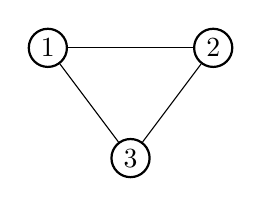
\begin{tikzpicture}
      \begin{scope}[scale=0.7]
        \tikzstyle{cnode} = [thick, draw=black, circle, inner sep = 2pt,  align=center]
        \node[cnode] (x1) at (0,0) {$1$};
        \node[cnode] (x2) at (3,0) {$2$};
        \node[cnode] (x3) at (1.5,-2) {$3$};
        \draw[-] (x1) -- (x2);
        \draw[-] (x1) -- (x3);
        \draw[-] (x2) -- (x3);
      \end{scope}
    \end{tikzpicture}
  \end{subfigure}
  \begin{subfigure}{0.3\textwidth}
    \begin{tabular}{llc}
      \toprule
      $X_1$ & $X_2$ & $\phi(X_1, X_2)$ \\
      \midrule
      0  &  0  &  10 \\
      0  &  1  &  1 \\
      1  &  0  &  1 \\
      1  &  1  &  10\\
      \bottomrule
    \end{tabular}
  \end{subfigure}
  \begin{subfigure}{0.05\textwidth}
    \centering
    \begin{tikzpicture}
      \node[] at (0,0) {$\cdots$};
    \end{tikzpicture}
  \end{subfigure}
  \begin{subfigure}{0.3\textwidth}
    \begin{tabular}{llc}
      \toprule
      $X_2$ & $X_3$ & $\phi(X_1, X_2)$ \\
      \midrule
      0  &  0  &  5 \\
      0  &  1  &  3 \\
      1  &  0  &  3 \\
      1  &  1  &  5 \\
      \bottomrule
    \end{tabular}
  \end{subfigure}
  \caption{A Markov random field with three binary nodes. Potential factors are represented by tables.}
  \label{chp2:fig:toy_mrf}
  \hspace{1cm}
\end{figure}

\begin{example}\label{chpt2:mrf-3node-example}
  As shown in Figure~\ref{chp2:fig:toy_mrf}, the MRF encodes dependency of three random variables $X_1$, $X_2$, and $X_3$, where node $i$ is associated with variable $X_i$ and each has a binary domain, i.e. $\Xx_i = {0,1}$ for $i =1,2,3$. Three potential factors of the MRF together define the joint distribution
  \begin{equation*}
    p(\bm{x}) = \frac{1}{Z} \phi_{1,2}(x_1, x_2) \phi_{2,3}(x_2, x_3) \phi_{1,3}(x_1, x_3)
  \end{equation*}
  where $Z = \sum_{x_1, x_2, x_3}\phi_{1,2}(x_1, x_2) \phi_{2,3}(x_2, x_3) \phi_{1,3}(x_1, x_3)$ normalizes the potential factors such that $p(\bm{x})$ sums to one. The exemplified potential factors in Figure~\ref{chp2:fig:toy_mrf} demonstrate that it is more compatible or likely when $X_1$, $X_2$ and $X_3$ are in the same state (either $0$ or $1$) than they are configured into different states.
\end{example}

From the above example to a formal statement, a MRF over random vector $\bm{X}$ can be represented by a undirected graph $\Gg(\Vv, \Ee)$, with each node $i \in \Vv$ is associated with a random variable $X_i$ and undirected edge set $\Ee \subset \Vv \times \Vv$. This MRF encodes a collection of distributions that factorize as
\begin{equation}\label{chp2:eq:mrf-definition}
  p(\bm{x};\bm{\theta}) = \frac{1}{Z(\bm{\theta})} \prod_{\alpha \in \Ii} \phi_{\alpha}(\bm{x_{\alpha}};\bm{\theta}),
\end{equation}
where $\Ii$ is the set of indexes of potential factors, and each factor $\phi_{\alpha}$ for $\alpha\in \Ii$ is defined on subset of $\bm{X}$, i.e. $\phi_{\alpha}: \Xx_{\alpha} \rightarrow \RR^{+} \cup \{0\}$, where $\Xx_{\alpha} = \prod_{i\in \alpha}\Xx_i$ is the domain of potential factor $\phi_{\alpha}$. The scope of factor $\alpha$ is $\bm{X}_{\alpha} = \left\{ X_i| i\in \alpha \right\}$. In \eqref{chp2:eq:mrf-definition},
\begin{equation}
  Z(\bm{\theta}) = \sum_{\bm{x}} \prod_{\alpha \in \Ii} \phi_{\alpha}(\bm{x_{\alpha}};\bm{\theta})
\end{equation}
is the \textit{partition function}. Apparently, the partition function normalizes the potential factors such that $p(\bm{x}; \bm{\theta})$ is a proper probability.

\begin{remark}
  We can compare directed and undirected graphical models with regarding the following aspects.
  \begin{itemize}
  \item \textit{Representation}: The structure and the parameters directed graphical models provide a natural representation for many types of real-world domains. MRF representation is not usually as intuitive as directed graphical models. But the acyclic property of directed graphical models also limits their representation power. On the other hand, MRFs can be either cyclic or acyclic, which offers the flexibility of graph structure and can simplify the graphical representation. Due to the requirement is weaker for potential factors than that for conditional distribution, the representation of MRFs are richer. 
  \item \textit{Local nonnegative functions}: The local functions are conditional probability functions in directed graphical models, but are potential factors (nonnegative) in undirected cases.
  \item \textit{Sampling}: Sampling is more straightforward within generative models (directed) than that in MRFs.
  \item \textit{Normalization}: Since each local function is a conditional probability function in directed graphical models, partition function for normalization is not needed. A MRF in general comes with partition functions, since the requirement on potential factors are weaker than a conditional probability distribution.
  \end{itemize}
\end{remark}




\subsection{Alternative Representation of MRF}
\begin{figure}[!t]
  % \captionsetup[subfigure]{justification=centering}
  \begin{subfigure}{.5\textwidth}
    \centering
    \begin{tikzpicture}
      \begin{scope}[scale=0.7]
        \tikzstyle{cnode} = [thick, draw=black, circle, inner sep = 2pt,  align=center]
        \tikzstyle{nnode} = [thick, rectangle, rounded corners = 0pt,draw,inner sep = 5pt]
        \node[cnode] (x1) at (0,0) {$1$};
        \node[above=0.2mm of x1] {$X_1$};
        \node[cnode] (x2) at (3,0) {$2$};
        \node[above=0.2mm of x2] {$X_2$};
        \node[cnode] (x3) at (1.5,-2) {$3$};
        \node[below=0.2mm of x3] {$X_3$};

        \node[nnode] (f12) at (1.5, 0) {};
        \node[] at ($(f12) + (0,0.6)$) {$\phi_{1,2}$};
        \node[nnode] (f13) at (0.75, -1) {};
        \node[] at ($(f13) + (-0.8,0)$) {$\phi_{1,3}$};
        \node[nnode] (f23) at (2.25, -1) {};
        \node[] at ($(f23) + (0.80,0)$) {$\phi_{2,3}$};
        \path[-, draw, thick]
        (x1) edge node {} (f12)
        (f12) edge node {} (x2)
        (x2) edge node {} (f23)
        (f23) edge node {} (x3)
        (x3) edge node {} (f13)
        (f13) edge node {} (x1)
        ;
      \end{scope}
      
    \end{tikzpicture}
    \caption{Factor graph representation.}
    \label{chpt2:fig:factor-graph-3node-example}
  \end{subfigure}
  \begin{subfigure}{.5\textwidth}
    \centering
    \begin{tikzpicture}
      \begin{scope}[scale=0.7]
        \tikzstyle{cnode} = [thick, draw=black, circle, inner sep = 2pt,  align=center]
        \tikzstyle{cfnode} = [thick, draw=black, fill=gray,circle, inner sep = 2pt,  align=center]
        \tikzstyle{nnode} = [thick, rectangle, rounded corners = 0pt,draw,inner sep = 5pt]
        \node[cnode] (x1) at (0,0) {$1$};
        \node[above=0.2mm of x1] {$X_1$};
        \node[cfnode] (x2) at (3,0) {$2$};
        \node[above right=0.2mm and 0.2mm of x2] {$X_2=x_2$};
        \node[cnode] (x3) at (1.5,-2) {$3$};
        \node[below=0.2mm of x3] {$X_3$};
        \node[nnode] (f12) at (1.5, 0) {};
        \node[] at ($(f12) + (0.2,0.6)$) {$\phi_{1,2}\bm{1}(x_2)$};
        \node[nnode] (f13) at (0.75, -1) {};
        \node[] at ($(f13) + (-0.8,0)$) {$\phi_{1,3}$};
        \node[nnode] (f23) at (2.25, -1) {};
        \node[] at ($(f23) + (1.50,0)$) {$\phi_{2,3}\bm{1}(x_2)$};
        \path[-, draw, thick]
        (x1) edge node {} (f12)
        (f12) edge node {} (x2)
        (x2) edge node {} (f23)
        (f23) edge node {} (x3)
        (x3) edge node {} (f13)
        (f13) edge node {} (x1)
        ;
      \end{scope}
    \end{tikzpicture}
    \caption{Conditioning on $X_2=x_2$}
    \label{chpt2:fig:factor-graph-3node-example-condition}
  \end{subfigure}

  \caption{A Markov random field is represented by a factor graph, i.e. \ref{chpt2:fig:factor-graph-3node-example}, and conditioning of the Markov random field \ref{chpt2:fig:factor-graph-3node-example-condition}.}
  \label{chp2:tab:toy-factor-graph}
  \hspace{1cm}
\end{figure}

The representation of a MRF by $\Gg(\Vv, \Ee)$ as explained above is compact, but the potential factors are missing. An alternative representation of MRF is \textit{factor graph} \cite{kschischang2001factor_graph},
which is a bipartite graph topology. In a factor graph, a potential factor is explicitly represented as a factor node, as counterpart of variable node associated with a random variable.
\begin{definition}\label{chpt2:def:factor-graph}
  A factor graph $\Gg_F$, is a bipartite graph that represents the factorization structure of \eqref{chp2:eq:mrf-definition}. A factor graph has two types of nodes: i) a variable node for each variable $x_i$; ii) a factor node for each potential function $\phi_{\alpha}$. An edge between a variable node $i$ and factor node $\alpha$ if and only if $x_i$ is argument of $\phi_{\alpha}$. We would denote a factor graph by $\Gg_F(\Vv \cup \Ff, \Ee_F)$ with $\Vv$ as the set of variable nodes, $\Ff$ as the set of factor nodes, and $\Ee_F$ the set of undirected edges.
\end{definition}
\begin{example}
  Let us represent the Example~\ref{chpt2:fig:factor-graph-3node-example} by a factor graph, which is shown in Figure~\ref{chpt2:fig:factor-graph-3node-example}. Different from the representation by $\Gg(\Vv, \Ee)$ in Figure~\ref{chp2:fig:toy_mrf}, factor nodes are explicitly represented by square nodes.
\end{example}


\subsection{Conditioning on Observations in MRFs}
It is not rare that a graphical model may contain observed variable. The node set of a MRF can be separated into a subset $\Vv_O$ of nodes, that are associated with observed variable $\bm{X}_O$, and a subset $\Vv_U$ of nodes associated with unobserved variable $\bm{X}_U$. For an observation $\bm{X}_O=\bm{x}_O$,
\begin{equation}
  p(\bm{x}_U|\bm{x}_O;\bm{\theta}) = \frac{p(\bm{x}; \bm{\theta})}{p(\bm{x}_O;\bm{\theta})} =  \frac{Z(\bm{x}_O,\bm{\theta})}{Z(\bm{\theta})},
\end{equation}
where 
\begin{align}
  \tilde{p}(\bm{x}; \bm{\theta}) &= \prod_{\alpha \in \Ii} \phi_{\alpha}(\bm{x}_{\alpha};\bm{\theta}), \nonumber \\
  Z(\bm{x}_O, \bm{\theta}) &= \sum_{\bm{x}_U} \tilde{p}(\bm{x}; \bm{\theta}), \nonumber \\
  Z(\bm{\theta}) &= \sum_{\bm{x}_O}\sum_{\bm{x}_U} \tilde{p}(\bm{x}; \bm{\theta}).
\end{align}
This means that a condition probability can be computed by partition function and sub-partition functions. Alternatively, the conditional probability can be written as
\begin{equation}
  p(\bm{x}_U|\bm{x}_O;\bm{\theta}) = \frac{\tilde{p}(\bm{x}; \bm{\theta})\bm{1}(\bm{x}_O)}{\sum_{\bm{x}_U}\tilde{p}(\bm{x}; \bm{\theta})\bm{1}(\bm{x}_O)}
\end{equation}

where $\bm{1}(\bm{x}_O)$ is an indicator function and equals to one if and only if the states of nodes in $\Vv_O$ are jointly $\bm{x}_O$. This can be understood as clamping nodes in $\Vv_O$ of the MRF to configuration $\bm{x}_O$, i.e. the domain of $\bm{X}_O$ becomes a set containing only $\bm{x}_O$. (For instance, an example of conditioning on a variable node is shown in Figure~\ref{chpt2:fig:factor-graph-3node-example-condition}.) Then any inference applicable to a MRF applies to the MRF with nodes clamped as well.

In addition to the above intuitions, conditioning can also be understood as a process of reducing the graph of a MRF. When a MRF is conditioned on $\bm{x}_O$, the variables nodes of set $\Vv_O$ are removed from $\Gg$, along with their edges. The potential factors with regarding to $\Vv_U$ are modified accordingly \cite[Chapter~4.2.3]{koller2009pgm}.

It can be seen that MRF framework is capable to handle conditioning as well. Therefore, in the following part of the thesis, it might or might not have bee based on conditioning observed variables when a MRF is mentioned.

\section{Divergence}\label{chpt2:sec:devergence}
Before we get into more discussion about inference and learning topics, we firstly introduce the concept of \textit{divergence} measures since principles of both learning and inference are closed related with divergence measure.
A divergence measure play a fundamental role when we try to use a probability density (or mass for discrete cases) function $q$ to approximate another probability density function $p$. A divergence measure is used to formal quantity how much information is lost when $p$ is represented by $q$. Denote $\PP$ as the space of measures $p$ and $q$, i.e. $p, q \in \PP$.
\begin{definition}
  Given the space of probability density (or mass) function $\PP$ for a random variable $\bm{x}$, a divergence on this space is defined as a function $D(p\|q): \PP \times \PP \rightarrow \RR$ such that $D(p\|q) \geq 0$ for all $p, q \in \PP$ and $D(p\|q)=0$ if and only if $p=q$.
\end{definition}

Here we introduce the classic \textit{Kullback-Leibler divergence} \cite{kullback1959, kullback1951}, KL divergence for short, which is one of the most widely used divergence measures in machine learning, statistics and information theory.
\begin{definition}
  The Kullback-Leibler (KL) divergence on $\PP$ is defined as a function $KL(\cdot \| \cdot): \PP \times \PP \rightarrow \RR^{+} \cup {0}$ with the following form
  \begin{equation}\label{chpt2:def:kl-divergence}
    \mathrm{KL}(p\|q) = \sum_{\bm{x}}p(\bm{x}) \log{\frac{p(\bm{x})}{q(\bm{x})}},
  \end{equation}
  where $\log$ is the natural loggarithm. Note the sum in \ref{chpt2:def:kl-divergence} should be replaced by intergral when $p$ and $q$ are probability density functions.
\end{definition}


KL divergence is not symmetric. In another word, there is no equivalence between $\mathrm{KL}(p\|q)$ and $\mathrm{KL}(q\|p)$ in general. 



\section{Inference Tasks}
\label{sec:background-graphial-reppresentation}

Given a probability distribution $p(\bm{x})$ as the underline distribution of a graphical model, inference in general can be generally divided into four kinds of tasks, as brought up in Chapter~\ref{chpt1:sec:scope-outline}. Our work in this thesis would closed involved with the problems
\begin{itemize}
\item computing the likelihood of observed data or unobserved random variable;
\item computing the marginals distribution over a particular subset of nodes, i.e. $p(x_A)$ for $A \in \Vv$. Note that single-node marginal distribution $p(x_i)$ also belongs to this case;
\item computing the conditional distribution a subset of nodes given the configuration of another subset of nodes, i.e. $p(\bm{x}_A| \bm{x}_B)$ for $A, B \in \Vv$ and $A \cap B = \emptyset$;
\end{itemize}
in MRFs. The above tasks are also close related with the inference of partition function
\begin{itemize}
\item Computation of $Z(\bm{\theta}) = \sum_{\bm{x}} \prod_{\alpha \in \Ii} \phi_{\alpha}(\bm{x_{\alpha}};\bm{\theta})$, or sub-partition functions.
\end{itemize}



\section{Variational inference}
\textcolor{red}{fix notation and consistency in this section}

In solving inference tasks, one important technique is based on a variational approach. With $p(\bm{x})$ as the underlining probability distribution of a graphical model, directly inference with $p(\bm{x})$ is often unfeasible due to the system represented by the graphical model is too large or complex (Even we know the form of $p(\bm{x})$, the computation in inference tasks can be prohibitive). In variational approach, a 'trial' probability distribution $b(\bm{x})$ is introduced to approximate $p(\bm{x})$. The trial distribution should be intuitively simpler than $p(\bm{x})$. 
\textit{Variational free energy} \cite{opper2001advanced} is used to find such a approximation, which uses a probability distribution $b(\bm{x})$ to approximate $p(\bm{x};\bm{\theta})$. The variational free energy is defined by
\begin{align}
  F_V(b) & = KL(b( \bm{x}) || p(\bm{x}; \bm{\theta})) - \log{Z(\bm{\theta})} \nonumber \\
         &= \sum_{\bm{x}}b(\bm{x}) \ln{\frac{b(\bm{x})}{{p}(\bm{x}; \bm{\theta})}} - \ln{Z(\bm{\theta})} \nonumber \\
         & = \sum_{\bm{x}}b(\bm{x}) \ln{\frac{b(\bm{x})}{\tilde{p}(\bm{x}; \bm{\theta})}} 
\end{align}

where $\tilde{p}(\bm{x}; \bm{\theta}) =  \prod_{\alpha \in \Ii} \psi_{\alpha}(\bm{x}_{\alpha}; \bm{\theta}_{\alpha})$. Since $\mathrm{KL}(b(\bm{x})\|p(\bm{x};\bm{\theta}))$ is always non-negative and is zero if and only if $b(\bm{x}) = p(\bm{x};\bm{\theta})$, we have $F_V(b) \geq - \log{Z(\bm{\theta})}$, with equality when $b(\bm{x}) = p(\bm{x};\bm{\theta})$.

\subsection{Variational Free Energy and Mean Field}

In mean field approach, a fully-factorized approximation is used,
\begin{equation}\label{eq:mf-factorization}
  b_{MF}(\bm{x}) = \prod_{i=1}^{n}b_i(x_i).
\end{equation}
Substituting \eqref{eq:mf-factorization} into the variational free energy gives
\begin{align}
  F_{MF} = & - \sum_{a}\sum_{\bm{x}_{\alpha}} \ln{\psi_{\alpha}(\bm{x}_{a};\bm{\theta})}
             \prod_{i\in \mathrm{ne}_{\alpha}}b_i(x_i) \nonumber\\
           &+ \sum_i \sum_{x_i} b_i(x_i) \ln{b_i(x_i)},
\end{align}
where $\mathrm{ne}_{\alpha} = \left\{ i \in \Vv | x_i \in \Ss(a) \right\}$ gives the neighboring variable nodes of factor $a$, and $\Ss(a)$ is the scope set (arguments) of factor node $a$.
Solving the minimization of $F_{MF}$ w.r.t. $b_{MF}(\bm{x})$ gives the
update rule of mean field
\begin{equation}
  \ln{b_i(x_i)} \sim \sum_{a\in \mathrm{ne}_i} \sum_{\bm{x}_{\alpha} \backslash x_i} \ln{\psi_{\alpha}}(\bm{x}_{\alpha};\bm{\theta}_{\alpha}) \prod_{j\in \mathrm{ne}_{\alpha}\backslash i} b_j(x_j),
\end{equation}
where $\mathrm{ne}_i = \left\{ a | i \in \Ss(a), a \in \Ff \right\}$, i.e. the
neighboring factors of node $i$.

\subsection{Bethe Free Energy and (Loopy) Belief Propagation}


Different from the mean field approximation, Bethe approximation also includes the non-single-node beliefs $\{b_{\alpha}(\bm{x}_{\alpha})\}$ apart from the single-node beliefs $\{b_i(x_i)\}$\cite{yedidia2003understanding}. In this case, the Bethe free energy is given by
\begin{align}\label{apdix:bethe-free-energy}
  F_{Bethe} = &\sum_{a} \sum_{\bm{x}_{\alpha}}
                b_{\alpha}(\bm{x}_{\alpha})\ln{\frac{b_{\alpha}(\bm{x}_{\alpha})}{\psi_{\alpha}(\bm{x}_{\alpha})}
                } \nonumber \\
              & -  \sum_{i=1}^{N} (|\mathrm{ne}_i| - 1) \sum_{x_i} b_i(x_i) \ln{b_i(x_i)}.
\end{align}
Due to the  non-single-node beliefs, there are consistency constrains $\sum_{\bm{x}_{\alpha}} b_{\alpha}(\bm{x}_{\alpha}) = \sum_{ x_i} b_i({x}_i) =1$, $\forall~ i \in \Ss(a)$ to obey. Then, solving the Bethe free energy minimization problem
\begin{align}
  \min_{\{b_{\alpha}(\bm{x}_{\alpha})\}, \{b_i(x_i)\}}& F_{Bethe} \nonumber \\
  \mathrm{s.t.}~~ & \sum_{\bm{x}_{\alpha} \backslash x_i} b_{\alpha}(\bm{x}_{\alpha})  =
                    b_i(x_i), \nonumber \\
                                                      & \sum_{\bm{x}_{\alpha}} b_{\alpha}(\bm{x}_{\alpha}) = \sum_{ x_i} b_i({x}_i) =1,
                                                        \nonumber \\
                                                      &  0 \leq b_i(x_i) \leq 1,  \nonumber \\
                                                      &  b_{\alpha}(\bm{x}_{\alpha}) \in [0,1]^{|S(\bm{x}_{\alpha})|\times K}, \nonumber \\
                                                      & i \in \Vv , a \in \Ff,
\end{align}
where $\Vv$ and $\Ff$ are the set of variable nodes and the set of
factor nodes in factor graph as defined in
Definition~\ref{chpt2:def:factor-graph}, gives the (loopy) BP message-passing rule
\begin{equation}
  m_{a\rightarrow i}(x_i) \sim \sum_{\bm{x}_{\alpha} \backslash x_i}
  \psi_{\alpha}(\bm{x}_{\alpha}) \prod_{j \in \Ss(a) \backslash i} \prod_{b \in \mathrm{ne}_j
    \backslash a} m_{b\rightarrow j}(x_j).
\end{equation}


\section{Learning principles}
We have touched the learning topic in \autoref{chapter1}, which is to find the 'best' probability distribution $p(\bm{x}; \bm{\theta})$ in its space $\PP$. To make the discussion more concrete, we assume the domain is governed by a underlying distribution $p^{\ast}$ that is induced by a (directed or undirected) graphical model, $\Mm = \left\{ \Kk^{\ast}, \bm{\theta}^{\ast} \right\}$ with $\Mm^{\ast}$ representing its structure and $\bm{\theta}^{\ast}$ representing its parameter. Here we discuss about \textit{model learning} (parameter learning only). For notation simplicity, we use $p^{\ast}(\bm{x})$ to denote this distribution. We are given a dataset $\Dd = \{\bm{x}^{1}, \bm{x}^{2}, \cdots, \bm{x}^{M}\}$. Following the standard assumption, these sample instances are \textit{independent and identically distributed (i.i.d.)}. The task is then to use the information from the dataset to learn a distribution $p$ within its space $\PP$, since the governing distribution $p^{\ast}(\bm{x})$ is not known.

The problem of learning a distribution in $\PP$ to approximate $p^{\ast}$ can be formulated as density estimation. With the concept of KL divergence in \autoref{chpt2:sec:devergence}, learning of $p$ can be formulated as minimizing the KL divergence
\begin{align}\label{chpt2:sec:mle-as-min-kl}
  &\mathrm{KL}(p^{\ast}(\bm{x})\|p(\bm{x}; \bm{\theta})) \nonumber \\
  =& \EE_{\bm{x} \sim p^{\ast}}\left[ \log{\frac{p^{\ast}(\bm{x})}{p(\bm{x}; \bm{\theta})}} \right] \nonumber \\
  =& - H(p^{\ast}) - \EE_{\bm{x} \sim p^{\ast}}\left[ \log{{p(\bm{x}; \bm{\theta})}} \right],
\end{align}
where $H(p^{\ast})$ is the entropy of $p^{\ast}$.
Due to the property of divergence, the KL divergence in \ref{chpt2:sec:mle-as-min-kl} is zero if and only if $p(\bm{x};\bm{\theta})=p^{\ast}(\bm{x})$. The last line of \ref{chpt2:sec:mle-as-min-kl} shows that the negative entropy term does not depends on $p(\bm{x}; \bm{\theta})$. Thus we can just focus on the expectation term $\EE_{\bm{x} \sim p^{\ast}}\left[ \log{{p(\bm{x}; \bm{\theta})}} \right]$, which is \textit{expected log-likelihood}. Therefore, we can just use the expected log-likelihood to do model learning instead of minimizing the KL divergence.

Note although we can use the expected log-likelihood for model learning task and even model comparison (comparing a trained model with another one), we loss the information of how close a trained model is to $p^{\ast}$. This is due to the omitting of $H(p^{\ast})$, which is not available.

Since it is not possible to know $p^{\ast}$ (otherwise we do not need to learn it), the expected log-likelihood is approximated by sample instances of $p^{\ast}$,
\begin{equation}
  \Ll(\Dd; \bm{\theta}) = \frac{1}{\abs{\Dd}}\sum_{\bm{x}\in \Dd}\log{p(\bm{x};\bm{\theta})},
\end{equation}
and
\begin{equation}
  \EE_{\bm{x}\sim p^{\ast}}(\log{{p(\bm{x}; \bm{\theta})}}) \approx \Ll(\Dd; \bm{\theta}).
\end{equation}

Log-likelihood $\Ll(\Dd; \bm{\theta})$ is one of the most widely used loss for model learning. However, $\Ll(\Dd; \bm{\theta})$ is not always a feasible loss to compute due to:
\begin{itemize}
\item exact computation of $p(\bm{x})$ is not possible;
\item there are some elements of $\bm{x}$ which are not observable (hidden variables).
\end{itemize}
For the first case, the typical treatment is to approximate the exact log-likelihood. This is done by approximation with employing inference methods or   making simplified assumptions on dependency structure of the graphical model of $p(\bm{x})$. Then, optimization is carried out with regarding to the approximated log-likelihood. These methods include surrogate likelihood \cite{wainwright06estimating, lu2019blockBP}, pseudo-likelihood\cite{qu2019gmnn}, piecewise likelihood \cite{sutton2012piecewise, lin_2016_CVPR}, saddle-point approximation \cite{srikumar-etal-2012-amortizing, NIPS2019_9687}.

For the second case that there are hidden variables,
1. EM

2. variational EM

3. a bit Bayesian ?

1. begin with KL minimization, refer to \cite[chapter16]{koller2009pgm}



2. talk a bit of others learning objectives, refer to Domke 2013 paper.
\subsection{Learning of Full Observation}

the learning diagram here
\begin{itemize}
\item Structural learning
\item parameter learning
\end{itemize}


the learning principle:
\begin{itemize}
\item Maximal likelihood estimation (MLE)
\item Bayesian estimation
\item Maximal conditional likelihood
\item Maximal '' `Margin`''
\item Maximum entropy
\end{itemize}


It may be better to discuss the learning principle here.

Cited from 10-708 lecture6 note:

UNOBSERVED VARIABLES:

A variable can be unobserved or latent because it is a(n):

-Abstract or imaginary quantity meant to simplifiy the data generation process, e.g. speech recognition models, mixture models.
-A real-world object that is difficult or impossible to measure, e.g. the temperature of a star, causes of disease, evolutionary ancestors.
-A real-world object that was not measured due to missed samples, e.g. faulty sensors.

Discrete latent variables can used to partition or cluster data into sub-groups

Continuous latent variables (factors) can be used for dimensionality reduction (e.g. factor analysis, etc)
\subsection{Dealing with latent variables}
\subsection{about clamping node}
clamping node gives conditional distribution.

\subsection{about ELBO bound}
1. the bound used by EM

2. talk about ELBO/variational inference \href{https://media.nips.cc/Conferences/2016/Slides/6199-Slides.pdf}{Variational Inference}, which is closely related the bound used in EM.

%%% Local Variables:
%%% mode: latex
%%% TeX-master: "../../main"
%%% End:


\part{Inference}
\label{part:inference}
% chapter 3
\chapter{An Alternative View of Belief Propagation}
\label{chapter3}
% set the path to figures in this section
\graphicspath{{source/chapter3/}}

Belief propagation (BP) is a meta message-passing algorithm for inference problems in probabilistic graphical models. BP answers queries by locally exchanging beliefs (statistical information) between nodes in a graphical model \cite{kschischang2001factor_graph, Bishop:2006:PRM:1162264}. In Section~\ref{chpt2:sec:variational-inference}, we introduced the classic belief propagation as the minimization of free energy, instead of an iterative message-passing routine. Interesting to note, the message-passing rule of BP was developed as early as $1986$ \cite{pearl1986b} and had been popularly used in different fields before the free energy optimization intuition was developed in literature \cite{yedidia2003understanding}.

BP can solve inference problems in linear-time exactly when graphs are loop-free or tree-structured \cite{kschischang2001factor_graph}. The message-passing routine of BP can be boiled down into variable elimination in tree-structured graphs\footnote{This applies to cases where systems themselves can be represented by tree-structured graphs, or cases where original graphs are not trees but becoming tree-structured after reorganized (such as clustering).} and message scheduling, which corresponds to determining the variable elimination order. The message scheduling can be omitted and equivalent exact inference results can be obtained, when an alternative belief update algorithm is applied which is also known as Lauritzen-Spiegelhalter algorithm \cite[Section~10.3]{koller2009pgm}. BP and its variants are widely applied in large computation systems due to their 'magic' of reducing the exponential number of operations for inference with enumeration into linear complexity. This is possible because: 
\begin{itemize}
\item An underline distribution of a graphical model is usually factorized, and each sub-expression (a factor) depends only on a small number of variables.
\item The intermediate results are computed once and cached as messages, which are reused in coming computations. 
\end{itemize}

Inevitably, many real-world signals are naturally modeled by graph representations with loops. Surprisingly, although lost its optimality guarantees in loopy graphs, loopy BP is still a practical method and gives reasonable good inference results by running it as if there ware no loops. But its performance can vary from case to case and its behavior is not well understood in general. 

In this chapter, to gain more insights into BP in general graphs, we take a variational approach to develop an interpretable variant of BP, which is termed as $\alpha$-BP.
The intuition of $\alpha$-BP starts with a surrogate distribution $q(\bm{x})$, which is an approximate distribution. $q(\bm{x})$ is assumed to be fully factorized, and each factor of $q(\bm{x})$ actually represents a message in the graphical model with an underlining distribution $p(\bm{x})$. We derive a message-passing rule that is induced by minimizing a localized $\alpha$-divergence. The merits of $\alpha$-BP are as follows: i). {$\alpha$-BP is derived intuitively as localized minimization of $\alpha$-divergence between original distribution $p$ and surrogate distribution $q$}; ii). {$\alpha$-BP generalizes the standard BP, since the message-passing rule of BP is a special case of $\alpha$-BP}. iii). {$\alpha$}-BP can outperform BP in complete (fully-connected) graphs while still maintaining the simplicity of BP for inference.

Apart from the algorithmic perspective, another common issue of BP and its variants in general graphs is convergence. We devote Section~\ref{chpt3:sec:cnvg-thm} to a convergence study of $\alpha$-BP. Sufficient conditions that guarantee the convergence of $\alpha$-BP to a unique fixed point, are studied and obtained. It turns out that the derived convergence conditions of $\alpha$-BP depend on both the graph and also the value of $\alpha$. This result suggests that a proper choice of $\alpha$ can help to guarantee the convergence of $\alpha$-BP.

\section{$\alpha$ Divergence}
\label{chpt3:sec:alpha-divergence}
Before we get into the algorithmic discussion, we firstly provide some preliminaries for the algorithmic intuition. As an extended discussion to Section~\ref{chpt2:sec:devergence}, we firstly introduce a more generalized divergence than $\mathrm{KL}$ divergence.

Apart from the KL divergence, another divergence measure that generalizes KL divergence is $\alpha$-divergence. In fact, $\alpha$-divergence appeared in literature just one year later than KL divergence when Herman Chernoff initially defined it for likelihood-ratio tests \cite{Chernoff1952measure}. Around a decade later, Alfr\'ed R\'enyi proposed his version of divergence as well \cite{renyi1961entropy}. In the 80s of last century, Amari extended Chernoff's version of $\alpha$-divergence \cite{amari1982differential}, which is now widely used in studies of the geometry of distribution manifolds. 
$\alpha$-divergence, similar to KL divergence, is a typical way to measure how different two measures characterized by densities $p$ and $q$ are. By following the notation \cite{Zhu95informationgeometric}, the definition of $\alpha$-divergence (Amari's version, with correction term to accommodate unnormalized measure) is as follows,
\begin{equation}\label{chpt3:eq:alpha-divergence}
  \Dd_{\alpha}(p \| q ) = \frac{\sum_{\bm{x}} \alpha p(\bm{x}) + (1-\alpha) q (\bm{x}) - p(\bm{x})^{\alpha} q(\bm{x})^{1-\alpha}}{\alpha(1-\alpha)},
\end{equation}
where $\alpha$ is the parameter of this divergence. Different from the KL divergence definition in Section~\ref{chpt2:sec:devergence}, $p$ and $q$ here are not necessarily to be normalized measures.

In Section~\ref{chpt2:sec:devergence}, the KL divergence was defined over two normalized measures. Here we extend that definition to a generalized case where $p$ and $q$ are not necessarily normalized, as an extended divergence from the normalized case. As shall be see, KL divergence is closely related with $\alpha$-divergence. KL divergence for general measures is defined as
\begin{equation}\label{chpt3:eq:kl-divergence}
  \mathrm{KL}(p \| q) = \sum_{\bm{x}} p(\bm{x}) \log{\frac{p(\bm{x})}{q(\bm{x})}} + \sum_{\bm{x}} q(\bm{x}) - p(\bm{x}) ,
\end{equation}
where the $\sum_{\bm{x}} q(\bm{x}) - p(\bm{x})$ is a correction factor to accommodate possibly unnormalized $p$ and $q$.
\begin{remark}
  The KL divergence can be seen as a special case of $\alpha$-divergence, by observing $\lim_{\alpha \rightarrow 1}\Dd_{\alpha}(p \| q ) = KL(p\|q)$ and $\lim_{\alpha \rightarrow 0}\Dd_{\alpha}(p \| q ) = KL(q\|p)$ (applying L'H\^opital's rule to \eqref{chpt3:eq:alpha-divergence}).

  Regarding the basic properties of divergence measures, both $\alpha$-divergence and KL divergence are zero when $p=q$, and they are non-negative. 
\end{remark}

Denote the KL-projection by
\begin{equation}
  \text{proj}[p] = \uargmin{q \in \Qq} \mathrm{KL}(p\|q),
\end{equation}
where $\Qq$ is a family of distributions that $q$ belongs to.
According to the stationary point equivalence Theorem in \cite{divergence-measures-and-message-passing}, $\text{proj}[p^{\alpha}q^{1- \alpha}]$ and $\Dd_{\alpha}(p\|q)$ have same stationary points (gradient is zero). This equivalence holds by assuming $\theta$ is parameter of $q(x)$ and observing
\begin{align}
  \pd{\mathrm{KL}(p\|q)}{\theta} &= \sum_{\bm{x}} \pd{q(\bm{x})}{\theta} - \sum_{\bm{x}}\frac{p(\bm{x})}{q(\bm{x})} \pd{q(\bm{x})}{\theta} , \nonumber \\
  \pd{\mathrm{\Dd_{\alpha}}(p\|q)}{\theta} &= \frac{1}{\alpha} \left( \sum_{\bm{x}} \pd{q(\bm{x})}{\theta} - \sum_{\bm{x}}\frac{p^{\prime}(\bm{x})}{q(\bm{x})} \pd{q(\bm{x})}{\theta} \right), \nonumber
\end{align}
with $p^{\prime}(\bm{x}) = p^{\alpha}(\bm{x})q(\bm{x})^{1-\alpha}$. Then it gives $\pd{\mathrm{\Dd_{\alpha}}(p\|q)}{\theta}  = \frac{1}{\alpha}\pd{\mathrm{KL}(p\|q)}{\theta}|_{p=p^{\prime}}$.

A heuristic scheme to find $q^{\ast}$ minimizing $\Dd_{\alpha}(p\|q)$ starts with an initial $q$, and repeatedly updates $q$ via the projection on $\Qq$
\begin{equation}\label{eq:fixed-point-iter}
  q(\bm{x})^{\text{new}}  = \text{proj}[p(\bm{x})^{\alpha}q(\bm{x})^{1-\alpha}].
\end{equation}
This heuristic scheme is a fixed-point iteration, which does not guarantee to converge.

\begin{remark}
  We take $\bm{x}$ to be discrete by default in this section. The sum operation should be replaced by integral for continuous variable $\bm{x}$.
\end{remark}

\section{$\alpha$ Belief Propagation Algorithm}\label{sec:alpha-bp-factor-refine}

\subsection{Pairwise MRF}

\begin{figure}
  \begin{centering}
    \begin{tikzpicture}
      % \tikzstyle{enode} = [thick, draw=blue, circle, inner sep = 3pt,
      % align=center]
      \tikzstyle{enode} = [thick, draw=black, circle, inner sep = 4pt, minimum size = 0.7cm, align=center]
      \tikzstyle{nnode} = [thick, rectangle, rounded corners = 0pt, minimum size = 0.5cm,draw,inner sep = 2pt]

      \tikzstyle{cnode} = [thick, cloud, draw,cloud puffs=10, cloud puff arc=120, aspect=2, inner ysep=4pt]

      \node[cnode] (pajk) at (3, 1.5) {$\Nn(t)\backslash s$};
      \node[cnode] (paik) at (-3, 1.5) {$\Nn(s)\backslash t$};

      \node[nnode] (tk) at (0, 1.5) {};
      \node[] at ($(tk) + (0, 0.5)$) {$\phi_{st}(x_s, x_t)$};
      \node[enode] (xi) at (-1.5 ,0) {};
      \node[] at ($(xi) + (0.75,0)$) {$x_s$};
      
      \node[nnode] (fi) at (-1.5 , -1.5) {};
      \node[] at ($(fi) + (0.95,0)$) {$\phi_s(x_s)$};
      

      \node[enode] (xj) at (1.5 ,0) {};
      \node[] at ($(xj) + (0.75,0)$) {$x_t$};
      
      \node[nnode] (fj) at (1.5 , -1.5) {};
      \node[] at ($(fj) + (0.95,0)$) {$\phi_t(x_t)$};
      
      % connections

      \draw[-] (xi) to (fi);
      \draw[-] (xi) to (tk);
      \draw[-] (xi) to (paik);

      \draw[-] (xj) to (fj);
      \draw[-] (xj) to (tk);
      \draw[-] (xj) to (pajk);
    \end{tikzpicture}
    \vskip -0.1in
    \caption{Factor graph illustration of $p(\bm{x})$ in \eqref{eq:mrf}.}\label{fig:factor-graph}
  \end{centering}
\end{figure}


We consider a probability distribution over random vector $\bm{x} = \left(  x_1, x_2, \cdots,  x_N  \right)$, where $\bm{x} \in \bm{\Xx}$ and $\bm{\Xx}=\prod_{i=1}^N\Xx_i$. For explanation simplicity, we define that each domain is instantiated as the same discrete finite set $\Xx$, i.e., $\bm{\Xx}=\prod_{i=1}^N\Xx$ and $x_i \in \Xx$. Note $\alpha$-BP is applicable for the different domain setting $\bm{\Xx}=\prod_{i=1}^N\Xx_i$. Let us denote the undirected graph of a pairwise MRF by $\Gg:=(\Vv, \Ee)$. $\Vv=\left[ 1 : N \right]$ is the node set associated with the index set of entries of $\bm{x}$. The graph contains undirected edges $\Ee \subset \Vv \times \Vv$, where a pair of $(s, t) \in \Ee$ if and only if nodes $s$ and $t$ are connected by an edge. In addition to the undirected edge set, let us also define the directed edge set induced from $\Gg$ by $\vec{\Ee}$. We have $\abs{\vec{\Ee}} = 2\abs{\Ee}$, where $\abs{\cdot}$ denotes the carnality. These directed edges serve the purpose of convergence analysis only.



The joint distribution of $\bm{x}$ can be formulated as a pairwise factorization form in a pairwise MRF as
\begin{equation}\label{eq:mrf}
  p(\bm{x}) \propto \prod_{{s\in \Vv}} \phi_s(x_s) \prod_{(s,t) \in \Ee} \phi_{st}(x_s, x_t),
\end{equation}
where $\phi_{s}: \Xx \rightarrow (0, \infty)$ and $\phi_{st}: \Xx \times \Xx \rightarrow (0, \infty)$ are factor potentials. Here the normalization is omitted. Note the union of the node set and the edge set, i.e. $\Vv \cup \Ee$, instantiates the factor index set $\Ff$ of a general MRF in \eqref{chp2:eq:mrf-definition} here.

The factor graph representation of \eqref{eq:mrf} is shown in
Figure~\ref{fig:factor-graph}. In the figure, $\Nn(s)$ is the set of variable nodes neighboring $x_s$ via
pairwise factors, i.e. $\Nn(s) = \left\{ t|(t,s) \in \Ee \right\}$, and $\backslash$ denotes exclusion.

\subsection{From $\alpha$-divergence minimization to $\alpha$-BP}
We start with defining a surrogate distribution and then use the surrogate distribution to approximate a given distribution. The message passing rule of $\alpha$-BP is derived by solving the distribution approximation problem.

% \subsubsection{Fully Factorized Surrogate}
We begin with defining a distribution
\begin{equation}
  q(\bm{x}) \propto \prod_{{s\in \Vv}} \tilde{\phi}_s(x_s) \prod_{(s,t) \in \Ee} \tilde{\phi}_{st}(x_s, x_t),
\end{equation}
that is similarly factorized as the joint distribution $p(\bm{x})$. The distribution $q(\bm{x})$ acts as a surrogate distribution of $p(\bm{x})$. The surrogate distribution would be used to estimate inference problems of $p(\bm{x})$. We further choose $q(\bm{x})$ such that it can be fully factorized, which means that $\tilde{\phi}_{s,t}(x_s, x_t)$ can be factorized into product of two independent functions of $x_s, x_t$ respectively. We denote this factorization as
\begin{equation}
  \tilde{\phi}_{s,t}(x_s, x_t) := m_{st}(x_t) m_{ts}(x_s).
\end{equation}
We use the notation $m_{ts}(x_s)$ to denote the factor as a function of $x_s$. $m_{ts}: \Xx \rightarrow (0, \infty)$, serves as the message along directed edge $(t \rightarrow s)$ in our algorithm. Similarly we have factor or message $m_{st}(x_t)$. Then the marginal can be formulated straightforwardly as
\begin{equation}
  q_s(x_s) \propto \tilde{\phi}_s(x_s) \prod_{w\in \Nn(s)} m_{ws}(x_s).
\end{equation}

Now, we are going to use the heuristic scheme as in \eqref{eq:fixed-point-iter} to minimize the information loss by using a fully factorized $q(\bm{x})$ to represent $p(\bm{x})$. The information loss is measured by $\alpha$-divergence $\Dd_{\alpha}(p(\bm{x}) \| q(\bm{x}))$.


We perform a factor-wise refinement procedure to update the factors of $q(\bm{x})$ such that $q(\bm{x})$ approximates $p(\bm{x})$. This approach is similar to the factor-wise refinement procedure in assumed density filtering algorithm\cite{ghosh2016assumed, opper1999bayesian} and expectation propagation \cite{divergence-measures-and-message-passing,Minka:2001:EPA:647235.720257}. Without loss of generality, we begin to refine the factor $\tilde{\phi}_{ts}(x_t, x_s)$ via $\alpha$-divergence with its $\alpha$-parameter assignment as $\alpha_{ts}$. Define $q^{\backslash (t,s)}(\bm{x})$ as the product of all other factors excluding $\tilde{\phi}_{ts}(x_t, x_s)$
\begin{align}
  q^{\backslash (t,s)}(\bm{x})
  = q(\bm{x})/\tilde{\phi}_{ts}(x_t,
  x_s) \propto \prod_{{s\in \Vv}} \tilde{\phi}_s(x_s) \prod_{(v,u) \in
  \Ee\backslash (t,s)}
  \tilde{\phi}_{vu}(x_v, x_u).
  % &= \left(
  %   \tilde{\phi}_s(x_s) \prod_{w\in \Nn(s) \backslash t}m_{ws}(x_s)
  % \right)
  % \left(
  %   \tilde{\phi}_t(x_t) \prod_{w\in \Nn(t) \backslash s}m_{wt}(x_t)
  % \right)
  % \left(
  %   \prod_{v \in \Vv \backslash s,t}
  %   \tilde{\phi}_v(x_v) \prod_{w\in \Nn(v)}m_{wv}(x_v)
  % \right)\nonumber \\
\end{align}
We also exclude the factor $\phi_{ts}(x_t, x_s)$ in $p(\bm{x})$ to obtain $p^{\backslash (t,s)}(\bm{x})$. % Assume that we already have had $q^{\backslash (t,s)}(\bm{x})$ as a good approximation of $p^{\backslash (t,s)}(\bm{x})$, i.e. $q^{\backslash (t,s)}(\bm{x}) \approx p^{\backslash (t,s)}(\bm{x})$, where $\approx$ denotes approximately equality, it is $\tilde{\phi}_{ts}(x_t, x_s)$ that remains to be refined. In refining factor $\tilde{\phi}_{ts}(x_t, x_s)$ with $\alpha$-divergence under such assumption, the problem
Instead of updating $\tilde{\phi}_{ts}(x_t, x_s)$ directly by solving
\begin{equation}
  \!\!\!\uargmin{\tilde{\phi}_{ts}^{\mathrm{new}}(x_t, x_s)}\!\!\!\! \Dd_{\alpha_{ts}}\!\!\left(  p^{\backslash (t,s)}\!(\bm{x})\phi_{ts}(x_t, x_s)\|q^{\backslash (t,s)}\!(\bm{x})\tilde{\phi}_{ts}^{\mathrm{new}}(x_t, x_s)\right),
\end{equation}
we consider the following tractable problem
\begin{equation}\label{eq:alpha-minimize-factor}
  \!\!\!\uargmin{\tilde{\phi}_{ts}^{\mathrm{new}}(x_t, x_s)}\!\!\!\!
  \Dd_{\alpha_{ts}}\!\!\left( q^{\backslash (t,s)}\!(\bm{x}){\phi}_{ts}(x_t, x_s)
    \|q^{\backslash (t,s)}\!(\bm{x})\tilde{\phi}_{ts}^{\mathrm{new}}(x_t, x_s) \right),
\end{equation}
which searches for new factor $\tilde{\phi}_{ts}^{\mathrm{new}}(x_t, x_s)$ such $q$ can approximate $p$ better. In \eqref{eq:alpha-minimize-factor}, $\Dd_{\alpha_{ts}}(\cdot)$ denotes the $\alpha$-divergence with the parameter $\alpha_{ts}$. Note that the approximation \eqref{eq:alpha-minimize-factor} is accurate when $q^{\backslash (t,s)}(\bm{x})$ is equal to $p^{\backslash (t,s)}(\bm{x})$. 
Using fixed-point update in \eqref{eq:fixed-point-iter}, the problem in \eqref{eq:alpha-minimize-factor} is equivalent to
\begin{align}\label{eq:update-rule}
  q^{\backslash (t,s)}(\bm{x})\tilde{\phi}_{ts}^{\mathrm{new}}(x_t, x_s) \propto
  % &\propto \text{proj}\left[ \left( q^{\backslash (t,s)}(\bm{x}){\phi}_{ts}(x_t, x_s) \right)^{\alpha_{ts}} \left(q^{\backslash (t,s)}(\bm{x})\tilde{\phi}_{ts}(x_t, x_s)  \right)^{1-\alpha_{ts}} \right] \nonumber \\
  \mathrm{proj}\left[ q^{\backslash
  (t,s)}(\bm{x}){\phi}_{ts}(x_t, x_s)^{\alpha_{ts}} \tilde{\phi}_{ts}(x_t, x_s)^{1-\alpha_{ts}} \right]. 
\end{align}

Without loss of generality, we update $m_{ts}$ and define
\begin{equation}\label{eq:new_ts}
  \tilde{\phi}_{ts}^{\mathrm{new}}(x_t, x_s) = m_{ts}^{\mathrm{new}}(x_s) m_{st}(x_t).
\end{equation}
Since KL-projection onto a fully factorized distribution reduces to matching the marginals \cite[Proposition~8.3]{koller2009pgm}, substituting \eqref{eq:new_ts} into \eqref{eq:update-rule}, we obtain
\begin{align}\label{eq:message-update}
  \sum_{\bm{x}\backslash x_s} q^{\backslash (t,s)}(\bm{x}) \tilde{\phi}_{ts}^{\mathrm{new}}(x_t, x_s) 
  \propto \sum_{\bm{x}\backslash x_s} q^{\backslash (t,s)}(\bm{x}) \phi_{ts}(x_t, x_s)^{\alpha_{ts}} \tilde{\phi}_{ts}(x_t, x_s)^{1-\alpha_{ts}}.
\end{align}
Solving \eqref{eq:message-update} gives the message passing rule as
\begin{align}\label{eq:message-rule-pairwise}
  {m}^{\text{new}}_{ts}(x_s) \propto  m_{ts}(x_s)^{1-\alpha_{ts}} \bigg[\sum_{x_t} \phi_{ts}(x_t, x_s)^{\alpha_{ts}} {m}_{st}(x_t)^{1-\alpha_{ts}}\tilde{\phi}_t(x_t) \prod_{w\in \Nn(t)\backslash s}m_{wt}(x_t) \bigg].
\end{align}

As for the singleton factor $\tilde{\phi}_t(x_t)$, we can do the refinement procedure on $\tilde{\phi}_t(x_t)$ in the same way as we have done on $\tilde{\phi}_{ts}(x_t, x_s)$. This gives us the update rule of $\tilde{\phi}_t(x_t)$ as
\begin{equation}\label{eq:fix-factor-update}
  \tilde{\phi}_t^{\mathrm{new}}(x_t) \propto \phi_t(x_t)^{\alpha_{t}} \tilde{\phi}_t(x_t)^{1-\alpha_{t}},
\end{equation}
which is the belief from factor $\phi_t(x_t)$ to variable $x_t$. Here $\alpha_t$ is the local assignment of parameter $\alpha$ in $\alpha$-divergence in the refining factor $\tilde{\phi}_t(x_t)$. Note, if we initialize $\tilde{\phi}_t(x_t) = \phi_t(x_t)$, then it remains the same in all iterations, which makes
\begin{align}\label{eq:message-rule}
  {m}^{\mathrm{new}}_{ts}(x_s) \propto
  m_{ts}(x_s)^{1-\alpha_{ts}} \bigg[\sum_{x_t} \phi_{ts}(x_t, x_s)^{\alpha_{ts}} {m}_{st}(x_t)^{1-\alpha_{ts}} {\phi}_t(x_t) \prod_{w\in \Nn(t)\backslash s}m_{wt}(x_t) \bigg].
\end{align}
In our notations, a factor potential is undirected, i.e. $\phi_{ts}(x_t, x_s)=\phi_{st}(x_s, x_t)$ for all $(t,s) \in \Ee$. When refining factors with $\alpha$-BP, each factor potential (corresponding to an edge of $\Gg$) can be associated with a difference setting of $\alpha$ value. In addition we also have $\alpha_{ts} = \alpha_{st}$.

\section{Remarks on $\alpha$ Belief Propagation}\label{subsec:remark}

As discussed in Section~\ref{chpt3:sec:alpha-divergence}, $\mathrm{KL}(p\|q)$ is the special case of $\Dd_{\alpha}(p\|q)$ when $\alpha \rightarrow 1$. When restricting $\alpha_{st}=1$ for all $(s,t) \in \Ee$, the message-passing rule in \eqref{eq:message-rule} becomes
\begin{equation}\label{chpt3:eq:bp-update-rule}
  {m}^{\text{new}}_{ts}(x_s) \propto 
  \sum_{x_t} \phi_{st}(x_s, x_t) {\phi}_t(x_t) \prod_{w\in \Nn(t)\backslash s}m_{wt}(x_t),
\end{equation}
which is exactly the messages of standard BP \cite{Bishop:2006:PRM:1162264}. From this point of view, we can say $\alpha$-BP is a generalization of BP. Additionally, the BP update rule in \eqref{chpt3:eq:bp-update-rule} actually corresponds to the fixed-point iteration assignment by solving the Bethe free energy minimization problem in \eqref{chpt2:bethe-free-energy}.


Note although the mean field method also uses fully-factorized approximation, it is obtained differently from $\alpha$-BP and its factorization differs from that of $\alpha$-BP. From another perspective, mean field methods are actually using information projections from $p(\bm{x})$ to a fully-factorized space via KL divergence as explained in Section~\ref{chpt2:sec:variational-inference}.
In addition, $\alpha$-BP is different from standard BP with damping technique. The latter case uses a message update rule that differs from \eqref{chpt3:eq:bp-update-rule} slightly in the way of assigning updated messages. 


Additionally, $\alpha$-BP differs from the tree-reweighted belief propagation \cite{wainwright2008graphical} in the way of message update rule and also how algorithm is derived. 
The tree-reweighted BP shares some similarity with $\alpha$-BP in the formula of the message-passing rule, namely, the pairwise log-potential functions are scaled by a weight and reweighted old messages appear in the computation of new messages. But different from $\alpha$-BP, tree-reweighted BP is derived by obtaining an upper bound of log-partition function of $p(\bm{x})$ first via a Jensen's inequality and minimize the upper bound. The upper bound is
\begin{align}
  F_T(q) =& \sum_{s\in\Vv}\sum_{x_s}q_s(x_s) \ln{\frac{q_s(x_s)}{\phi_s(x_s)}}  + \sum_{(s,t)\in\Ee}\mu_{st}\sum_{x_s, x_t} q_{st}(x_s, x_t) \ln\frac{q_{st}(x_s,x_t)}{q_s(x_s)q_t(x_t)} \nonumber \\
          & - \sum_{(s,t)\in\Ee}\sum_{x_s, x_t} q_{st}(x_s, x_t)\ln{\phi_{st}(x_t, x_t)},
\end{align}
where $0\leq \mu_{st} \leq 1$ is defined as the appearance probability of edge $(s, t) \in \Ee$, which denotes the appearance rate of edge $(s,t)$ among all spanning trees of graph $\Gg$. Denote the set of all spanning trees of $\Gg$ by $\Tt(\Gg)$. $\mu_{st}$ is the probability that edge $(s,t)$ exists in a randomly selected spanning tree from $\Tt(\Gg)$. The appearance rate can be expensive to compute as it is defined on all spanning trees of a graph.


The upper bound $F_T$ can be reduced into the Bethe free energy \eqref{chpt2:bethe-free-energy} when $\mu_{st}=1$, $\forall ~(s,t)\in \Ee$. The message-passing updates of the tree-reweighted algorithm corresponds to the minimization of $F_T$ with marginalization constraints, which can be written as
\begin{align}
  {m}^{\text{new}}_{ts}(x_s) \propto \sum_{x_t} \phi_{st}(x_s, x_t)^{1/\mu_{st}} {\phi}_t(x_t) \frac{\prod_{w\in \Nn(t)\backslash s}m_{wt}(x_t)^{\mu_{wt}} }{m_{st}(x_t)^{1-\mu_{st}}}.
\end{align}
In the message update rule, both pairwise potential factor and old messages are reweighted, which are different from the way of how pairwise potential factor and old message are reweighted in message update in \eqref{eq:message-rule}. Nevertheless, $\alpha$-BP is derived in a way that is different from tree-reweighted BP.

\begin{figure}[!t]
  \begin{centering}
    \begin{tikzpicture}
      \tikzstyle{enode} = [thick, draw=black, circle, inner sep = 4pt, minimum size = 0.7cm, align=center]
      \tikzstyle{nnode} = [thick, rectangle, rounded corners = 0pt, minimum size = 0.5cm,draw,inner sep = 2pt]

      \tikzstyle{cnode} = [thick, cloud, draw,cloud puffs=10, cloud puff arc=120, aspect=2, inner ysep=4pt]

      \node[cnode] (paik) at (-2, 0) {$\Nn(s)$};
      \node[enode] (xi) at (0 ,0) {};
      \node[] at ($(xi) + (0,0.6)$) {$x_s$};

      \node[nnode] (fi) at (0 , -1.5) {};
      \node[] at ($(fi) + (0.95, 0)$) {$\phi_s(x_s)$};

      \node[nnode] (pi) at (2, 0) {};
      \node[] at ($(pi) + (0, 0.6)$) {$\hat{p}_s(x_s)$};
      % connections
      \draw[-] (xi) to (fi);
      \draw[-] (xi) to (pi);
      \draw[-] (xi) to (paik);
    \end{tikzpicture}
    \caption{Modified graphical model with prior factor.}\label{fig:factor-graph-with-prior}
  \end{centering}
\end{figure}


From the practical perspective, $\alpha$-BP as a meta algorithm can be used with other methods in a hybrid way. Inspired by \cite{pseudo_priorBP2010} and assembling methods \cite{James:2014:ISL:2517747}, we can modify the graphical model shown in Figure~\ref{fig:factor-graph} by adding an extra factor potential $\hat{p}_s(x_s)$ to each $x_s$. The extra factor potential $\hat{p}_s(x_s)$ acts as prior information that can be obtained from other methods. In other words, this factor potential stands for our belief from exterior estimation. Then we can run our $\alpha$-BP on the modified graph. The modified graph is shown in Figure~\ref{fig:factor-graph-with-prior}.

% We summarize the $\alpha$-BP into the pseudo-code in Algorithm~\ref{alg:alphaBP}.

% \begin{algorithm}[tb]
%   \caption{Algorithm of $\alpha$-BP}\label{alg:alphaBP}
%   \begin{algorithmic}
%     \STATE {\bfseries Input:} Graphic model of $p(\bm{x})$
%     \STATE Initialize $q(\bm{x})$
%     \IF {Prior belief on $x_i$ available}
%     \STATE Add prior factor as Figure~\eqref{fig:factor-graph-with-prior}
%     \ENDIF
%     \REPEAT
%     \FOR {each directed edge $(t \rightarrow s)$ of graph model of $p(\bm{x})$}
%     \STATE Message passing by \eqref{eq:message-rule} (or
%     \eqref{eq:message-rule-pairwise}, \eqref{eq:fix-factor-update} if $\tilde{\phi}_s(x_s)$ is not initialized as $\phi_s(x_s)$)
%     \ENDFOR
%     \UNTIL{Converge or maximum number of iteration reached.}
%   \end{algorithmic}
% \end{algorithm}


\section{Convergence of $\alpha$-BP with a Binary State Space}\label{chpt3:sec:cnvg-thm}

As pointed earlier, a key issue of BP and its variants is whether and when they converge. In this section, we discuss when $\alpha$-BP converges. 
From the high-level perspective, we are going to use \textit{contraction} property to show when $\alpha$-BP does converge.
\begin{definition}\label{chpt3:def:contraction}
  For a number $c \in [0,1)$, an operator $G$ over a metric space $(\Delta, d(,))$ is $c$-contraction relative to the distance function $d(,)$ if for any $\bm{z}, \bm{z}^{\prime} \in \Delta$, we have
  \begin{equation}
    d(G(\bm{z}), G(\bm{z}^{\prime})) \leq c d(\bm{z}, \bm{z}^{\prime}).
  \end{equation}
\end{definition}
Definition~\ref{chpt3:def:contraction} tells us that an operator is a contraction if its application to two points in the space is guaranteed to decrease the distance between them by at least a constant $c < 1$. \textit{Thus, we essentially are going to show that the message update rule of $\alpha$-BP is actually a contraction, under which condition we would show that $\alpha$-BP converges}.

We consider the case of binary $\Xx$ with $\Xx=\left\{ -1, 1 \right\}$, to gain insights into the convergence behavior of $\alpha$-BP. The factor potentials are further detailed as
\begin{align}
  \phi_{st}(x_s, x_t) &= \exp\left\{ \theta_{st}(x_s, x_t)\right\}, \nonumber \\
  \phi_{s}(x_s) &= \exp\left\{ \theta_{s}(x_s) \right\}.
\end{align}
Further assume the symmetric property of potentials
\begin{align}\label{chpt3:eq:symmetric-prop}
  \theta_{ts}(x_t, x_s) &= -\theta_{ts}(x_t, -x_s) = -\theta_{ts}(-x_t, x_s), \nonumber\\
  \theta_{s}(x_s) &= - \theta_s(-x_s).
\end{align}

\begin{example}
  The Ising model, from statistical physics \cite{ising1925, PhysRev.65.117}, is such a model whose potentials fulfill the symmetric property in \eqref{chpt3:eq:symmetric-prop}. In the graph $\Gg = (\Vv, \Ee)$ of an Ising model, the random variable $x_s$ takes the spin value $\left\{ -1, +1 \right\}$. The values of $\bm{x}$ associated with the nodes of $\Gg$ might represent the orientations of magnets in a field or the states of particles of gas in the context of statistical physics. Two elements $x_t$ and $x_s$ of $\bm{x}$ are allowed to interact directly only if there is an edge between them directly, i.e., $(t, s) \in \Ee$. The potential factors of an Ising model is in exponential family. This leads the joint distribution
  \begin{equation*}
    p(\bm{x};\bm{\theta}) \propto \exp\left\{ \sum_{s\in \Vv} b_s x_s + \sum_{(t, s) \in \Ee} J_{ts} x_t x_s \right\},
  \end{equation*}
  the factors of which fulfill the symmetric property in \eqref{chpt3:eq:symmetric-prop}. \textcolor{blue}{an example that fulfills this property, exponential family or coding stuff (check with Ragnar)}
\end{example}

For notation simplicity, we use $\theta_{ts}=\theta_{ts}(1, 1)$ and $\theta_s = \theta_s(1)$. Denote by $\bm{\alpha}$ the vector of all local assignments of parameter $\alpha$, i.e. $\bm{\alpha} = \left(  \alpha_{ts} \right)_{(t ,s) \in \Ee }$, by $\bm{\theta}$ the vector of all parameters of the potentials, i.e. $\bm{\theta} = \left(  \theta_{ts} \right)_{(t ,s) \in \Ee }$.  Define a matrix $\bm{M}(\bm{\alpha}, \bm{\theta})$ of size $\abs{\vec{\Ee}} \times \abs{\vec{\Ee}}$, in which its entries are indexed by directed edges $(t\rightarrow s)$, as
\begin{align}\label{eq:matrix_m}
  M_{(t\rightarrow s), (u \rightarrow v)} =
  \begin{cases}
    \abs{ 1 - \alpha_{ts}}, &\quad u=t, v=s, \\
    \abs{ 1 - \alpha_{ts}} \tanh \abs{\alpha_{ts} \theta_{ts}}, & \quad u = s, v =t, \\
    \tanh\abs{\alpha_{ts} \theta_{ts}}, & \quad u \in \Nn(t)\backslash s, v = t, \\
    0, & \quad \mathrm{otherwise}.
  \end{cases}
\end{align}
\begin{theorem}\label{thm:normd}
  For an arbitrary pairwise Markov random field over binary variables,
  if the largest singular value of matrix $\bm{M}(\bm{\alpha}, \bm{\theta})$ is less than one,
  $\alpha$-BP converges to a fixed point. The associated fixed point is unique.
\end{theorem}

\begin{proof}
  Let us define $z_{ts}$ as the log ratio of belief from node $t$ to node $s$ on two states of $\Xx$, i.e.
  \begin{equation}\label{eq:log-ratio-uv}
    z_{ts} = \log\frac{m_{ts}(1)}{m_{ts}(-1)}.
  \end{equation}

  By combining the local message passing rule in \eqref{eq:message-rule} with \eqref{eq:log-ratio-uv}, we obtain a local update function $F_{ts}: \; \RR^{\abs{\vec{\Ee}}} \rightarrow \RR$ that maps $\bm{z} = \left( z_{ts} \right)_{(t \rightarrow s) \in \Ee}$ to updated $z_{ts}$, which can be expressed as
  % Substituting \eqref{eq:message-rule} into \eqref{eq:log-ratio-uv} gives
  % \begin{align}
      %       &F_{ts}(\bm{z}) = (1- \alpha_{ts})z_{ts} + \\
      %               &\log\frac{\exp\left\{ \alpha_{ts}\left[ \theta_{ts}(1,1) - \theta_{ts}(-1,1) \right] + \theta_t(1) - \theta_t(-1) + (1 - \alpha_{ts})z_{st} + \sum_{w\in \Nn(t)\backslash s} z_{wt} \right\}+1}
                        %                         {\exp\left\{ \alpha_{ts}\left[ \theta_{ts}(1,-1) - \theta_{ts}(-1,1) \right] + \theta_t(1) - \theta_t(-1) + (1 - \alpha_{ts})z_{st} + \sum_{w\in \Nn(t)\backslash s} z_{wt} \right\} +
                        %                         \exp\left\{ \alpha_{ts}\left[ \theta_{ts}(-1,-1) - \theta_{ts}(-1,1) \right] \right\}},
                        %     \end{align}
                        %                         where $\bm{z}$ is vector with element entry $z_{vu}, v,u \in \Vv$.
                        %                         With the symmetric property, the log ratio updates for $z_{ts}$ can be reduced as
  \begin{equation}\label{eq:ratio-update}
    F_{ts}(\bm{z}) = (1-\alpha_{ts}) z_{ts} + f_{ts}(\bm{z}),
  \end{equation}
  where
  \begin{equation}
    f_{ts}(\bm{z}) = \log\frac{\exp\left\{ 2 \alpha_{ts} \theta_{ts} + \Delta_{ts}(\bm{z}) \right\}+1}
    {\exp\left\{ \Delta_{ts}(\bm{z}) \right\} +
      \exp\left\{ 2 \alpha_{ts} \theta_{ts} \right\}},
  \end{equation}
  with
  \begin{equation}
    \Delta_{ts}(\bm{z}) = 2 \theta_s + (1 - \alpha_{ts}) z_{st} + \sum_{w\in \Nn(u)\backslash t} z_{wt}.
  \end{equation}

  In the following, we use superscript ${(n)}$ to denote the $n$-th iteration. Since $f_{ts}$ is continuous on $\RR^{\abs{\vec{\Ee}}}$ and differentiable, we have
  \begin{align}\label{eq:ratio_diff_at_n}
    & z_{ts}^{(n+1)} - z_{ts}^{(n)} \nonumber \\
    =& (1-\alpha_{ts}) (z_{ts}^{(n)} - z_{ts}^{(n-1)}) + f_{ts}(\bm{z}^{(n)}) - f_{ts}(\bm{z}^{(n-1)}) \nonumber \\
    \overset{(a)}{=}& (1-\alpha_{ts}) (z_{ts}^{(n)} - z_{ts}^{(n-1)}) + \nabla f_{ts}(\bm{z}^{\lambda})^{T} (\bm{z}^{(n)} - \bm{z}^{(n-1)}),
  \end{align}
  where $(a)$ follows by the mean-value theorem, $\bm{z}^{\lambda} = \lambda \bm{z}^{(n)} + (1 - \lambda) \bm{z}^{(n-1)}$ for some $\lambda \in (0,1)$, and $\nabla f_{ts}(\bm{z}^{\lambda})$ denotes the gradient of $f_{ts}$ evaluated at $\bm{z}^{\lambda}$. In further details, $\nabla f_{ts}$ is given by
  \begin{equation}\label{eq:F_pd}
    \pd{f_{ts}}{z}=
    \begin{cases}
      ( 1 - \alpha_{ts}) \pd{f_{ts}}{\Delta_{ts}}, &\quad z = z_{st}, \\
      \pd{f_{ts}}{\Delta_{ts}}, &\quad z = z_{wt}, w\in N(t)\backslash s. \\
      0, &\quad \mathrm{otherwise}.  \\
    \end{cases}
  \end{equation}
  
  Our target here is to find the condition to make sequence $\left( z_{ts}^{(n+1)} - z_{ts}^{(n)} \right)$ to converge. To this aim we need to bound the term $\nabla f_{ts}(\bm{z}^{\lambda})^{T} (\bm{z}^{(n)} - \bm{z}^{(n-1)})$ in \eqref{eq:ratio_diff_at_n}. For this purpose, we need two auxiliary functions $H, G: \RR^2 \rightarrow \RR$ from Lemma~$4$ in \cite{roosta2008reweighed_sum_product}, which are given in the following for completeness,
  \begin{align}
    H(\mu; \kappa) &:= \log \frac{\exp(\mu + \kappa) +1}{\exp(\mu) + \exp(\kappa)}, \nonumber \\
    G(\mu; \kappa) &:= \frac{\exp(\mu + \kappa)}{\exp(\mu + \kappa) + 1} - \frac{\exp(\mu)}{\exp(\mu) + \exp(\kappa)} \nonumber \\
                   &= \frac{\sinh{\kappa}}{\cosh{\kappa} + \cosh{\mu}},
  \end{align}
  where it holds that $\pd{H(\mu; \kappa)}{\mu} = G(\mu; \kappa)$. Further, it holds that
  $\abs{G(\mu; \kappa)} \leq \abs{G(0, \kappa)} = \tanh(\abs{\kappa}/2)$.
  Then we have
  \begin{align}\label{eq:eqv_aux_functions}
    f_{ts}(z) &= H(\Delta_{ts}(\bm{z}) ;2 \alpha_{ts} \theta_{ts}), \nonumber \\
    \pd{f_{ts}}{\Delta_{ts}} &= G(\Delta_{ts}(\bm{z}) ;2 \alpha_{ts} \theta_{ts}),
  \end{align}
  which implies
  \begin{equation}\label{eq:f-bound}
    \bigg|{\pd{f_{ts}}{\Delta_{ts}}}\bigg| \leq \tanh(\abs{\alpha_{ts}\theta_{ts}}).
  \end{equation}
  Combining \eqref{eq:ratio_diff_at_n}, \eqref{eq:F_pd}, \eqref{eq:eqv_aux_functions} and \eqref{eq:f-bound}, we have
  \begin{align}\label{eq:ratio_cvg_step}
    &\abs{z_{ts}^{(n+1)} - z_{ts}^{(n)}} \nonumber\\
    & = \abs{(1-\alpha_{ts}) (z_{ts}^{(n)} - z_{ts}^{(n-1)}) + \nabla f_{ts}(\bm{z}^{\lambda})^{T} (\bm{z}^{(n)} - \bm{z}^{(n-1)})} \nonumber \\
    & \leq \abs{(1-\alpha_{ts}) (z_{ts}^{(n)} - z_{ts}^{(n-1)})} + \abs{\nabla f_{ts}(\bm{z}^{\lambda})^{T} (\bm{z}^{(n)} - \bm{z}^{(n-1)})} \nonumber \\
    & = \abs{ 1 - \alpha_{ts}} \abs{z_{ts}^{(n)} - z_{ts}^{(n-1)}} + \abs{\nabla f_{ts}(\bm{z}^{\lambda})}^{T} \abs{\bm{z}^{(n)} - \bm{z}^{(n-1)}} \nonumber \\
    & \overset{(a)}{\leq} \abs{ 1 - \alpha_{ts}} \abs{z_{ts}^{(n)} - z_{ts}^{(n-1)}} + \abs{ 1 - \alpha_{ts}} \tanh(\abs{\alpha_{ts} \theta_{ts}}) \abs{z_{st}^{(n)} - z_{st}^{(n-1)}} \nonumber \\
    &+ \sum_{w\in N(t)\backslash s} \tanh(\abs{\alpha_{ts} \theta_{ts}}) \abs{z_{wt}^{(n)} - z_{wt}^{(n-1)}},
  \end{align}
  where step $(a)$ holds by applying \eqref{eq:F_pd} and \eqref{eq:f-bound}.

  
  Concatenating all $(t\rightarrow s) \in \vec{\Ee}$ for inequality \eqref{eq:ratio_cvg_step} gives
  \begin{equation}\label{eq:ratio-update-ineq}
    \abs{\bm{z}^{(n+1)} - \bm{z}^{n}} \leq \bm{M}(\alpha, \bm{\theta})\abs{\bm{z}^{(n)} - \bm{z}^{n-1}},
  \end{equation}
  where $\bm{M}(\bm{\alpha}, \bm{\theta})$ is defined in \eqref{eq:matrix_m}, and $\leq$ in \eqref{eq:ratio-update-ineq} denotes the element-wise inequality. Also note that in \eqref{eq:ratio-update-ineq}, the $\abs{\cdot}$ operator on a vector is a bit abused and denotes the element-wise absolute operation on the vector. From \eqref{eq:ratio-update-ineq}, we could further have
  \begin{align}\label{eq:ine-normp-iteration}
    \norm{\bm{z}^{(n+1)} - \bm{z}^{n}}_{p} &\leq \norm{\bm{M}(\alpha, \bm{\theta})(\bm{z}^{(n)} - \bm{z}^{n-1})}_{p},               
  \end{align}
  where $1\leq p < \infty$, and $\norm{\cdot}_p$ denotes the ${\ell}^p$-norm.

  When applying $p=2$ to \eqref{eq:ine-normp-iteration}, we have
  \begin{align}\label{eq:ieq-largest-singular}
    \normd{\bm{z}^{(n+1)} - \bm{z}^{(n)}} &\leq \normd{\bm{M}(\bm{\alpha}, \bm{\theta})(\bm{z}^{(n)} - \bm{z}^{(n-1)})} \nonumber \\
                                          &\leq \lambda^{\ast}(\bm{M})\normd{\bm{z}^{(n)} - \bm{z}^{(n-1)}},
  \end{align}
  where $\lambda^{\ast}(\bm{M})$ denotes the largest singular value of matrix
  $\bm{M}(\bm{\alpha}, \bm{\theta})$. If the largest singular value of $\bm{M}$ is less than $1$, the sequence
  $\left( \abs{\bm{z}^{(n+1)} - \bm{z}^{(n)}}\right)$ converges to zero in $\ell^2$-norm as $n \rightarrow \infty$. Therefore, for $\lambda^{\ast}(\bm{M})<1$, $\ell^2$-norm $\left(  \bm{z}^{(n)}  \right)$ is a Cauchy sequence and must converge. 

  By concatenating local update function \eqref{eq:ratio-update}, we have a global update function $\bm{F} = \left(  F_{ts}  \right)_{ (t \rightarrow s) \in \vec{\Ee}}$, which defines a mapping from $\RR^{\abs{\vec{\Ee}}}$ to $\RR^{\abs{\vec{\Ee}}}$. $\bm{F}$ is a continuous function of $\bm{z}$, and we have
  \begin{equation}
    \bm{F}(\lim_{n\rightarrow \infty}\bm{z}^{(n)}) = \lim_{n\rightarrow \infty}\bm{F}(\bm{z}^{(n)}).
  \end{equation}
  Assume that $\left(  \bm{z}^{(n)} \right)$ converges to
  $\bm{z}^{\ast}$. Then
  \begin{align}
    \bm{F}(\bm{z}^{\ast}) - \bm{z}^{\ast}
    &= \lim_{n\rightarrow \infty} \bm{F}(\bm{z}^{(n)}) -\lim_{n\rightarrow
      \infty} \bm{z}^{(n)} \nonumber \\
    &= \lim_{n\rightarrow \infty} (\bm{z}^{(n+1)} - \bm{z}^{(n)}) \nonumber \\
    &= 0.
  \end{align}
  Thus $\bm{z}^{\ast}$ must be a fixed point.

  In what follows we show that the fixed point is unique when $\lambda^{\ast}(\bm{M})<1$. Assume that there are two fixed points $\bm{z}_0^{\ast}$ and $\bm{z}_1^{\ast}$ for sequence $\left\{ \bm{z}^{(n)} \right\}$. Then we have
  \begin{align}\label{eq:two-fix-point}
    \bm{F}(\bm{z}_0^{\ast}) &= \bm{z}_0^{\ast}, \nonumber\\
    \bm{F}(\bm{z}_1^{\ast}) &= \bm{z}_1^{\ast}. 
  \end{align}
  Applying \eqref{eq:ieq-largest-singular} gives
  \begin{equation}\label{eq:two-fix-ineq}
    \normd{\bm{F}(\bm{z}_0^{\ast}) - \bm{F}(\bm{z}_1^{\ast})} \leq
    \lambda^{\ast}(\bm{M})\normd{\bm{z}_0^{\ast} - \bm{z}_1^{\ast}}.
  \end{equation}
  Substituting \eqref{eq:two-fix-point} into \eqref{eq:two-fix-ineq}
  gives
  \begin{equation}
    \normd{\bm{z}_0^{\ast} - \bm{z}_1^{\ast}} \leq
    \lambda^{\ast}(\bm{M})\normd{\bm{z}_0^{\ast} - \bm{z}_1^{\ast}},
  \end{equation}
  which gives us $\bm{z}_0^{\ast} = \bm{z}_1^{\ast}$ for $\lambda^{\ast}(\bm{M})<1$ and completes the uniqueness of the fixed point.
\end{proof}

\begin{remark}
  From Theorem~\ref{thm:normd} we can see that the sufficient condition for convergence of $\alpha$-BP is $\lambda^{\ast}(\bm{M}(\bm{\alpha}, \bm{\theta})) < 1$. It is interesting to notice that $\lambda^{\ast}(\bm{M}(\bm{\alpha}, \bm{\theta}))$ is a function of $\bm{\alpha}$ from $\alpha$-divergence and $\bm{\theta}$ from joint distribution $p(\bm{x})$. This means that whether $\alpha$-BP can converge depends on the graph $\Gg= (\Vv, \Ee)$ representing the problem $p(\bm{x})$ and also the choice of $\bm{\alpha}$. Therefore, proper choice of $\bm{\alpha}$ can guarantee the convergence of $\alpha$-BP if the sufficient condition can possibly be achieved for given $\bm{\theta}$.
\end{remark}

\begin{remark}
  \textcolor{blue}{discussion on the quality of the fix point}
  The condition in Theorem~\ref{thm:normd} tells if $\alpha$-BP converges to a fixed point. However, it does not guarantee if the converged fixed point is a global optimum. Error analysis of BP and its variant is a challenging task. We discussed that the exact inference of BP in tree-structured graphs in Section~\ref{chpt2:sec:inference-mp}. The global optimum of loopy BP algorithm can be guaranteed in rare cares, e.g., a ferromagnetic Ising model in which neighbors prefer to be in aligned states\cite{frederic2019fast}.
\end{remark}

Given the fact that $\alpha$-BP would converge if the condition in Theorem~\ref{thm:normd} is fulfilled, the largest singular value computation for large-sized graph could be nontrivial. We give alternative sufficient conditions for the convergence of $\alpha$-BP.

\begin{corollary}\label{chpt3:cor:converge}
  $\alpha$-BP converges to a fixed point if the condition
  \begin{align}\label{chpt3:cor:choose-col}
    \umax{u \rightarrow v}  \abs{1-\alpha_{uv}} + \abs{1-\alpha_{vu}}\tanh{(\abs{\alpha_{vu} \theta_{vu}})} + \sum_{w \in \Nn(v) \backslash u} \tanh{(\abs{\alpha_{{vw}} \theta_{vw}})} < 1,
  \end{align}
  is fulfilled or the condition
  \begin{align}\label{chpt3:cor:choose-row}
    \umax{t \rightarrow s} \abs{1-\alpha_{ts}} (1 + \tanh(\abs{\alpha_{ts} \theta_{ts}})) + (\abs{\Nn(t)}-1)\tanh(\abs{\alpha_{ts} \theta_{ts}}) < 1.
  \end{align}
  is satisfied, where $\abs{\Nn(t)}$ denotes the carnality of the set $\Nn(t)$. The associated fixed point is unique.
\end{corollary}

\begin{proof}
  Setting $p=1$ to \eqref{eq:ine-normp-iteration}, we have
  \begin{equation}
    \normu{\bm{z}^{(n+1)} - \bm{z}^{n}} \leq \normu{\bm{M}(\alpha, \bm{\theta})(\bm{z}^{(n)} - \bm{z}^{n-1})}.
  \end{equation}
  Furthermore, from \eqref{eq:ine-normp-iteration}, we also have
  \begin{equation}
    \normi{\bm{z}^{(n+1)} - \bm{z}^{n}} \leq \normi{\bm{M}(\alpha, \bm{\theta})(\bm{z}^{(n)} - \bm{z}^{n-1})},
  \end{equation}
  where $\norm{\cdot}_{\infty}$ denotes the $\ell^{\infty}$-norm.
  Then we have
  \begin{align}\label{eq:row-col-norm-ineq}
    \normu{\bm{z}^{(n+1)} - \bm{z}^{n}} &\leq \normu{\bm{M}}\normu{(\bm{z}^{(n)} - \bm{z}^{n-1})}, \nonumber \\
    \normi{\bm{z}^{(n+1)} - \bm{z}^{n}} &\leq \normi{\bm{M}}\normi{(\bm{z}^{(n)} - \bm{z}^{n-1})},
  \end{align}
  where we omit the parameters of $\bm{M}$ here for simplicity. We can expand the first multiplicand on the right hand side of \eqref{eq:row-col-norm-ineq} as follows
  \begin{align}
    \normu{\bm{M}} =& \umax{u \rightarrow v}{\sum_{t\rightarrow s} M_{(t\rightarrow s), (u\rightarrow v)}} \nonumber \\
    =& \umax{u \rightarrow v}\abs{1-\alpha_{uv}} + \abs{1-\alpha_{vu}}\tanh{\abs{\alpha_{vu} \theta_{vu}}} + \sum_{w\in \Nn(v) \backslash u} \tanh{\abs{\alpha_{{vw}} \theta_{vw}}}, \nonumber \\
    \normi{\bm{M}} =& \umax{t \rightarrow s}{\sum_{u\rightarrow v} M_{(t\rightarrow s), (u\rightarrow v)}} \nonumber \\
    =& \umax{t \rightarrow s} \abs{1-\alpha_{ts}} (1 + \tanh\abs{\alpha_{ts} \theta_{ts}}) + (\abs{\Nn(t)}-1)\tanh\abs{\alpha_{ts} \theta_{ts}}.
  \end{align}
  When condition $\normu{\bm{M}} < 1$ is met, sequence $\left( \abs{\bm{z}^{(n+1)} - \bm{z}^{n}} \right)$ approaches to zero as $n\rightarrow \infty$. Similarly, condition $\normi{\bm{M}}<1$ can also guarantee the convergence to zero of sequence $\left( \abs{\bm{z}^{(n+1)} - \bm{z}^{n}} \right)$. The analysis for uniqueness of converged fixed point is similar to that in proof of Theorem~\ref{thm:normd}.
\end{proof}
\begin{remark}[\textcolor{blue}{Interpretation to the Results}]
  
  Both Theorem~\ref{thm:normd} and Corollary~\ref{chpt3:cor:converge} offer sufficient conditions for convergence of $\alpha$-BP to a unique fixed point. The obtained results allow us to check if applying $\alpha$-BP in a certain configuration guarantees convergence without running the algorithm practically to try out, which saves computation resources when problems are at scales. To test the fulfillment of the conditions, the first step it to convert a problem to be solved into its pairwise MRF representation $\Gg(\Vv, \Ee)$. Secondly, construct the matrix $\bm{M}$ according to \eqref{eq:matrix_m}. Note the undirected edge set $\Ee$ of $\Gg$ is used to construct a directed edge set $\vec{\Ee}$ by assigning $(s\rightarrow t)$ and $(t\rightarrow s)$ with the same potential factor $\phi_{st}$ of $\Gg$. Thirdly, the condition fulfillment can be check by computing the largest singular value $\lambda^{\ast}(\bm{M})$ and testing $\lambda^{\ast}(\bm{M}) < 1$ as stated in Theorem~\ref{thm:normd}. Fulfilling this condition is to say that $\alpha$-BP is guaranteed to converge in the current setting.

  The size of the constructed matrix $\bm{M}$ is $\abs{\vec{\Ee}} \times \abs{\vec{\Ee}}$. $\bm{M}$ could be pretty large if a graph $\Gg$ is large or dense, which might cast the computation issue of the largest singular value of this matrix. In this case, Corollary~\ref{chpt3:cor:converge} offers the conditions to avoid the computation of the largest singular value. To be specific, after constructing the matrix \eqref{eq:matrix_m}, Corollary~\ref{chpt3:cor:converge} allows column-wise tests of $\bm{M}$, i.e., the column value of matrix $\bm{M}$ returning the largest quantity according to \eqref{chpt3:cor:choose-col} should be smaller than $1$ to guarantee the convergence of $\alpha$-BP. Note for a column $(u\rightarrow v)$, the elements of $\bm{M}$ involved in the testing computation are the factors corresponding to edges connected to node $v$ in $\Gg$. Alternatively, row-wise test can be carried out according to \eqref{chpt3:cor:choose-row} with similar complexity.
\end{remark}


\section{Experiments}

In this section, we first give simulation results for the convergence condition of $\alpha$-BP explained in Theorem~\ref{thm:normd}. Then the application of $\alpha$-BP to a MIMO detection problem is demonstrated.

\subsection{Simulated Results on Random Graphs}
\begin{figure*}[!t]
  \centering
  \includegraphics[width=0.6\columnwidth]{figures/converge/contraction_vs_variance_r1-crop.pdf}
  \caption{The largest singular value of $\bm{M}$ defined in \eqref{eq:matrix_m} versus variance of potential parameter $\bm{\theta}$. A value of each curve is the mean of $100$ graph realizations.}
  \label{fig:largest_singular}
\end{figure*}


In this section simulations on random graphs are carried out
to gain some insights on the $\alpha$-BP. The random graphs used here are generated
by the Erdos-R\'enyi (ER) model \cite{erdos1960}. In generating a graph by ER model, an edge between any two nodes is generated with probability $\gamma$, $\gamma \in (0,1)$.

Note that the MRF joint probability in \eqref{eq:mrf} can be reformulated into
\begin{equation}\label{eq:mrf_matrix_form}
  p(\bm{x}) \propto \exp\{-\bm{x}^{T}\bm{J}\bm{x} - \bm{b}^{T}\bm{x}\}, \bm{x} \in \bm{\Xx},
\end{equation}
with $\phi_{ts}(x_t, x_s) = e^{- 2 J_{t,s} x_t x_s}$ and $\phi_s(x_s) = e^{ - J_{s,s} x_s^2 - b_s  x_s}$. $\bm{J}$ here is the weighted adjacency matrix. In our experiments, we generate a random graph $\Gg = (\Vv, \Ee)$ with $\gamma$ by ER model and then associate potential factors to the graph. Specifically, factor $\phi_s(x_s)$ is associated to node $x_s$, $s \in \Vv$, and $\phi_{ts}$ to edge $(t, s) \in \Ee$. $J_{ts}$ is zero if these is no edge $(t, s)$.

For this set of experiments, we set $\Xx = \left\{ -1, 1 \right\}$ and $N=16$. To specify \eqref{eq:mrf_matrix_form}, the non-zero entries of $\bm{J}$ are sampled from a Gaussian distribution $\mathsf{N}(0, \sigma^2)$, i.e. $J_{ts} \sim \mathsf{N}(0, \sigma^2)$ if $J_{ts}\neq 0$. For entries of $\bm{b}$, we use $b_t \in \mathsf{N}(0, (\sigma/4)^2)$.
For each edge $(t,s) \in \Ee$, we set $\alpha_{ts}=\alpha$, i.e. the edges share a global value $\alpha$.

Figure~\ref{fig:largest_singular} illustrate how the largest singular value of $\bm{M}(\bm{\alpha}, \bm{\theta})$ as defined in \eqref{eq:matrix_m} changes when the standard deviation $\sigma$ of potential factors increases. The behavior is illustrated with different values of $\alpha$ and the edge probability $\gamma$. For each curve, a point on the curve is the mean of $100$ realizations of random graphs as described above. The curves of Figure~\ref{fig:largest_singular} show in general that a larger standard deviation of the potential factors of the graph edges makes it more difficult to fulfill the convergence condition in Theorem~\ref{thm:normd}. This is also the case when a graph is denser as we raise the edge probability $\gamma$ in generating random graphs, by comparing the green and orange curves. The comparison between green and blue curves indicates that the choice of $\alpha$ value in $\alpha$-BP also makes a difference, and its effect depends on the graph itself. Additionally, $\alpha$-BP with assignment $\alpha=0.5$ leads to flatter curves compared to standard BP ($\alpha=1$) and guarantees convergence for a larger range of $\sigma$, which corresponding a larger range of graphs.
How to tune $\alpha$ value to fulfill the condition of Theorem~\ref{thm:normd} depends not only on how dense ($\gamma$) the graph is, but also how potential factors spread out from each other.

\begin{figure*}[!t]
  \begin{subfigure}{0.5\textwidth}
    \includegraphics[width=1\columnwidth]
    {figures/converge/converge_erp0_4_alpha_1_stn_0_5_vs_filter_false_crop.pdf}
    \caption{}
    \label{fig:log-error-iter-diverse}
  \end{subfigure}
               %                the third figure
  \begin{subfigure}{0.5\textwidth}
    \includegraphics[width=1\columnwidth]{figures/converge/converge_erp0_2_alpha_0_5_stn_0_1_vs_filter_true-crop.pdf}
    \caption{}
    \label{fig:log-error-iter-converge}
  \end{subfigure}
  \caption{Numerical illustration of convergence, with normalized error ${\normd{\bm{m}^{(n)}-\bm{m}^{\ast}}}/{\normd{\bm{m}^{\ast}}}$ versus the number of iterations. Number of nodes $N=16$. (a) Parameter setting: $\gamma =0.4$, $\alpha = 1$ (equivalent to standard BP), $\sigma = 0.5$. (b) Parameter setting: $\gamma =0.2$, $\alpha = 0.5$, $\sigma = 0.1$.
    Blue region denotes the range from minimum to maximum of the normalized error of $100$ graph realizations, whereas the curve stands for mean error of the $100$ realized graphs. }
  \label{fig:convergence}
\end{figure*}



To illustrate our developed convergence condition for $\alpha$-BP, we also observe how messages in a graph changes along belief propagation iterations. To be specific, we run our $\alpha$-BP with $200$ iterations on a graph, after which the messages in the graph are denoted by $\bm{m}^{\ast}$. $\bm{m}^{\ast}$ can be the converged messages if $\alpha$-BP has converged within the $200$ iterations. Then we measure the quantity $\normd{\bm{m}^{(n)} - \bm{m}^{\ast}}/\normd{\bm{m}^{\ast}}$ during the iterations. In Figure~\ref{fig:log-error-iter-diverse}, we generate $100$ random graphs by ER model with parameter setting as $\gamma =0.4$, $\alpha = 1$\footnote{$\alpha=1$ in $\alpha$-BP corresponding to standard BP.}, $\sigma = 0.5$. By referring to the curves in Figure~\ref{fig:largest_singular}, it can be seen that this setting does not fulfill the condition in Theorem~\ref{thm:normd}. The log error changes versus iteration number $n$ for the $100$ graphs are shown in Figure~\ref{fig:log-error-iter-diverse}, in which the blue region indicates the range and the solid curve indicates the mean of the normalized errors. It is clear that Figure~\ref{fig:log-error-iter-diverse} does not show any sign of convergence within $200$ iterations.

\begin{figure*}[!t]
               %                the first figure
  \begin{subfigure}{0.5\textwidth}
    \includegraphics[width=1\columnwidth]{figures/alpha_compare_crop.pdf}
    \caption{}
    \label{fig:mimo_a}
  \end{subfigure}
  \begin{subfigure}{0.5\textwidth}
    \includegraphics[width=1\columnwidth]{figures/prior_mmse_alpha_compare_crop.pdf}
    \caption{}
    \label{fig:mimo_b}
  \end{subfigure}
  \begin{subfigure}{0.5\textwidth}
    \includegraphics[width=1\columnwidth]{figures/tbp/mf_tbp_compare.pdf}
    \caption{}
    \label{fig:mimo_c}
  \end{subfigure}
  \caption{Numerical results of $\alpha$-BP: symbol error of MIMO detection.}
  \label{fig:mimo_detection}
\end{figure*}

We then carry out a set of experiments in Figure~\ref{fig:log-error-iter-converge} similar to our experiments in Figure~\ref{fig:log-error-iter-diverse}. The only difference lies in the graph generating process. Here we set the parameters to be $\gamma =0.2$, $\alpha = 0.5$, $\sigma = 0.1$. According to our curves in Figure~\ref{fig:largest_singular}, a graph generated with this parameter setting should fulfill the condition in Theorem~\ref{thm:normd}. Due to randomness of both graph generating by ER and potential factors, we regenerate a graph if the initial generated graph does not satisfy $\lambda^{\ast}(\bm{M})<1$. Therefore the $100$ graphs used in experiments for Figure~\ref{fig:log-error-iter-converge} all fulfill the Theorem~\ref{thm:normd}. The result in Figure~\ref{fig:log-error-iter-converge} is consistent with our analysis on the convergence of $\alpha$-BP.



\subsection{Complete Graph Case: Application to MIMO Detection}

In this section, we show the application of $\alpha$-BP to a multiple input multiple output (MIMO) detection problem. For a MIMO system, the observation $\bm{y}$ is a linear function of the channel $\bm{H}\in \RR^{N\times N}$ when the unknown signal $\bm{x}$ needs to be detected,
\begin{equation}\label{eq:linear-model}
  \bm{y} = \bm{H} \bm{x} + \bm{e}, \bm{x} \in \bm{\Xx},
\end{equation}
where $\bm{e}$ is  noise modeled as Gaussian noise $ \bm{e} \sim \mathsf{N}\left( \bm{0}, \sigma^2_{w} \bm{I} \right)$. Here $\bm{I}$ is \textit{unitary} matrix. In this case, the posterior of $\bm{x}$ can be written as:
\begin{align}\label{eq:true-posterior}
  p(\bm{x}|\bm{y}) &\propto e^{ - \frac{1}{2\sigma_w^2} \normd{\bm{Hx} - \bm{y}}^2 } \nonumber \\
                   & = e^{ - \frac{1}{2\sigma_w^2}\left[ \bm{x}^{T}\bm{H}^{T}\bm{H}\bm{x} - 2 \bm{y}^T\bm{H}\bm{x}  + \bm{y^T}\bm{y}  \right] }.
\end{align}
Denote $\bm{S} = \bm{H}^T\bm{H}$, $\bm{h}_i$ as the $i$-th column of $\bm{H}$, and
\begin{align}
  \phi_{i}(x_i) =& e^{- \frac{S_{i,i} x_i^2}{2 \sigma_w^2} + \frac{\langle {\bm{h}_i, \bm{y}}\rangle x_i}{\sigma_w^2} },\nonumber \\
  \phi_{ij}(x_i, x_j) =& e^{ -\frac{x_i S_{i,j} x_j}{\sigma_w^2} }.
\end{align}
Then it can be seen that \eqref{eq:true-posterior} is an instance of \eqref{eq:mrf}. We set $\Xx = \left\{ -1, 1 \right\}$, $N = 8$, and let $\bm{H}\in \RR^{8 \times 8}$ be sampled from a Gaussian distribution.

We test the application of $\alpha$-BP to the MIMO signal detection numerically. We run the $\alpha$-BP, without the prior trick (Subsection~\ref{subsec:remark}) in Figure~\ref{fig:mimo_a} and with the prior in Figure~\ref{fig:mimo_b} (legend ``$\alpha$-BP$+$MMSE'') as estimation of minimum mean square error (MMSE). The reference results of MMSE and maximum a posterior (MAP, exhausted search) are also reported under the same conditions. MMSE estimator depends on Gaussian posterior $\mathsf{N}(\hat{\bm{\mu}}, \hat{\bm{\Sigma}})$, where $\hat{\bm{\mu}} = (\bm{H}^{T}\bm{H} + \sigma_w^2 \bm{I})^{-1}\bm{H}^{T}\bm{y}$ and $\hat{\bm{\Sigma}} = (\bm{H}^{T}\bm{H} + \sigma_w^2 \bm{I})^{-1}\sigma_w$. Detection of MMSE carried out by $\argmin_{x_i\in \Xx}\abs{x_i-\hat{\mu}_i}$.% The prior belief used in ``$\alpha$-BP$+$MMSE'' is $\hat{p}(x_i)=\Nn(\hat{{\mu}}_i, \hat{\bm{\Sigma}}_{i,i})$.

Figure~\ref{fig:mimo_a} shows that BP even underperforms MMSE but $\alpha$-BP can outperform MMSE by assigning smaller value of $\alpha$.
Note that MMSE has a higher computation complexity since it requires the matrix inverse computation whose complexity is proportional to $N^3$. Therefore $\alpha$-BP is superior to MMSE both performance-wise and complexity-wise.  
                         %                          $\alpha$-BP does not have this problem and still can outperform MMSE. 
However, there is still a big gap between $\alpha$-BP (even for $\alpha=0.5$) and MAP. This gap can be decreased further by using the prior trick discussed in Subsection~\ref{subsec:remark}. Figure~\ref{fig:mimo_b} exemplifies this effects by using prior belief from MMSE, $\hat{p}_i(x_i)\propto \exp\{-(x_i-\hat{\mu}_i)^2/(2\hat{\bm{\Sigma}}_{i,i})\}$, by modifying the graph as shown in Figure~\ref{fig:factor-graph-with-prior}, which comes with legend "$\alpha$-BP$+$MMSE". It is shown that larger performance gain is observed when $\alpha$-BP runs with prior belief.

Additional, we also carry out the experiments where the proposed $\alpha$-BP is compared with mean field (legend 'MF'), BP with damping technique \cite{Pretti2005damping} (with legend 'Damped-BP'), and Tree-reweighted belief propagation \cite{wainwright2008graphical} (with legend 'TBP') in Figure~\ref{fig:mimo_c}. As expected, mean field method performs no better than BP. Damping technique improves BP's performance with a noticeable difference but still falls behind MMSE. The performance of tree-reweighted BP reaches that of MMSE in low ratio range of signal-to-noise variance but degenerates a lot in the high ratio range. The old message and potential factors are reweighted by the edge appearance probability in TBP to compute new messages. In TBP, the edge appearance probability is the probability that the edge exists in a randomly chosen spanning tree from all possible spanning trees of graph $\Gg$, which is usually expensive to compute.

\section{Summary}

In this chapter, we studied belief propagation in the way of $\alpha$-divergence minimization and proposed an alternative belief propagation method. The alternative method was connected and compared with the classic approximate iterative inference methods, namely mean filed, loopy belief propagation and tree-reweighted belief propagation. The connection and comparison were made with regard to both the high-level optimization objectives and the practical iterative update rules. All methods share a common interpretation, \textit{inference an optimization}, i.e., inference methods could be recovered from  optimization problems (free energy minimization or a divergence minimization). Although they started from different optimization cost functions, the derived iterative update rules share some similarities. The study enriches our insight into deterministic approximate inference approaches.

Given the wide application of the family of belief propagation methods, when the implementation of them can have guaranteed convergence is a fundamental question, which is of practical interest in general. This issue was addressed in the binary support case in this chapter via the method of contraction condition. The derived sufficient conditions for $\alpha$-BP gives us sufficient conditions about whether we can expect it to converge. The sufficient conditions allow us to check if $\alpha$-BP is guaranteed to converge without actually running the algorithm for a given problem.

Another essential question is about the error of deterministic approximate inference, compared with the exact answer. This problem is surely challenging. There is little work offering error-bounded methods in deterministic approximate inference family. Due to the lack of knowledge here, manual turning or trial-and-error is still not able to be avoided in practical system implementations. The development towards automated inference methods with at least less manual work is always an important direction in this track. 

\section{Relevant Literature}

Approximate inference is applicable to wide range of settings. The wide applications include but are not limited to imaging processing \cite{zhang2013denoise}, multi-input-multi-output (MIMO) signal detection in digital communication \cite{cespedes2014ep,jeon2015optimality}, inference on structured lattice \cite{10.2307/25651244}, and machine learning \cite{2018arXiv180607066M, Lin:2015:DLM:2969239.2969280, yoon2019inferenceGraph}. The empirical success of  belief propagation (BP) rules came much earlier than its theoretical examination, which dates back to $80$s in last century\cite{pearl1986b}.

As a result of the representation power of probabilistic graphical models, graphs with loops are inevitable in real-world problems. Before there was any justification, problems represented by graphs with loops simply employ BP as if there was no loop, i.e. loopy BP.  Although loopy BP is still a practical method to do inference approximately, its performance varies from case to case and its behavior is not well understood in general. A direct workaround is to propagate messages on a manipulated graph instead of the original graph. The representative methods of this family are junction tree (clique tree) method \cite[section~10]{koller2009pgm} and generalized belief propagation (GBP)\cite{yedida2005constucting}. Although they both cluster multiple nodes of the original graph into a node in a hyper-graph (clique tree or region graph) and propagate message in the new graph. Junction tree method provides an exact inference method while GBP is an approximate inference method. How to convert a general graph to a junction tree or region graph is not trivial, and the structure of the converted graph makes a significant difference in the inference performance. Additionally, the former's complexity relies on tree-width (the size of the largest clique minuses one), which means that there is not too much to gain by using junction tree compared to enumerating configurations in very dense graphs. For the latter, constructing a region graph itself is a challenging task and still needs further study.


Apart from the work of transforming the problem represented by a loopy graph into one of a hyper-graph, research is more active in approximate methods. Starting from the stationary point explanation of Bethe free energy in \cite{Yedidia:2000:GBP:3008751.3008848}, variants of BP have been derived to improve BP in a general graph. Fractional BP in \cite{Wiegerinck:2002:FBP:2968618.2968673} applies a correction coefficient to each factor and obtain a message passing rule similarly as minimization of Bethe free energy. 
Generalized BP in \cite{Yedidia:2000:GBP:3008751.3008848} propagates belief between different regions of a graph, and damping BP in \cite{Pretti2005damping} updates beliefs by combining old and new beliefs. \cite{wainwright2008graphical} relaxes a Bethe free energy into an upper bound of the partition function and the tree-reweighed BP is obtained. Technique such as damping is also explored to seek convergence of BP and its variants \cite{Pretti2005damping}.
Another track falls to the variational method framework, introduced by Opper and Winther \cite{Opper:2000:GPC:1121900.1121911} and Minka \cite{Minka:2001:EPA:647235.720257, Minka:2001:FAA:935427}, namely expectation propagation (EP). In EP, a simpler factorized distribution defined in exponential distribution family is used to approximate the original complex distribution, and an intuitive factor-wise refinement procedure is used to find such an approximate distribution. The method intuitively minimizes a localized Kullback-Leibler (KL) divergence. This is discussed further in \cite{divergence-measures-and-message-passing} and shows a unifying view of message passing algorithms. The following work, stochastic EP by \cite{yingzhen2015sep}, explores EP's variant method for applications to large datasets.

Due to the fundamental role of BP for probabilistic inference and related applications, research of seeking insight into BP performance and study on its convergence have been constantly carried out. \cite{weiss2000correctness} presents the convergence condition of BP in graphs containing a single loop. Work in \cite{heskes2004uniqueness} analyzes the Bethe free energy and offers sufficient conditions on the uniqueness of BP fixed point.
{Closely related to the content of this chapter, \cite{mooij2012sufficient-conditions} studies the sufficient conditions for BP convergence to a unique fixed point ($\alpha$-BP generalizes BP).}
\cite{nima2013stochasticBP} proposes a stochastic BP algorithm for high-dimensional discrete spaces and gives the convergence conditions of it. \cite{frederic2019fast} shows that BP can converge to global optima of Bethe energy when BP runs in Ising models that are ferromagnetic (neighboring nodes prefer to be aligned).
There are also works trying to give insight on variant methods of BP. Namely,
\cite{du2017convergenceBP, malioutov2006walk-sums} studies the convergence condition of Gaussian BP inference over distributed linear Gaussian models. \cite{roosta2008reweighed_sum_product} gives the convergence analysis of a reweighted BP algorithm, and offers the necessary and sufficient condition for subclasses of homogeneous graphical models with identical potentials.



%%% Local Variables:
%%% mode: latex
%%% TeX-master: "../../main"
%%% End:



% chapter 4
\chapter{Region-based Energy Neural Network Model}
work in \href{https://github.com/FirstHandScientist/paper_renn}{Region-based Energy Neural Network for Approximate Inference}, under, review
\section{Region-based graph and energy}

\section{RENN model for Approximate Inference}

\section{RENN model for markov random field training}

\section{Experimental results}

\section{Summary}
%%% Local Variables:
%%% mode: latex
%%% TeX-master: "../../main"
%%% End:


\part{Learning}
\label{part:learning}

% chapter 5
\chapter{Powering the expectation maximization method by neural networks}
content: \href{https://arxiv.org/abs/1907.13432}{Neural Network based Explicit Mixture Models and Expectation-maximization based Learning}, under review

\section{Normalizing flow}

\section{expectation maximization of neural network based mixture models}

\section{An alternative construction method}

\section{Experiments}


\section{Summary}

%%% Local Variables:
%%% mode: latex
%%% TeX-master: "../../main"
%%% End:


% chapter 6
\chapter{Equip Expectation Maximization with Normalizing Flows}
\label{chpt6:em-flow}
\graphicspath{{source/chapter6/}}

When learning with partially observed variables in graphical models, EM is one of the most widely used frameworks in practices. In directed graphical models, immediate relief is that we do not need to deal with the partition function $Z(\bm{\theta})$ anymore. However, it does not mean directed graphical models with partially observed variables are trivial to learn. The 'missing' data (corresponding to unobserved variables) still poses challenges in model learning, since we want to have the partial evidence (observed) well explained by our model while keeping its ability to track uncertainty of the 'unobserved' part.

As discussed in section~\ref{chpt2:sec:learning-principles}, the presence of latent or hidden variables is either due to the data availability or abstraction of data generating. Once the dataset is given, the option left to us is the choice of the model that we plan to use to approximate the true distribution $p^{\ast}$ which actually generated the dataset. This process is to select one model from a set of models, i.e. hypothesis space, based on the likelihood criteria. If the hypothesis space is very limited, the ability to represent our true $p^{\ast}$ is limited, leading to the inherent error. This type of inherent limitation brings learning \textit{bias} before we start to fit the parameters.
Therefore, given that the dataset is large and representative enough, we hope that the hypothesis space is highly expressive such that we are more likely to be able to represent $p^{\ast}$ with a selected model from the hypothesis space. This naturally requires our model to be flexible and expressive.

Gaussian mixture model has been successfully applied widely with EM framework, which also enjoys the closed-form update rule in iterations. The advantage comes with the limitation of linear dependency and free parameters that can be tuned, i.e. limitation of flexibility. To explore further, we discuss more flexible models beyond Gaussian in this chapter. We start by inducing the normalizing flows that are going to be used as probabilistic models in place of Gaussian models. A normalizing flow can consist of as many non-linear transformations as needed, and thus is highly flexible. Besides, likelihood computation ability remains and it allows efficient sampling in normalizing flow. But closed-form iterative update solutions are not available anymore. We, therefore, need to design the practical algorithms to model learning in EM framework.


\section{Normalizing Flow}
\label{chpt6:sec:flow}
Normalizing flow is a practical approach to improve the flexibility of probabilistic models while still keeping the likelihood computation tractable and the efficiency of generating samples. The general idea is to start with an initial random variable following a relatively simple distribution with known probability density function. Then a chain of invertible parameterized transformations is applied to the initial random variable such that the output follows a more flexible distribution.

Denote the chain of transformations by $\tilde{\bm{g}}$ and the output by $\tilde{\bm{x}}\in \RR^{N}$. Then we have
\begin{equation}
  \tilde{\bm{x}}=\tilde{\bm{g}}(\bm{z})
\end{equation}
where $\bm{z}\in \RR^{N}$ is the initial random variable with know density function $p(\bm{z})$. To explicitly denote the chain,
\begin{equation}
  \tilde{\bm{g}}=\tilde{\bm{g}}^{[L]}\circ \tilde{\bm{g}}^{[L-1]}\circ \cdots
  \circ \tilde{\bm{g}}^{[1]},
\end{equation}
which is invertible $\tilde{\bm{f}}=\tilde{\bm{g}}^{-1}$. Then the signal flow can be depicted as% , illustrated in \autoref{illustation}.
\begin{equation*}
  \centering
  \begin{tikzpicture}
    \node (z) at (0,0) {};
    \node at ($(z)-(0.5,0)$){$\bm{z}=\bm{h}_0$};
    \node (xi1) at (1.5,0) {$\bm{h}_1$};
    \node (xi2) at (3,0) {};
    \node (xi3) at (4.5,0){};
    \node (x) at (6,0) {};
    \node at ($(x)+(0.5,0)$){$\tilde{\bm{x}} = \bm{h}_L$};
    \draw[->] ($(z) + (0.3,0.1)$) -- node[above]{$\tilde{\bm{g}}^{[1]}$} ($(xi1)+(-0.3,0.1)$); 
    \draw[->] ($(xi1)-(0.3,0.1)$) -- node[below]{$\tilde{\bm{f}}^{[1]}$}($(z) - (-0.3,0.1)$);
    \draw[->] ($(xi1) + (0.3,0.1)$) -- node[above]{$\tilde{\bm{g}}^{[2]}$} ($(xi2)+(-0.3,0.1)$); 
    \draw[->] ($(xi2)-(0.3,0.1)$) -- node[below]{$\tilde{\bm{f}}^{[2]}$}($(xi1) - (-0.3,0.1)$);
    \draw[->] ($(xi3) + (0.3,0.1)$) -- node[above]{$\tilde{\bm{g}}^{[L]}$} ($(x)+(-0.3,0.1)$); 
    \draw[->] ($(x)-(0.3,0.1)$) -- node[below]{$\tilde{\bm{f}}^{[L]}$}($(xi3) - (-0.3,0.1)$);
    \draw[dotted,line width = 0.3 mm] (xi2) -- (xi3);
  \end{tikzpicture}
\end{equation*}
where $\tilde{\bm{g}}^{[l]}$ and $\tilde{\bm{f}}^{[l]}$ are the $l$-th transformation in $\tilde{\bm{g}}$ and $\tilde{\bm{f}}$, respectively. In practice, $\bm{\tilde}{g}$ can be implemented by feed-forward neural networks, which we will detail later.

If every transformation in the chain of the flow is invertible, the full mapping is invertible.
Then, the probability density function relation between $p(\bm{z})$ and $p(\tilde{\bm{x}})$ follows the change of variable formula
\begin{equation}\label{chpt6:eq:change-var}
  p(\tilde{\bm{x}}) =  p(\bm{z}) \bigg| \mathrm{det}(\bm{J}) \big|_{\bm{z}=\tilde{\bm{f}}(\tilde{\bm{x}})}\bigg|,
\end{equation}
where $\mathrm{det}(\bm{J})$ denotes the determinant of Jacobian $\bm{J}$
\begin{equation}
  \bm{J} = \left[
    \begin{array}{ccc}
      \frac{\partial \tilde{f}_1}{\partial \tilde{x}_1} & \hdots & \frac{\partial \tilde{f}_1}{\partial \tilde{x}_N} \\
      \vdots & \hdots & \vdots \\
      \frac{\partial \tilde{f}_N}{\partial \tilde{x}_1} & \hdots & \frac{\partial \tilde{f}_N}{\partial \tilde{x}_N}
    \end{array}
  \right].
\end{equation}
The challenge lies at the determinant computation of Jacobian $\bm{J}$, or equivalently that of each transformation $\tilde{\bm{g}}^{[l]}$. \cite{DBLP:journals/corr/DinhKB14} introduced the model NICE to transform only half of the variables at a chain step, which results in triangular Jacobian of the transformation. If each transformation has a triangular Jacobian, determinant computation would be efficient in \eqref{chpt6:eq:change-var}.
This flow architecture divides the feature $\bm{h}_l$ at the $l$'th layer into two subparts as
$\bm{h}_l = [\bm{h}_{l,a}^{\intercal} \, , \, \bm{h}_{l,b}^{\intercal}]^{\intercal}$ where
$(\cdot)^{\intercal}$ denotes transpose operation. We have the following forward and inverse relations between $(l-1)$'th and $l$'th layers:
\begin{align}\label{chpt6:eq-gl-coupling}
  \bm{h}_{l-1} &=
                 \begin{bmatrix}
                   \bm{h}_{l-1,a}\\
                   \bm{h}_{l-1,b}
                 \end{bmatrix}
  =
  \begin{bmatrix}
    \bm{h}_{l,a}\\
    \bm{m}_a(\bm{h}_{l,a})\odot \bm{h}_{l,b} + \bm{m}_b(\bm{h}_{l,a})
  \end{bmatrix},\nonumber\\
  \bm{h}_{l} &=
               \begin{bmatrix}
                 \bm{h}_{l,a}\\
                 \bm{h}_{l,b}
               \end{bmatrix}
  =
  \begin{bmatrix}
    \bm{h}_{l-1,a}\\
    \left(  \bm{h}_{l-1,b} - \bm{m}_b(\bm{h}_{l-1,a}) \right)\oslash \bm{m}_a(\bm{h}_{l-1,a}) 
  \end{bmatrix}, 
\end{align}
where $\odot$ denotes element-wise product, $\oslash$ denotes
element-wise division, and $\bm{m}_a(\cdot), \bm{m}_b(\cdot)$ can be
complex non-linear mappings (implemented by neural networks).
For the flow model, the determinant of Jacobian matrix is
\begin{equation}
  \mathrm{det}(\bm{J}) |_{\bm{z}=\tilde{\bm{f}}(\tilde{\bm{x}})} = \prod_{l=1}^L \det (\bm{J}_l) |_{\bm{h}_{l}},
\end{equation}
where $\bm{J}_l$ is the Jacobian of the transformation from the $l$-th layer to the $(l-1)$-th layer, i.e., the inverse transformation. We compute the determinate of the Jacobian matrix as
\begin{align}\label{eq-hl-determinate}
  \det (\bm{J}_l)|_{\bm{h}_{l}}& = \det \left[  \pd{\bm{h}_{l-1}}{\bm{h}_l} \right] \nonumber\\
                               & = \det
                                 \begin{bmatrix}
                                   \bm{I}_a & \mathbf{0} \nonumber\\
                                   \pd{\bm{h}_{l-1,b}}{\bm{h}_{l,a}} & \mathrm{diag}(\bm{m}_a(\bm{h}_{l,a}))
                                 \end{bmatrix}\nonumber\\
                               &= \det \left( \mathrm{diag}(\bm{m}_a(\bm{h}_{l,a})) \right),
\end{align}
where $\bm{I}_a$ is identity matrix and $\mathrm{diag}(\cdot)$ returns a square matrix with the elements of $(\cdot)$ on the main diagnal. Then the probability density function of $\tilde{\bm{x}}$ is
\begin{align}
  p(\tilde{\bm{x}}) & =  p(\bm{z}) \big| \mathrm{det}(\bm{J}) |_{\bm{z}=\tilde{\bm{f}}(\tilde{\bm{x}})}\big| \nonumber\\
                    &  = p(\bm{z}) \prod_{l=1}^L \abs{\det\left( \mathrm{diag}(\bm{m}_a(\bm{h}_{l,a}))  \right)}.
\end{align}

\eqref{chpt6:eq-gl-coupling} describes a \textit{coupling} mapping between layers. Since the coupling has a partial identity mapping, direct concatenation of multiple such coupling mappings would result in a partial identity mapping of the overall mapping $\tilde{\bm{g}}$. Therefore, techniques such as alternating the positions of identity mapping \cite{2016arXiv160508803D} or using $1\times1$ convolution operations \cite{2018arXiv180703039K} before each coupling mapping are used to treat the issue.
Sometimes, it may not be necessary to carry all features thorough all $L$ chain steps. For instance, \cite{2016arXiv160508803D}\cite{2018arXiv180703039K} split some hidden
layer signal $\bm{h}$ and model a part of it directly as standard Gaussian to reduce computation and memory burden.

\begin{remark}
  There are alternative ways of formulating the transformation of variable changing. A popular one is the Inverse autoregreeesive flow (IAF) proposed in \cite{rezende2015variational}. In the IAF model, a chain step of transformation is formulated as
  \begin{equation*}
    \bm{h}_l = \bm{h}_{l-1} + \bm{u} \cdot {m}(\bm{w}^{\intercal} \cdot \bm{h}_{l-1} + b)
  \end{equation*}
  where $m$ is non-linear mapping, $\bm{w}, \bm{u}~\in \RR^{N}$ and $b\in \RR$. IAF does no use partial identity mapping as NICE. Its Jacobian is not triangular and thus determinant computation is more expensive. Moreover, whether it is invertible depends on the mapping $m$. The followed work by \cite{kingma2016IVF} created element-wise transformation in a customized way to improve IAF such its Jacobian and inverse are easier to compute. 
  
  In contrast to the above finite-chain flow where $L$ is a discrete finite integer, the method developed in \cite{ricky2018ODE} introduced a continuous-transformation of variables by solving an ordinary differential equation (ODE). Comparing to the discrete finite chain of transformation in normalizing flow, ODE can be viewed as a continuous chain of variable transformation. The inverse mapping and Jacobian determinant are not required in ODE method. But ODE needs to solve differentiation equations which is also challenging.
\end{remark}

\section{Generator mixture model and EM training}

\begin{figure}[tp!]
  \centering
  \begin{tikzpicture}
    % \tikzstyle{enode} = [thick, draw=blue, circle, inner sep = 3pt,
    % align=center]
    \tikzstyle{enode} = [thick, draw=black, circle, align=center]
    \tikzstyle{cnode} = [thick, draw=black, circle, align=center, inner sep = 0.3pt]
    
    \tikzstyle{nnode} = [thick, rectangle, rounded corners = 2pt,minimum size = 0.8cm,draw,inner sep = 12pt]
    \node[enode] (z) at (-1.5,2) {$\bm{z}$};
    \node[enode] (x) at (0,0){$\bm{x}$};
    \node[enode] (s) at (0,2){$\bm{s}$};
    \node[nnode, fit=(x)(z)(s)] (box) {};
    % \node[] at (-1.8,-0.4) {$\abs{\Dd}$};

    \node[enode] (pi) at (1.5,2){$\bm{\pi}$};
    \node[cnode] (phi) at (1.5,0){$\{ \bm{\theta}_k \}$};
    
    \draw[->] (z) to (x);
    \draw[->] (s) to (x);
    \draw[->] (pi) to (s);
    \draw[->] (phi) to (x);

  \end{tikzpicture}
  \caption{Graphical Model of GenMM.}\label{chpt6:fig:genmm-graph}
\end{figure}

\begin{figure}[tp!]
  \centering
  \begin{tikzpicture}
    \tikzstyle{enode} = [thick, draw=black, ellipse, inner sep = 2pt,  align=center]
    \tikzstyle{nnode} = [thick, rectangle, rounded corners = 2pt,minimum size = 0.8cm,draw,inner sep = 2pt]
    \node[enode] (z) at (0,0) {$\bm{z}\sim p(\bm{z})$};
    \node[enode] (x) at (5.5,0){$\bm{x}\sim p(\bm{x}; \bm{\Theta})$};
    % \node at (5.2,-1) {$p(\bm{x};\bm{\Phi}) = \textstyle\sum_{k=1}^K \pi_k  p_k(\bm{x})$};
    \node[nnode] (g1) at (2.6,1.8) {$\bm{g}_1$};
    \node[nnode] (g2) at (2.6,0.5) {$\bm{g}_2$};
    \node[nnode] (gk) at (2.6,-1.8) {$\bm{g}_K$};
    \draw[dotted,line width=2pt] (2.6,-0.3) -- (2.6,-1.2);
    \draw[->] (z) [in= 180, out =0] to (g1);
    \draw[->] (z) [in= 180, out =0] to (g2);
    \draw[->] (z) [in= 180, out =0] to (gk);
    \filldraw[->] (3.7, 0.5)circle (2pt) -- node[above=0.2]{$\bm{s}\sim \bm{\pi}$} (x) ;
    % \draw[->] (3,-0.8) -- (3.5, -0.8);
    \draw[->] (g1) -- (3.5,1.8);
    \draw[->] (g2) -- (3.5, 0.5);
    \draw[->] (gk) -- (3.5, -1.8);
  \end{tikzpicture}
  \caption{Signal diagram of GenMM.}\label{dia-emgm-nm}
\end{figure}

In this section, we introduce a generative model that is a mixture of $K$ flow models. All the $K$ flow models have a common input latent variable $\bm{z} \in \mathbb{R}^N$. Here, a flow $\bm{g}_k(\bm{z}): \mathbb{R}^N
\rightarrow \mathbb{R}^N$ is a instance of $\tilde{\bm{g}}$. $\bm{g}_k$ acts as the $k$-th generator and depends on a set of parameters $\bm{\theta}_k$ as
$\bm{g}_k(\bm{z})=\bm{g}(\bm{z};\boldsymbol{\theta}_k)$. For
simplicity, we assume that all $K$ generators have the same
chain structure. Furthermore, the distribution of $\bm{z}$ is fixed as Gaussian $\mathsf{N}(\bm{0},\bm{I})$.
The induced probability density function of $\bm{x} \in \mathbb{R}^N$ of the proposed mixture model with $K$ mixture components is given as:
\begin{align}\label{eq:FirstMixtureModel}
  p(\bm{x};\bm{\Theta})  &= \textstyle\sum_{k=1}^K \pi_k  p_k(\bm{x}) \nonumber\\
                         &= \textstyle \sum_{k=1}^K \pi_k  p(\bm{g}_k(\bm{z}))\nonumber\\
                         &= \textstyle \sum_{k=1}^K \pi_k  p(\bm{g}(\bm{z};\boldsymbol{\theta}_k)).
\end{align}
We use $\bm{\Theta}$ to denote the set of all parameters $ \{\bm{\pi},\bm{\theta}_1, \dots, \bm{\theta}_K \}$, where $\bm{\pi} = \left\{ \pi_1, \hdots, \pi_K \right\}$ is the prior distribution of the generators. Note that $\pi_k \geq 0$ and $\sum_{k=1}^K \pi_k =1$. The mixture model
in \eqref{eq:FirstMixtureModel} is called a generator mixture model (GenMM). The graphical model of GenMM is illustrated in Figure~\ref{chpt6:fig:genmm-graph}. The plate in this figure is common notation in template models (see \cite[section~6]{koller2009pgm}), denoting we can instantiate multiple tuple $(\bm{z}, \bm{x}, \bm{s})$ instances having dependency as illustrated. Furthermore, the
signal diagram of GenMM is illustrated in Figure~\ref{dia-emgm-nm}. The GenMM can be considered as a high-complexity model because each mixture component $p_k(\bm{x})$ has its own parameter set $\bm{\theta}_k$. 
% the parameter $\boldsymbol{\theta}_k$ varies across $K$ mixture components.

The maximum likelihood estimation problem is
\begin{equation}\label{eq:max-genmm}
  \hat{\bm{\Theta}} = \uargmax{\bm{\Theta}}{\log{\prod_{\bm{x}^{i} \in \Dd} p(\bm{x}^{i};\bm{\Theta})}},
\end{equation}
where the superscript $i$ corresponds to the $i$'th data sample in a given dataset.
We address the above maximum likelihood estimation problem using EM. 
Let us use a categorical variable $\bm{s} = [s_1, s_2, \cdots, s_K]$
for $1$-of-$K$ representation to be a hidden variable that indicates which generator is the actual one. Elements of $\bm{s}$ follow $s_k \in \{0,1\}$, $\sum_{k=1}^K s_k =1$, and $p(s_k=1)=\pi_k$. The variable $\bm{s}$ is the hidden variable in EM. We will use $\gamma_k$ to denote the posterior probability $p(s_k =1|\bm{x})$ calculated as
\begin{align}\label{eq-genmm-gamma}
  \gamma_k = p(s_k =1|\bm{x};\bm{\Theta}) 
  = \frac{\pi_k p(\bm{g}(\bm{z};\bm{\theta}_k))}{\sum_{l=1}^K\; \pi_l p(\bm{g}(\bm{z};\bm{\theta}_l))}.
\end{align}
Assume that a value $\bm{\Theta}^{\mathrm{old}}$ of the parameter set $\bm{\Theta}$ is given, the iterative steps in EM algorithm update $\bm{\Theta}$ as follows.
\begin{enumerate}
\item E-step: Evaluation of $\gamma_{k}^{i}$ is 
  \begin{equation}\label{eq-genmm-e-step}
    \gamma_{k}^{i}(\bm{\Theta}^{\mathrm{old}}) = \frac{\pi_k^\mathrm{{old}} p(\bm{g}(\bm{z}^{i};\bm{\theta}_k^{\mathrm{old}}))}{\sum_{l=1}^K\; \pi_l^\mathrm{{old}} p(\bm{g}(\bm{z}^{i};\bm{\theta}_l^{\mathrm{old}}))}.   
  \end{equation}
\item M-step: Evaluation of $\bm{\Theta}^{\mathrm{new}}$ given by
  \begin{equation}\label{eq-genmm-opt}
    \bm{\Theta}^{\mathrm{new}} =   \uargmax{\bm{\Theta}}{\mathcal{Q} (\bm{\Theta},\bm{\Theta}^{\mathrm{old}})}, 
  \end{equation}
  where the expected likelihood is
  \begin{equation}
    \hspace{-8pt}\mathcal{Q} (\bm{\Theta},\bm{\Theta}^{\mathrm{old}}) = \sum_{i}\sum_{k} \gamma_{k}^{i}(\bm{\Theta}^{\mathrm{old}}) \log \pi_k p_k(\bm{x}^{i}).
  \end{equation}
\end{enumerate}

For the GenMM in \eqref{eq:FirstMixtureModel}, realizing EM requires computation of $\gamma_k$ in the E-step and computation of the joint likelihood $\log{\pi_k p_k(\bm{x})}$ in the M-step. They require explicit computation of the conditional density $p_k(\bm{x}) =  p(\bm{g}_k(\bm{z})) =p(\bm{g}(\bm{z};\bm{\theta}_k))$. This is fulfilled by flow realization of generator $\bm{g}_k$. Since the chain-step transformations can be any complex mapping as discussed in section~\ref{chpt6:sec:flow}, they can be implemented by neural networks. The neural network implementation allows high flexibility of GenMM in representing complex-structured multi-modal data.

\subsubsection{EM Learning of GenMM}
\label{sec-algo-genmm}
The mixture model GenMM is illustrated in Figure~\ref{dia-emgm-nm},
where $K$ generators with a certain prior distribution share the same
latent distribution $p(\bm{z})$. With a neural network based flow as the generator $\bm{g}_k$ for the $k$'th mixture component in GenMM, the probability density function $p_k(\bm{x})$ for any
$\bm{x}$ can be computed exactly. Recall that $p_k(\bm{x}) =  p(\bm{g}_k(\bm{z})) =p(\bm{g}(\bm{z};\bm{\theta}_k))$ and let $\bm{f}_k$ be the inverse of $\bm{g}_k$. Then, the posterior probability can be computed further from \eqref{eq-genmm-e-step} as
\begin{align}\label{eq-genmm-gamma}
  \gamma_k({\bm{\Theta}}^{\mathrm{old}}) = \frac{\pi_k^{\mathrm{old}} p(\bm{f}_k(\bm{x})) \big|\det\left( \pd{\bm{f}_k(\bm{x})}{\bm{x}} \right)\big|}{\sum_{j=1}^K\; \pi_j^{\mathrm{old}} p(\bm{f}_j(\bm{x})) \big|\det\left( \pd{\bm{f}_j(\bm{x})}{\bm{x}} \right)\big|},
\end{align}
and the objective function in the M-step can be written as
\begin{align}\label{eq-genmm-obj}
  &\Qq\left(\bm{\Theta},\bm{\Theta}^{\mathrm{old}}\right)  \nonumber\\
  =&\sum_{i=1}^{\abs{\Dd}} \sum_{k=1}^{K}\gamma_k^{(i)}(\bm{\Theta}^{\mathrm{old}})\bigg[ \log\;\pi_k +\log\;p(\bm{f}_k(\bm{x}^{(i)})) + \log\;\bigg|\det\left(\pd{\bm{f}_k(\bm{x}^{(i)})}{\bm{x}^{(i)}} \right)\bigg|\bigg].
\end{align}
We usually deal with a large dataset for model learning, i.e. $\abs{\Dd}$ can be large. In that case we implement the EM algorithm in batch fashion. 
Recall that $ \bm{\Theta}= \{\bm{\pi},\bm{\theta}_1, \dots, \bm{\theta}_K \}$ and hence the M-step optimization problem $\argmax_{\bm{\Theta}} \mathcal{Q} (\bm{\Theta},\bm{\Theta}^{\mathrm{old}})$ is addressed in two steps:
\begin{itemize}
\item[(a)] optimizing w.r.t. $\{ \bm{\theta}_k \}_{k=1}^{K}$,
\item[(b)] optimizing w.r.t. $\bm{\pi}$.
\end{itemize}

Finding a closed-form solution for the problem $\argmax{\{\bm{\theta}_k\}_{k=1}^{K}}{ \mathcal{Q} (\bm{\Theta},\bm{\Theta}^{\mathrm{old}})}$ is not feasible in general. Instead, we do the batch-size gradient decent to optimize w.r.t. $\{\bm{\theta}_k\}_{k=1}^{K}$.
Further, optimization in the batch fashion leads to a practical problem as follows. 
Since $\bm{\theta}_k$ is the parameter set of neural networks $\bm{g}_k$, one update step of gradient decent would update the generator $\bm{g}_k$ and we would lose the old mixture model parameter set $\bm{\Theta}^{\mathrm{old}}$ that is needed to compute the posteriors $\gamma_k(\bm{\Theta}^{\mathrm{old}})$ and to update $\bm{\pi}$. Thus, in learning GenMM, we maintain two such models with parameter sets $\bm{\Theta}$ and $\bm{\Theta}^{\mathrm{old}}$, respectively. At the beginning of an EM step, $\bm{\Theta} = \bm{\Theta}^{\mathrm{old}}$. While we optimize $\{\bm{\theta}_k\}_{k=1}^{K}$ of $\bm{\Theta}$ with batch-size gradient decent, we use the model with old parameter set $\bm{\Theta}^{\mathrm{old}}$ to do posterior computation and update of $\bm{\pi}$. At the end of the EM step, the old parameter set is replaced by the updated one: $\bm{\Theta}^{\mathrm{old}}\gets \bm{\Theta}$.


\begin{algorithm}[t]
  \caption{EM for learning GenMM}\label{flow-algo-em}
  \begin{algorithmic}[1]
    \STATE {\bfseries Input:}
    Latent distribution: $p(\bm{z})$. Empirical distribution $P_d(\bm{x})$ of the input dataset;
    \STATE Set a total number of epochs $T$ for training, a prior distribution $\bm{\pi}$, EM update gap $t_{\mathrm{EM}}$;
    \STATE  Set a learning rate $\eta$. 
    \STATE Build two models with parameter sets:
    \STATE ${\bm{\Theta}}^{\mathrm{old}}=\{ \bm{\pi}^{\mathrm{old}},
    \bm{\th}_1^{\mathrm{old}},\hdots,
    \bm{\th}_K^{\mathrm{old}} \}$,
    \STATE ${\bm{\Theta}} = \{ \bm{\pi},
    \bm{\th}_1,\hdots, \bm{\th}_K \}$.
    \STATE Initialize the generator prior distribution $\pi_k = 1/K$;\\ Initialize $\bm{\theta}_k$ of $\bm{g}_k$, for all $k=1,\dots,K$ randomly. 
    \STATE $\bm{\Theta}^{\mathrm{old}} \gets \bm{\Theta}$.
    \FOR { {epoch} $t < T$}
    \FOR{the iteration in epoch $t$} %\Comment{M-Step}
    \STATE Sample a batch of data $\left\{ \bm{x}^{(i)}
    \right\}_{i=1}^{n_b}$ from the dataset $\Dd$ 
    \STATE Compute $\gamma_k^{i}(\bm{\Theta}^{\mathrm{old}})$ as in \eqref{eq-genmm-gamma},
    for all $\bm{x}^{i}$ and $k=1, \dots, K$
    % \Comment{Calculate posterior \autoref{eq-posterior-gamma}}
    \STATE Compute
    $\Qq\left(\bm{\Theta},\bm{\Theta}^{\mathrm{old}}\right)$ as in \eqref{eq-genmm-obj}%\Comment{Expectation}
    
    \STATE $\partial{g_k} \gets \nabla_{\bm{\th}_k} \frac{1}{n^{b}}\Qq\left(
      \bm{\Theta}, \bm{\Theta}^{\mathrm{old}}\right)$,
    $\forall \bm{\th}_k \in \bm{\Theta}$
    \STATE $\bm{\th}_k \gets \bm{\th}_k + \eta \cdot \partial{g_k}$, $\forall \bm{\th}_k \in \bm{\Theta}$
    \ENDFOR
    % \STATE $\th_k^{t+1} \gets \th_k$, $\forall k$ %\Comment{Update new
    % parameters}
    \IF{$(t \mod t_{\mathrm{EM}} ) = 0$}
    \STATE $\pi_k \gets \EE_{\Dd}\left[ \gamma_k \right]$ %\Comment{Update perior}
    \STATE $\bm{\Theta}^{\mathrm{old}} \gets \bm{\Theta}$.
    \ENDIF
    \ENDFOR
  \end{algorithmic}
\end{algorithm}

Then we discuss the optimization of the prior distribution $\bm{\pi}$. The optimization problem is 
\begin{equation}\label{eq-pi-update1}
  \bm{\pi}^{\mathrm{new}} = \uargmax{\bm{\pi}}{ \mathcal{Q}
    (\bm{\Theta},\bm{\Theta}^{\mathrm{old}})}, \,\,
  \mathrm{s.t.} \sum_{k=1}^{K}\pi_k = 1.
\end{equation}
The update of prior follows the solution
\begin{equation}\label{eq-pi-solution}
  \pi_k^{\mathrm{new}} = \frac{1}{\abs{\Dd}}\sum_{i=1}^{\abs{\Dd}}\gamma_k^{i}(\bm{\Theta}^{\mathrm{old}}).
\end{equation}
The detail to get the solution is derived in the section~\ref{subsubsec:Proof_for_update}. For a given dataset with empirical distribution $P_d(\bm{x})$,
$\gamma_k$ is evaluated with batch data in order to calculate the cost
$\Qq\left(\bm{\Theta},\bm{\Theta}^{\mathrm{old}}\right)$ and to update the
parameter $\bm{\theta}_k$ of $\bm{g}_k$. We accumulate the values of $\gamma_k$ of batches and
average out for one epoch to update $\bm{\pi}$, {i.e.}, $\pi_k \gets \EE_{\Dd}\left[ \gamma_k \right]$.



We summarize the EM algorithm for GenMM in Algorithm~\autoref{flow-algo-em}.
In implementation, to avoid numerical computation problem, $\log{p(\bm{g}(\bm{z}; \bm{\theta}_k))}$ is
scaled by the dimension of signal $\bm{x}$ in order to compute $\gamma_k$. 

\subsubsection{Details for Update of $\pi$}
\label{subsubsec:Proof_for_update}

The optimization of $\bm{\pi}$ is addressed in the following Lagrangian form
\begin{equation}
  \Ff(\bm{\Theta}) = \mathcal{Q}(\bm{\Theta},\bm{\Theta}^{\mathrm{old}}) + \lambda
  \left( 1 - \sum_{k=1}^{K}\pi_k \right),
\end{equation}
where $\lambda$ is the Lagrange multiplier. Then
\begin{align}
  \bm{\pi}^{\mathrm{new}} =& \uargmax{\bm{\pi}}{ \Ff(\bm{\Theta})} \nonumber\\
  =&  \uargmax{\bm{\pi}}{}\sum_{i=1}^{\abs{\Dd}}
     \sum_{k=1}^{K}\gamma_k^{i}(\bm{\Theta}^{\mathrm{old}})\bigg[
     \log\;\pi_k +   \log\;p(\bm{f}_k(\bm{x}^{i})) \nonumber \\
                           &+ \log\;\bigg|\det\left(
                             \pd{\bm{f}_k(\bm{x}^{i})}{\bm{x}^{i}}
                             \right)\bigg|\bigg] + \lambda  \left( 1 - \sum_{k=1}^{K}\pi_k \right) \nonumber\\
  =& \uargmax{\bm{\pi}}{} \sum_{i=1}^{\Dd}
     \sum_{k=1}^{K}\gamma_k^{i}(\bm{\Theta}^{\mathrm{old}})
     \log\;\pi_k+ \lambda  \left( 1 - \sum_{k=1}^{K}\pi_k \right),
\end{align}
where $\bm{f}_k = \bm{g}_k^{-1}$. Then solving
\begin{equation}
  \pd{\Ff}{\pi_k} = 0, k=1, 2, \cdots, K,
\end{equation}
we get 
$
\pi_k = \frac{1}{\lambda}
\sum_{i=1}^{n}\gamma_k^{i}(\bm{\Theta}^{\mathrm{old}}), \forall k.
$
With condition $\sum_{k=1}^{K}\pi_k =1$, we have
$
\lambda = \sum_{k=1}^{K}\sum_{i=1}^{\abs{\Dd}}\gamma_k^{i}(\bm{\Theta}^{\mathrm{old}}) =\abs{\Dd}.
$
Therefore, the solution is
$
\pi_k = \frac{1}{\abs{\Dd}}
\sum_{i=1}^{\abs{\Dd}}\gamma_k^{i}(\bm{\Theta}^{\mathrm{old}}), \forall k.
$
Note that the updated prior parameter $\pi_k$
is non-negative due to the non-negativity of the posterior $\gamma_k^{i}$.

\subsection{On Convergence of GenMM}
Now we analysis the convergence behaviour of GenMM. Under some conditions, GenMM converges. In what follows we present the convergence arguments.

\begin{proposition}
  Assume that for all $k$, the parameters $\bm{\theta}_k$ are in a compact set such that the corresponding mapping $\bm{g}_k$ is invertible. Assume further that all generator mappings fulfill that $\bm{f}_k$ and $\frac{\partial \bm{f}_k}{\partial \bm{x}}$ are continuous functions of $\bm{\theta}_k$. Then GenMM converges. 
  % Suppose that all the generator mappings $\bm{g}_k$ are such that $\bm{f}_k$ and $\frac{\partial \bm{f}_k}{\partial \bm{x}}$ are continuous functions of $\bm{\theta}_k$. Assume further that for all $k$, the parameters $\bm{\theta}_k$ are in a compact set such that the corresponding mapping $\bm{g}_k$ is invertible. Then GenMM converges. 
  % \textcolor{red}{Do you think it is possible to say: The GenMM converges to a saddle point. In that case the confusion about usual understanding on convergence to local minima does not arise.}
\end{proposition}
\begin{proof}
  Assume that the assumption holds. Then the determinant term $\det(\bm{J})$ in \eqref{chpt6:eq:change-var} is a continuous function of $\bm{\theta}_k$. Due to \eqref{chpt6:eq:change-var} and the continuity of Gaussian density $p(\bm{z})$, the probability density function $p_k(\bm{x})$ is a continuous function of $\bm{\theta}_k$. Therefore, $p(\bm{x})$ given in \eqref{eq:FirstMixtureModel} is a continuous function of $\bm{\Theta}$. Denote the likelihood in \eqref{eq:max-genmm} as $\Ll(\bm{\Theta})=\log \textstyle\prod_{i} p(\bm{x}^{(i)};\bm{\Theta})$. The maximum value of $\Ll(\bm{\Theta})$ is bounded due to continuity of $p(\bm{x})$ w.r.t. $\bm{\Theta}$.
  Define $\hat{F}(\bm{\Theta}) = \Qq\left(\bm{\Theta},\bm{\Theta}^{\mathrm{old}}\right) - \sum_{i=1}^{\abs{\Dd}}\sum_{k=1}^{K}\gamma_k^{i}(\bm{\Theta}^{\mathrm{old}}) \log\gamma_k^{(i)}(\bm{\Theta}^{\mathrm{old}})$ (note $\hat{F}$ is the empirical version of lower bound in \eqref{chpt5:eq:lower-bound-F}). It is well known that $\hat{F}(\bm{\Theta})$ is a lower bound on the likelihood function $\Ll(\bm{\Theta})$, i.e. $\Ll(\bm{\Theta}) \geq \hat{F}(\bm{\Theta})$. Note that the essence of EM algorithm is that the likelihood function value is elevated by increasing the value of its lower bound $\hat{F}(\bm{\Theta})$. Since the maximum value of the log-likelihood $\Ll(\bm{\Theta})$ is finite, $\hat{F}(\bm{\Theta})$ can not grow unbounded.
  % Actually the maximization of $\Ll(\bm{\Phi})$ solved by EM is done by keeping increasing a lower bound of likelihood $\Ll(\bm{\Phi})$: 
  % .
  % The inequality  always holds.
  % $\mathcal{Q}(\cdot,\bm{\Phi}^{\mathrm{old}})$ can not grow unbounded, i.e., the EM converges under the %assumption as $\mathcal{Q}(\bm{\Phi}^{\mathrm{new}},\bm{\Phi}^{\mathrm{new}})\geq %\mathcal{Q}(\bm{\Phi}^{\mathrm{old}},\bm{\Phi}^{\mathrm{old}})$ after each iteration.

  % \textcolor{red}{Therefore an important issue is that the log-likelihood is finite. But, is there any chance that it can not hold? Means somehow it goes unbounded. What is the condition that likelihhod function is guaranteed to be finite with its parameters?}
\end{proof}


\section{A low-complexity model}
There are $K$ flow generators implemented as neural networks in GenMM, which makes GenMM a high-complexity model.
We now propose a low-complexity model where parameters are shared. This is motivated by many machine learning setups where model parameters are shared across model components. For example, this techniques is applied as use of shared covariance matrices in a tied Gaussian mixture model, in linear discriminant analysis \cite{bellegarda1990tiedmixture, Kimball:1993:UTD:1075671.1075694, Bishop:2006:PRM:1162264}, and use of common subspace in non-negative matrix factorization \cite{Gupta2013}. Based on the idea of sharing parameters, we propose a low-complexity model which we refer to as latent mixture model as follow.

\subsection{Latent mixture model}\label{subsec-latmm}

In this generative model, we use a latent variable $\bm{z}$ that has the following Gaussian mixture distribution
\begin{equation}
  p(\bm{z}) = \sum_{k=1}^K \pi_k p_k(\bm{z}), % = \sum_{k=1}^K \pi_k \mathcal{N}(\bm{z};\bm{\mu}_k,\bm{C}_k),
\end{equation}
where $p_k(\bm{z})$ is probability density function of Gaussian distribution $\mathsf{N}(\bm{z};\bm{\mu}_k,\bm{C}_k)$ with mean $\bm{\mu}_k$ and covariance $\bm{C}_k$.
The data $\bm{x}$ is
assumed to be generated in the model using a single neural network
$\bm{g}(\bm{z}): \mathbb{R}^N \rightarrow \mathbb{R}^N$ as
$\bm{x}=\bm{g}(\bm{z};\bm{\theta})$, where $\bm{\theta}$
is the set of parameters of the neural network. The diagram of this mixture model
is shown in Figure~\ref{dia-emgm-sm}. Similarly, we use $\ubar{\bm{\Theta}}$ to denote the set of all parameters $\{ \bm{\pi},
\bm{\mu}_1,\hdots, \bm{\mu}_K, \bm{C}_1,\hdots,
\bm{C}_K, \bm{\theta} \}$. Furthermore, we also have a categorical variable $\bm{s}$ to indicate which underlying source is chosen. The density function of the proposed latent mixture model (LatMM) is given as
\begin{align}\label{eq:SecondMixtureModel}
  p(\bm{x};\ubar{\bm{\Theta}}) & = \textstyle\sum_{k=1}^K \pi_k p_k(\bm{x}) \nonumber\\
                               &= \textstyle\sum_{k=1}^K \pi_k  p(\bm{g}(\bm{z}; \bm{\theta})| s_k=1) \nonumber \\
                               & = \textstyle\sum_{k=1}^K \pi_k  p(\bm{g}(\bm{z};\bm{\theta}); \bm{\mu}_k, \bm{C}_k).
\end{align}
The LatMM is illustrated in Figure~\ref{dia-emgm-sm} where the neural network $\bm{g}$ is shared. Learning of LatMM requires solving the maximum likelihood estimation problem
\begin{equation}
  \ubar{\hat{\bm{\Theta}}} =    \uargmax{\ubar{\bm{\Theta}}}{} \log \prod_{i} p(\bm{x}^{(i)};\ubar{\bm{\Theta}}),
\end{equation}
which we address using EM.
We have
\begin{align}\label{eq-latMM-gamma}
  \ubar{\gamma}_k = p(s_k =1|\bm{x};\ubar{\bm{\Theta}})  
  = \frac{\pi_k p(\bm{g}(\bm{z};\bm{\theta});\bm{\mu}_k, \bm{C}_k)}{\sum_{l=1}^K\; \pi_l p(\bm{g}(\bm{z};\bm{\theta});\bm{\mu}_l, \bm{C}_l)}.
\end{align}

Similar to the case of GenMM, realization of the corresponding EM
algorithm associated with LatMM in Figure~\ref{eq:SecondMixtureModel}
also requires computing the posterior distribution $\ubar{\gamma}_k$ and the joint likelihood $\log{\pi_k p_k(\bm{x})}$. They require explicit computation of the conditional density function $p_k(\bm{x}) = p(\bm{g}(\bm{z};\bm{\theta})| s_k=1) = p(\bm{g}(\bm{z};\bm{\theta});\bm{\mu}_k, \bm{C}_k) $. In LatMM, $\bm{g}(\bm{z}): \mathbb{R}^N \rightarrow \mathbb{R}^N$ is also required to be invertible. Again $\bm{g}$ is instantiated from flow $\tilde{\bm{g}}$ in section~\ref{chpt6:sec:flow}. Then, the problem is how to learn the parameters of LatMM.

\begin{figure}
  \centering
  \begin{tikzpicture}
    \tikzstyle{enode} = [thick, draw=black, ellipse, inner sep = 1pt,  align=center]
    % \tikzstyle{nnode} = [thick, rectangle, rounded corners = 1pt,minimum size = 1.2cm,draw,inner sep = 2pt]
    \tikzstyle{nnode} = [thick, rectangle, rounded corners = 2pt,minimum size = 0.8cm,draw,inner sep = 2pt]
    \node[enode] (z1) at (0,1.8) {$\bm{z}_1\sim p_1(\bm{z})$};
    \node[enode] (z2) at (0,0.5){$\bm{z}_2\sim p_{2}(\bm{z})$};
    \node[enode] (zK) at (0,-1.8) {$\bm{z}_K\sim p_{K}(\bm{z})$}; 
    \node[enode] (x) at (5.5,0){$\bm{x}\sim p(\bm{x};\ubar{\bm{\Theta}})$};
    % \node at (3,-1){$p(\bm{z}) = \sum_k\pi_kp_k(\bm{z})$};
    \node[nnode] (g) at (3.2,0) {$\bm{g}$};
    \draw[dotted,line width=2pt] (0,-0.3) -- (0,-1.2);
    \filldraw[->] (1.8, 0.5)circle (2pt) -- node[above=0.2]{$\bm{s}\sim \bm{\pi}$} (g) ;
    \draw[->] (z1) -- (1.6, 1.8);
    \draw[->] (z2) -- (1.6, 0.5);
    % \draw[->] (1,-0.5) -- (1.8, -0.5);
    \draw[->] (zK) -- (1.6, -1.8);
    % \draw[->] (z1) [in=180,out=0]  to node[right]{$\pi_1$} (g);
    % \draw[->] (z2) [in=180,out=0]  to node[above]{$\pi_2$} (g);
    % \draw[->,dashed] (zK) [in=180,out=0]  to node[right]{$\pi_K$} (g);
    \draw[->] (g) to (x);
  \end{tikzpicture}
  \caption{Diagram of LatMM.}\label{dia-emgm-sm}
\end{figure}


\subsubsection{EM Algorithm for LatMM}
\begin{algorithm}[t]
  \caption{EM for learning LatMM}\label{flow-algo-sem}
  \begin{algorithmic}[1]
    \STATE {\bfseries Input:} Empirical distribution $P_d(\bm{x})$ of dataset;
    \STATE Latent mixture distribution: 
    \STATE $\sum_{k=1}^{K}\pi_k \Nn\left(\bm{z}; \bm{\mu}_k, \mathrm{diag}(\bm{\sigma}_k^2)\right)$
    \STATE Set a total number of epochs $T$ of training, prior $\bm{\pi}$ update gap $t_{\pi}$, EM update gap $t_{\mathrm{EM}}$, a learning rate $\eta$; Set hyperparameter $a$ , $b$ for prior of
    $\bm{\sigma}_k^{-1}, \forall k$.
    \STATE Build two models with parameter sets:
    \STATE $\ubar{\bm{\Theta}}^{\mathrm{old}}=\{ \bm{\pi}^{\mathrm{old}},
    \bm{\mu}_1^{\mathrm{old}},\hdots, \bm{\mu}_K^{\mathrm{old}}, \bm{\sigma}_1^{\mathrm{old}},\hdots,
    \bm{\sigma}_K^{\mathrm{old}}, \bm{\theta}^{\mathrm{old}} \}$,
    \STATE $\ubar{\bm{\Theta}} = \{ \bm{\pi},
    \bm{\mu}_1,\hdots, \bm{\mu}_K, \bm{\sigma}_1,\hdots,
    \bm{\sigma}_K, \bm{\theta} \}$.
    \STATE Initialize the generator prior distribution $\pi_k = 1/K$ and initialize its $\bm{\theta}$ for $\bm{g}$, $\bm{\mu}_k$, $\bm{\sigma}_k$, $\forall k$ randomly.
    \STATE $\ubar{\bm{\Theta}}^{\mathrm{old}} \gets \ubar{\bm{\Theta}}$
    % \STATE 
    \FOR {epoch $t < T$}
    \FOR{the iteration in epoch $t$}
    \STATE Sample a batch of data $\left\{ \bm{x}^{(i)}
    \right\}_{i=1}^{n_b}$ from dataset
    \STATE Compute $\ubar{\gamma}_k(\ubar{\bm{\Theta}}^{\mathrm{old}})$ by \ref{em-latmm-gamma}, $\forall \bm{x}^{(i)}$ and $k=1, 2, \cdots, K$ %= \frac{\pi_k \Nn\left(f(X); \bm{\mu}_k^{t},\bm{\sigma}_k^{t}\right)}{\sum_{k=1}^K\; \pi_k\Nn\left(f(X); \bm{\mu}_k^{t},\bm{\sigma}_k^{t}\right) }, \forall \left\{ x^{(i)}\right\}_{i=1}^{n_b}$
    % \Comment{Calculate posterior \autoref{eq-posterior-gamma}}
    \STATE Compute
    $\ubar{\Qq}\left(\ubar{\bm{\Theta}},\ubar{\bm{\Theta}}^{\mathrm{old}}\right)$ by \ref{eq-latmm-obj}%\Comment{Expectation}

    \STATE $\partial{\bm{\th}}, \partial{\bm{\mu}_k}, \partial{\bm{\sigma}_k}\gets 
    \nabla_{\bm{\theta}, \bm{\mu}_k, \bm{\sigma}_k} 
    \frac{1}{n^{b}}\ubar{\Qq}\left(\ubar{\bm{\Theta}},\ubar{\bm{\Theta}}^{\mathrm{old}}\right)
    +\frac{1}{K}
    \log\prod_{k=1}^K
    \Gamma(\bm{\sigma}_k^{-1};
    a, b)$ %\Comment{E-step}
    % \STATE $\partial{g_k} \gets \nabla_{\th_k}\widetilde{\Qq}\left(\left\{ \th_k
    %   \right\}_{k=1}^{K};\left\{ \th_k^t\right\}_{k=1}^{K}\right)$,
    % $\forall \th_k \in\left\{ \th_k\right\}_{k=1}^{K}$
    \STATE $\bm{\th} \gets \bm{\th} + \eta \cdot \partial{\bm{\theta}}$
    \STATE $\bm{\mu}_k \gets \bm{\mu}_k + \eta \cdot \partial{\bm{\mu}_k}, \forall k$
    \STATE $\bm{\sigma}_k \gets \bm{\sigma}_k + \eta \cdot \partial{\bm{\sigma}_k},
    \forall k$
    \ENDFOR
    % \IF{$(t \mod t_{\pi} )=0$} %\Comment{M-Step}

    % \ENDIF
    \IF{$(t \mod t_{\mathrm{EM}} )=0$} %\Comment{M-Step}
    \STATE $\pi_k \gets \EE_{P_d}\left[ \ubar{\gamma}_k(\ubar{\bm{\Theta}}^{\mathrm{old}}) \right]$%\Comment{Update perior}
    \STATE $\ubar{\bm{\Theta}}^{\mathrm{old}} \gets \ubar{\bm{\Theta}}$
    \ENDIF
    \ENDFOR
  \end{algorithmic}
  % \hspace{0.5cm}
\end{algorithm}


Algorithm~\ref{flow-algo-sem} summarizes the EM algorithm for LatMM.
LatMM is used to
learn one generative model that gets input from a mixture latent source
distribution with one single generator $\bm{g}$. For simplicity, we set
the covariance matrix of each latent Gaussian source as a diagonal
matrix, $\bm{C}_k = \mathrm{diag}(\bm{\sigma}_k^2) $. Each component $p_k(\bm{z})$ of
the latent source $p(\bm{z})$ can be obtained by an affine transform from
the standard Gaussian, {i.e.}, $\bm{z}_k \sim p_k(\bm{z})$ can be
obtained by a linear layer of neural network with $\bm{z}_k = \bm{\mu}_k
+ \bm{\sigma}_k \bm{\epsilon}, \bm{\epsilon} \sim \mathsf{N}(\bm{0}, \bm{I})$.
According to section~\ref{subsec-latmm}, the posterior and objective function in M-step of LatMM can be computed as
\begin{align}\label{em-latmm-gamma}
  \ubar{\gamma}_k(\ubar{\bm{\Theta}}^{\mathrm{old}}) = \frac{\pi_k^{\mathrm{old}} p_k\left(\bm{z}\right)}{\sum_{j=1}^K\;\pi_j^{\mathrm{old}} p_j\left(\bm{z}\right)}\bigg|_{\bm{z}=\bm{f}(\bm{x})},
\end{align}
\begin{align}\label{eq-latmm-obj}
  &\ubar{\Qq}\left( \ubar{\bm{\Theta}},\ubar{\bm{\Theta}}^{\mathrm{old}}\right) \nonumber \\
    =&\sum_{i=1}^n \log\;\bigg|\det\left(
    \pd{\bm{f}(\bm{x}^{(i)})}{\bm{x}^{(i)}} \right)\bigg| 
  + \sum_{k=1}^{K}\ubar{\gamma}_k^{(i)}(\ubar{\bm{\Theta}}^{\mathrm{old}})\bigg[ \log{\pi_k}
    +\log{p_k\left(\bm{f}(\bm{x}^{(i)}); \bm{\mu}_k, \bm{\sigma}_k^2\right)}\bigg], 
\end{align}
where $\bm{f}$ is the inverse of $\bm{g}$.
Similar to section~\ref{sec-algo-genmm}, update of prior $\bm{\pi}$
follows $\pi_k \leftarrow \EE_{\Dd}[ \ubar{\gamma}_k(\bm{x})
]$. However, we need to consider the following issue when learning the parameters of
Gaussian mixture source $p(\bm{z}) = \sum_{k=1}^K \pi p_k(\bm{z})$. If a component of the mixture source overfits and collapses onto a data sample, the likelihood can be large but the parameter learning can be problematic. This problem is known as the singularity problem of Gaussian mixture \cite{Bishop:2006:PRM:1162264}.
We avoid this problem by using the following alternatives:
\begin{itemize}
\item Assume that for each $\forall k=1, 2, \cdots, K$, there is a parameter prior distribution for $\bm{C}_k=\mathrm{diag}(\bm{\sigma}_k^2)$.
  To be specific, assume that the parameter prior distribution of the precision $\bm{\sigma}_k^{-1}$ is
  $\Gamma(\bm{\sigma}_k^{-1};a, b)$, where $\Gamma(\cdot; a, b)$ is
  Gamma distribution with parameter $a$ and $b$. Then, the objective function of the optimization problem w.r.t. $\bm{\Theta}$ is reformulated as
  \begin{equation}\label{eq-latmm-obj1}
    \umax{ \ubar{\bm{\Theta}}}   \frac{1}{\abs{\Dd}}
    \ubar{\Qq}\left(\ubar{\bm{\Theta}},\ubar{\bm{\Theta}}^{\mathrm{old}} \right)
    +\frac{1}{K}
    \log\prod_{k=1}^K
    \Gamma(\bm{\sigma}_k^{-1};
    a, b).
  \end{equation}
\item Alternatively, we use an $l_2$ regularization on $\bm{\sigma}_k$,
  which formulates the optimization step as
  \begin{equation}
    \umax{\ubar{\bm{\Theta}}}   \frac{1}{\abs{\Dd}} \ubar{\Qq}\left(\ubar{\bm{\Theta}},\ubar{\bm{\Theta}}^{\mathrm{old}}\right)-\lambda \sum_{k=1}^K \frac{(1- \bm{\sigma}_k)^2}{K},
  \end{equation}
  where $\la$ is the regulation parameter.
\end{itemize}

\subsection{On complexity of models and new variant models}
We have proposed two models, GenMM and LatMM. GenMM has a high complexity whereas LatMM has a low complexity. Due to their difference in model complexity as well as training complexity, their usage efficiency is highly application-dependent. For example, when the training data is limited, it may be advisable to use LatMM.

It is possible to combine GenMM and LatMM to obtain new models. A simple way is to replace the latent source $p(\bm{z})$ of GenMM by a LatMM model. 
% where latent variable $\bm{z}$ has a mixture distribution and there are multiple generators. Each generator has its own parameters. 
This new combined model has a higher complexity than both GenMM and LatMM. %The EM based training algorithm can be derived for this new model.

To get a less complex model than GenMM, another new model can be derived by modifying the architecture of LatMM. There are multiple latent sources $p_k(\bm{z})$, $k=1, 2, \cdots, K$, in LatMM. If we assume that each such latent source $p_k(\bm{z})$ is induced by a latent generator network, we can obtain a new model that has a common-and-individual architecture. Each latent generator of its corresponding latent source has its own parameters and acts as an individual part. The common part of the new model transforms signal between observable signal $\bm{x}$ and latent signal $\bm{z}$ (generated by the latent generator networks). The common-and-individual technique is prevalently used in machine learning systems\cite{sundman2016design, SUNDMAN2014298}.

Therefore several new models can be derived using our proposed models, GenMM and LatMM. In spite of the scope and potential, development of analytical methodology to derive new model architectures turns out to be challenging. Traditionally the development is trial-and-error driven. Development of new model architectures by combining GenMM and LatMM will be investigated in future, and not to be pursued in this article.   


\section{Experiments Results}\label{sec:experiments}
% \begin{figure*}[!ht]
%   \captionsetup[subfigure]{justification=centering}
%   \centering
%   \begin{subfigure}{.24\textwidth}
%     \centering
%     \includegraphics[width=1\linewidth]{images/mnist/scores/EMGM-NM/EMGM-NM-IS-K.pdf}
% %     \caption{IS score}
%     %     \label{fig-nm-isk}
%   \end{subfigure}
%   \vspace{-2pt}
%   \begin{subfigure}{.24\textwidth}
%     \centering
%     \includegraphics[width=1\linewidth]{images/mnist/scores/EMGM-NM/EMGM-NM-FID-K.pdf}
%     %     \caption{FID score}
%     %     \label{fig-nm-fidk}
%   \end{subfigure}
%   \centering
%   \begin{subfigure}{.24\textwidth}
%     \centering
%     \includegraphics[width=1\linewidth]{images/mnist/scores/EMGM-NM/EMGM-NM-MMD-K.pdf}
%     %     \caption{MMD score}
%     %     \label{fig-nm-mmdk}
%   \end{subfigure}
%   \centering
%   \begin{subfigure}{0.24\textwidth}
%     \centering
%     \includegraphics[width=1\linewidth]{images/mnist/scores/EMGM-NM/EMGM-NM-1NN-K.pdf}
%     %     \caption{1NN score}
%     %     \label{fig-nm-1nnk}
%   \end{subfigure}
%   \centering
%   \begin{subfigure}{.24\textwidth}
%     \centering
%     \includegraphics[width=1\linewidth]{images/mnist/scores/EMGM-SM/EMGM-SM-IS-K.pdf}
%     %     \caption{IS score}
%     %     \label{fig-sm-is}
%   \end{subfigure}
%   \centering
%   \begin{subfigure}{.24\textwidth}
%     \centering
%     \includegraphics[width=1\linewidth]{images/mnist/scores/EMGM-SM/EMGM-SM-FID-K.pdf}
%     %     \caption{FID score}
%     %     \label{fig-sm-fid}
%   \end{subfigure}
%   \centering
%   \begin{subfigure}{.24\textwidth}
%     \centering
%     \includegraphics[width=1\linewidth]{images/mnist/scores/EMGM-SM/EMGM-SM-MMD-K.pdf}
%     %     \caption{MMD score}
%     %     \label{fig-sm-mmd}
%   \end{subfigure}
%   \begin{subfigure}{0.24\textwidth}
%     \centering
%     \includegraphics[width=1.\linewidth]{images/mnist/scores/EMGM-SM/EMGM-SM-1NN-K.pdf}
%     %     \caption{1NN score}
%     %     \label{fig-sm-1nn}
%   \end{subfigure}
%   \caption{IS, FID, MMD and 1NN scores of GenMM and LatMM. Evaluated
%   on $2000$ samples ($1000$ samples generated by GenMM or LatMM for
%   corresponding $K$, $1000$ samples from MNIST). $5$ experiments are
%   carried out for each assessed score at each setting of $K$. Curve
%   with marker stands for mean score and shaded area stands for the range of corresponding score. \textcolor{green}{This experiments is rechecked. Reproduced results are similar to what is shown here. (Latent standard Gaussian use standard deviation std =0.8) }}
%   \vspace{10pt}
% \end{figure*}

% \begin{figure*}[!ht]
%   \captionsetup[subfigure]{justification=centering}
%   \centering
%   \begin{subfigure}{.24\textwidth}
%     \centering
%     \includegraphics[width=1\linewidth]{images/fashion-mnist/scores/EMGM-NM/EMGM-NM-IS-K.pdf}
% %     \caption{IS score}
%     %     \label{fig-nm-isk}
%   \end{subfigure}
%   \vspace{-2pt}
%   \begin{subfigure}{.24\textwidth}
%     \centering
%     \includegraphics[width=1\linewidth]{images/fashion-mnist/scores/EMGM-NM/EMGM-NM-FID-K.pdf}
%     %     \caption{FID score}
%     %     \label{fig-nm-fidk}
%   \end{subfigure}
%   \centering
%   \begin{subfigure}{.24\textwidth}
%     \centering
%     \includegraphics[width=1\linewidth]{images/fashion-mnist/scores/EMGM-NM/EMGM-NM-MMD-K.pdf}
%     %     \caption{MMD score}
%     %     \label{fig-nm-mmdk}
%   \end{subfigure}
%   \centering
%   \begin{subfigure}{0.24\textwidth}
%     \centering
%     \includegraphics[width=1\linewidth]{images/fashion-mnist/scores/EMGM-NM/EMGM-NM-1NN-K.pdf}
%     %     \caption{1NN score}
%     %     \label{fig-nm-1nnk}
%   \end{subfigure}
%   \centering
%   \begin{subfigure}{.24\textwidth}
%     \centering
%     \includegraphics[width=1\linewidth]{images/fashion-mnist/scores/EMGM-SM/EMGM-SM-IS-K.pdf}
%     %     \caption{IS score}
%     %     \label{fig-sm-is}
%   \end{subfigure}
%   \centering
%   \begin{subfigure}{.24\textwidth}
%     \centering
%     \includegraphics[width=1\linewidth]{images/fashion-mnist/scores/EMGM-SM/EMGM-SM-FID-K.pdf}
%     %     \caption{FID score}
%     %     \label{fig-sm-fid}
%   \end{subfigure}
%   \centering
%   \begin{subfigure}{.24\textwidth}
%     \centering
%     \includegraphics[width=1\linewidth]{images/fashion-mnist/scores/EMGM-SM/EMGM-SM-MMD-K.pdf}
%     %     \caption{MMD score}
%     %     \label{fig-sm-mmd}
%   \end{subfigure}
%   \begin{subfigure}{0.24\textwidth}
%     \centering
%     \includegraphics[width=1.\linewidth]{images/fashion-mnist/scores/EMGM-SM/EMGM-SM-1NN-K.pdf}
%     %     \caption{1NN score}
%     %     \label{fig-sm-1nn}
%   \end{subfigure}
%   \caption{ GenMM and LatMM evaluated on Fashion-MNIST (std =0.8) }
%   \vspace{10pt}
% \end{figure*}



In this section, we evaluate our proposed mixture models for generating samples and maximum likelihood classification. We will show encouraging results.

% under different metrics firstly. Then demos of sample generating and interpolation are shown. Lastly, we apply our model to classification tasks based on maximum likelihood criterion.

\begin{figure*}[!t]
  \captionsetup[subfigure]{justification=centering}
  \centering
  \begin{subfigure}{.4\textwidth}
    \centering
    \includegraphics[width=1\linewidth]{images/supply/mnist_GenMM_nll_curves-crop.pdf}
    
    \caption{Dataset MNIST}
    \label{fig-genmm-mnist-nll-curve}
  \end{subfigure}\hspace{1cm}
  \begin{subfigure}{.4\textwidth}
    \centering
    \includegraphics[width=1\linewidth]{images/supply/fashion_GenMM_nll_curves-crop.pdf}
    
    \caption{Dataset Fashion-MNIST}
    \label{fig-genmm-fsh-nll-curve}
  \end{subfigure}
  \caption{NLL (Unit: nat/pixel) of GenMM versus training epochs with different number of mixture component $k$. (a) $10000$ images from MNIST is used for training, (b) $10000$ images from Fashion-MNIST is used for training.}
  \label{fig:genmm-nll}
\end{figure*}

\begin{figure*}[!tp]
  \captionsetup[subfigure]{justification=centering}
  \centering
  \begin{subfigure}{.4\textwidth}
    \centering
    \includegraphics[width=1\linewidth]{images/supply/mnist_LatMM_nll_curves-crop.pdf}
    
    \caption{Dataset of MNIST}
    \label{fig-latmm-mnist-nll-curve}
  \end{subfigure}\hspace{1cm}
  \begin{subfigure}{.4\textwidth}
    \centering
    \includegraphics[width=1\linewidth]{images/supply/fashion_LatMM_nll_curves-crop.pdf}
    
    \caption{Dataset Fashion-MNIST}
    \label{fig-latmm-fsh-nll-curve}
  \end{subfigure}
  
  \caption{NLL (Unit: nat/pixel) of LatMM versus training epochs with different number of mixture component $k$. (a) $10000$ images from MNIST is used for training, (b) $10000$ images from Fashion-MNIST is used for training.}
  \label{fig:latmm-nll}
\end{figure*}


\subsection{Experimental setup}\label{sub:exp-setup}

We use the flow-based neural network for implementing generators $\{\bm{g}_k\}_{k=1}^{K}$ in GenMM and $\bm{g}$ in LatMM. Specifically, we use the Glow structure \cite{2018arXiv180703039K} that is developed based on RealNVP \cite{2016arXiv160508803D} and NICE \cite{DBLP:journals/corr/DinhKB14}. As introduced in section~\ref{chpt6:sec:flow}, the operation in \eqref{chpt6:eq-gl-coupling} is a coupling
layer. Since only a part of the input is mapped non-linearly after a coupling
layer and the rest part remains the same, permutation \cite{2016arXiv160508803D} or $1\times 1$ convolution operation \cite{2018arXiv180703039K} is used to alternate the part of signal that goes through identity mapping. In Glow structure, a basic \textit{flow step} is the concatenation of three layers: Actnorm (element-wise affine mapping)
$\rightarrow$ $1\times 1$ Convolution (for permutation purpose)
$\rightarrow$ Coupling layer. A \textit{flow block} consists of: a squeeze layer,
several flow steps, a split layer. A squeeze layer reshapes
signal. A split layer allows
flow model to split some elements of hidden layers out and model them
directly as standard Gaussian, which relieves computation burden. In our experiments, there are also split layers that make dimension of $\bm{z}$ one fourth of dimension $\bm{x}$, and split signal in hidden layers are modeled as standard Gaussian. 

% In all of our experiments, the generators $\bm{g}_k, \forall k$, in
% GenMM and $\bm{g}$ of LatMM use the same structure: \textit{three} flow blocks with
% each flow block consisting of \textit{four} coupling layers.  
All generators used in our experiments are randomly initialized before training. 
% In order to make comparison fair, our models with different configuration of $K$ are all trained for $30$ epochs on both datasets. Comparison are made with the trained models.  
In addition, the prior distribution $\bm{\pi}$ update in both GenMM and LatMM is every $5$ epochs, {i.e.},  $t_{\pi} = 5$. For the training of LatMM, we adopt the Gamma distribution $\Gamma(\bm{\sigma}_k^{-1}; a, b)$ as the parameter prior for $\bm{\sigma}_k^{-1}, \forall k$, with shape parameter $a=2$ and rate parameter $b = 1$.

\begin{figure*}[!tp]
  \captionsetup[subfigure]{justification=centering}
  \centering
  \begin{subfigure}{.24\textwidth}
    \centering
    \includegraphics[width=1\linewidth]{images/mnist/scores/std1EMGM-NM/EMGM-NM-IS-K.pdf}
    % \caption{IS score}
    % \label{fig-nm-isk}
  \end{subfigure}
  \vspace{-2pt}
  \begin{subfigure}{.24\textwidth}
    \centering
    \includegraphics[width=1\linewidth]{images/mnist/scores/std1EMGM-NM/EMGM-NM-FID-K.pdf}
    % \caption{FID score}
    % \label{fig-nm-fidk}
  \end{subfigure}
  \centering
  \begin{subfigure}{.24\textwidth}
    \centering
    \includegraphics[width=1\linewidth]{images/mnist/scores/std1EMGM-NM/EMGM-NM-MMD-K.pdf}
    % \caption{MMD score}
    % \label{fig-nm-mmdk}
  \end{subfigure}
  \centering
  \begin{subfigure}{0.24\textwidth}
    \centering
    \includegraphics[width=1\linewidth]{images/mnist/scores/std1EMGM-NM/EMGM-NM-1NN-K.pdf}
    % \caption{1NN score}
    % \label{fig-nm-1nnk}
  \end{subfigure}
  \centering
  \begin{subfigure}{.24\textwidth}
    \centering
    \includegraphics[width=1\linewidth]{images/mnist/scores/std1EMGM-SM/EMGM-SM-IS-K.pdf}
    % \caption{IS score}
    % \label{fig-sm-is}
  \end{subfigure}
  \centering
  \begin{subfigure}{.24\textwidth}
    \centering
    \includegraphics[width=1\linewidth]{images/mnist/scores/std1EMGM-SM/EMGM-SM-FID-K.pdf}
    % \caption{FID score}
    % \label{fig-sm-fid}
  \end{subfigure}
  \centering
  \begin{subfigure}{.24\textwidth}
    \centering
    \includegraphics[width=1\linewidth]{images/mnist/scores/std1EMGM-SM/EMGM-SM-MMD-K.pdf}
    % \caption{MMD score}
    % \label{fig-sm-mmd}
  \end{subfigure}
  \begin{subfigure}{0.24\textwidth}
    \centering
    \includegraphics[width=1.\linewidth]{images/mnist/scores/std1EMGM-SM/EMGM-SM-1NN-K.pdf}
    % \caption{1NN score}
    % \label{fig-sm-1nn}
  \end{subfigure}
  \caption{IS, FID, MMD and 1NN of GenMM and LatMM for MNIST dataset. GenMM and LatMM are trained on $60000$ images of MNIST. The results are evaluated on $2000$ samples per simulation point ($1000$ samples generated by GenMM or LatMM for corresponding $K$, $1000$ samples from MNIST). $5$ experiments are carried out for each assessed score at each setting of $K$. Curve with marker denotes mean score and shaded area denotes the range of corresponding score.}\label{fig-scores-k}
\end{figure*}

\begin{figure*}[!ht]
  \captionsetup[subfigure]{justification=centering}
  \centering
  \begin{subfigure}{.24\textwidth}
    \centering
    \includegraphics[width=1.0\linewidth]{images/fashion-mnist/scores/std1EMGM-NM/EMGM-NM-IS-K.pdf}
    % \caption{IS score}
    % \label{fig-nm-isk}
  \end{subfigure}
  \vspace{-2pt}
  \begin{subfigure}{.24\textwidth}
    \centering
    \includegraphics[width=1.0\linewidth]{images/fashion-mnist/scores/std1EMGM-NM/EMGM-NM-FID-K.pdf}
    % \caption{FID score}
    % \label{fig-nm-fidk}
  \end{subfigure}
  \centering
  \begin{subfigure}{.24\textwidth}
    \centering
    \includegraphics[width=1\linewidth]{images/fashion-mnist/scores/std1EMGM-NM/EMGM-NM-MMD-K.pdf}
    % \caption{MMD score}
    % \label{fig-nm-mmdk}
  \end{subfigure}
  \centering
  \begin{subfigure}{0.24\textwidth}
    \centering
    \includegraphics[width=1\linewidth]{images/fashion-mnist/scores/std1EMGM-NM/EMGM-NM-1NN-K.pdf}
    % \caption{1NN score}
    % \label{fig-nm-1nnk}
  \end{subfigure}
  \centering
  \begin{subfigure}{.24\textwidth}
    \centering
    \includegraphics[width=1\linewidth]{images/fashion-mnist/scores/std1EMGM-SM/EMGM-SM-IS-K.pdf}
    % \caption{IS score}
    % \label{fig-sm-is}
  \end{subfigure}
  \centering
  \begin{subfigure}{.24\textwidth}
    \centering
    \includegraphics[width=1\linewidth]{images/fashion-mnist/scores/std1EMGM-SM/EMGM-SM-FID-K.pdf}
    % \caption{FID score}
    % \label{fig-sm-fid}
  \end{subfigure}
  \centering
  \begin{subfigure}{.24\textwidth}
    \centering
    \includegraphics[width=1\linewidth]{images/fashion-mnist/scores/std1EMGM-SM/EMGM-SM-MMD-K.pdf}
    % \caption{MMD score}
    % \label{fig-sm-mmd}
  \end{subfigure}
  \begin{subfigure}{0.24\textwidth}
    \centering
    \includegraphics[width=1.\linewidth]{images/fashion-mnist/scores/std1EMGM-SM/EMGM-SM-1NN-K.pdf}
    % \caption{1NN score}
    % \label{fig-sm-1nn}
  \end{subfigure}
  \caption{IS, FID, MMD and 1NN of GenMM and LatMM for
    Fashion-MNIST dataset. GenMM and LatMM are trained on $60000$ images of Fashion-MNIST. The results are evaluated on $2000$ samples
    per simulation point ($1000$ samples generated by GenMM or LatMM
    for corresponding $K$, $1000$ samples from Fashion-MNIST). $5$
    experiments are carried out for each assessed score at each
    setting of $K$. Curve with marker denotes mean score and shaded
    area denotes the range of corresponding
    score.}\label{fig-scores-k-FashionMNIST}
\end{figure*}

\subsection{Evaluation of Proposed Models}
In order to see if the proposed algorithms of GenMM and LatMM help to improve probability distribution modeling capacity, we assess our proposed algorithms with varying number of mixtures ($K$). Since our models are explicit models, the negative log likelihood (NLL) is used for comparison of our models. Apart from NLL, another four different metrics are used in assessment of models.
The metrics are Inception Score (IS) \cite{NIPS2016_6125,2018arXiv180101973B,2018arXiv180607755X}, Frechet
Inception Distance (FID) \cite{2017arXiv170608500H}, Maximum Mean
Discrepancy (MMD) \cite{2018arXiv180607755X} and two-sample test based 1-Nearest
Neighbor (1NN) score \cite{2016arXiv161006545L}. IS measures statistically if a given sample can be recognized by a classifier with high confidence. A high IS stands for high quality for generated samples. FID measures a divergence between two distributions under testing by assuming these two distribution are both Gaussian. We also use MMD with Gaussian kernel to test how dissimilar two distributions are.
Small values of FID and MMD mean that the mixture distribution model
is close to the underlying distribution of dataset. 1NN score measures
if two given distributions are empirically close by computing 1NN accuracy
on samples from two distributions under testing. The closer 1NN score is to $0.5$, the more likely 
two distributions under testing are the same. Therefore, a high IS is good, low FID and MMD scores, and 1NN score close to 0.5 are good. We use the evaluation
framework of \cite{2018arXiv180607755X} to compute these metrics scores, where
we train a ResNet on datasets MNIST and Fashion-MNIST, respectively, as the feature extractor for evaluation of the four performance metrics.



\begin{table}
  \caption{The lowest NLL value of GenMM for curves in Figure~\ref{fig:genmm-nll} (nat/pixel).}
  \label{tab:lowestNLLgenMM}
   \centering
  \begin{tabular}{lcccc}
    \toprule
    {Dataset} & K=1 &  K=3 &  K=5 &  K=7 \\                                         
    \midrule                                                                                          MNIST &     1.8929 &    1.8797 &    1.8719 &    1.8579 \\
    FashionMNIST &   2.3571 &   2.3429 &   2.3353 &   2.3323 \\
    \bottomrule
  \end{tabular} 
\end{table}

The NLL curves of GenMM and LatMM models during model training phase are shown in Figure~\ref{fig:genmm-nll} and Figure~\ref{fig:latmm-nll}, respectively. Subsets of MNIST and Fashion-MNIST are used to train our mixture models in order to assess their performance w.r.t. NLL when different number of mixture components $K$ is used. All the curves in Figure~\ref{fig:genmm-nll} and Figure~\ref{fig:latmm-nll} show that NLL decreases as training epoch number increases in general. There is fluctuation of these decreasing NLL curves due to: (a) the iteration of E-step and M-step of EM, and (b) the use of batch-size gradient in optimization at M-step. In each figure of Figure~\ref{fig:genmm-nll} and Figure~\ref{fig:latmm-nll}, NLL curve corresponding to larger total number of mixture components, $K$, reaches smaller NLL value after traning for same number of epochs. The results are consistent since as $K$ increases, both GenMM and LatMM have smaller NLL. These results confirm our hypothesis that mixture models fit real data better. The lowest NLL values of curves in Figure~\ref{fig:genmm-nll} in training GenMM models are reported in Figure~\ref{tab:lowestNLLgenMM}.

\begin{figure*}[!t]
  \captionsetup[subfigure]{justification=centering}
  \centering
  \begin{subfigure}[b]{0.24\textwidth}
    \centering
    % \includegraphics[width=1\linewidth]{images/mnist/samples/gen_c12_std08.png}
    \includegraphics[width=1\linewidth]{images/mnist/samples/genMNIST_GenMM_K7_std089.png}
    \caption{Generated Samples. (GenMM, K=7)}
  \end{subfigure}
  % \begin{subfigure}[b]{0.19\textwidth}
  %   \centering
  %   \includegraphics[width=1\linewidth]{images/mnist/interpolation/interpo_c12_mnist_std07.png}
  %   \caption{Interpolation. (GenMM, K=12)}\label{fig-interpo}
  % \end{subfigure}
  \centering
  \begin{subfigure}[b]{0.24\textwidth}
    \centering
    \includegraphics[width=1\linewidth]{images/fashion-mnist/samples/gene_c3_std1_samples.png}
    \caption{Generated samples. (GenMM, K=3)}
  \end{subfigure}
  \begin{subfigure}[b]{0.24\textwidth}
    \centering
    % \includegraphics[width=1\linewidth]{images/fashion-mnist/samples/gen_s5_std1.png}
    \includegraphics[width=1\linewidth]{images/mnist/samples/gen_LatMM_K3_std088.png}
    \caption{Generated samples. (LatMM, K=3)}
  \end{subfigure}
  \begin{subfigure}[b]{0.24\textwidth}
    \centering
    \includegraphics[width=1\linewidth]{images/fashion-mnist/samples/gen_s7_std1.png}
    \caption{Generated samples. (LatMM, K=7)}
  \end{subfigure}
  % \begin{subfigure}[b]{0.23\textwidth}
  %   \centering
  %   \includegraphics[width=1\linewidth]{images/fashion-mnist/samples/gene_c7_std1_samples.png}
  %   \caption{Generated samples. (EMGM-NM, K=7)}
  % \end{subfigure}
  \caption{Generated samples by GenMM and LatMM for MNIST and Fashion-MNIST datasets.}\label{fig-demo-samples}
\end{figure*}
      
\begin{figure*}[!t]
  \centering
  \captionsetup[subfigure]{justification=centering}
  \begin{subfigure}[b]{0.3\textwidth}
    \centering
    \includegraphics[width=1\linewidth]{images/mnist/interpolation/interpoMNIST_homo_GenMM_K7_map_grid.png}
    \caption{Interpolation by GenMM, K=7. Identity of $\bm{g}_k$ is chosen by $\argmax_{k}\; \gamma_k$.}\label{fig-interpo-genmm1}
  \end{subfigure}
  \hspace{10pt}
  \begin{subfigure}[b]{0.3\textwidth}
    \centering
    \includegraphics[width=1\linewidth]{images/mnist/interpolation/interpoMNIST_GenMM_K7_random_grid.png}
    \caption{Interpolation by GenMM, K=7. Identity of $\bm{g}_k$ is randomly chosen.~~~~~~~~~}\label{fig-interpo-genmm2}
  \end{subfigure}
  \hspace{10pt}
  \begin{subfigure}[b]{0.3\textwidth}
    \centering
    \includegraphics[width=1\linewidth]{images/fashion-mnist/interpolation/interpoFashion_homo_GenMM_K9_map_grid.png}
    \caption{Interpolation by GenMM, K=9. Identity of $\bm{g}_k$ is chosen by $\argmax_{k}\; \gamma_k$.}\label{fig-interpo-genmm3}
  \end{subfigure}
  % \caption{Interpolation in latent space to generate samples . GenMM}\label{fig-interpo}
  \vspace{0.22cm}
  % \label{fig-app-interpolation}
  % \vspace{0.2cm}
  % \end{figure*}
  % \begin{figure*}[!ht]
  \centering
  \captionsetup[subfigure]{justification=centering}
  \begin{subfigure}[b]{0.3\textwidth}
    \centering
    \includegraphics[width=1\linewidth]{images/mnist/interpolation/LatMMK9interpo_sample_grid.png}
    \caption{Interpolation by LatMM, K=9.}\label{fig-interpo-latmm1}
  \end{subfigure}
  \hspace{10pt}
  \begin{subfigure}[b]{0.3\textwidth}
    \centering
    \includegraphics[width=1\linewidth]{images/mnist/interpolation/interpoMNIST_heter_LatMM_K9_sample_grid.png}
    \caption{Interpolation by LatMM, K=9.}\label{fig-interpo-latmm2}
  \end{subfigure}
  \hspace{10pt}
  \begin{subfigure}[b]{0.3\textwidth}
    \centering
    \includegraphics[width=1\linewidth]{images/fashion-mnist/interpolation/interpoFashion_heter_LatMM_K9_grid.png}
    \caption{Interpolation by LatMM, K=9.}\label{fig-interpo-latmm3}
  \end{subfigure}
  \caption{Interpolation in latent space to generate samples . First
    and last rows are real samples from MNIST. For each row, images
    are generated by interpolating latent variables of empirical
    images in first and last rows.}\label{fig-interpo}
  \label{fig-app-interpolation}
\end{figure*}


As for the scores of IS, FID, MMD, and 1NN, we increase $K$ for the proposed models and check
how the four metrics vary. We do several trials of evaluation and
report the results. The results are shown in
Figure~\ref{fig-scores-k} for MNIST datset and
Figure~\ref{fig-scores-k-FashionMNIST} for Fashio-MNIST dataset. Let us
first address the results in Figure~\ref{fig-scores-k}. It can be
observed that IS increases with number of mixtures $K$. The IS
improvement shows a saturation and decreasing trend for GenMM when
$K=9$. The FID, MMD and 1NN scores show a decreasing trend with
increase in $K$. Their trends also saturate with increase in $K$. The
trends obey a statistical knowledge that performance improves with
increase in the model complexity, and then deteriorates if the model
complexity continues to increase. As that in Figure~\ref{fig-scores-k}, similar trends are also observed in Figure~\ref{fig-scores-k-FashionMNIST}. In some cases, performance for $K=3$ is poorer than $K=1$. We assume that the random initialization of parameters in mixture models has a high influence in this regard. 
Considering the trends in all the scores for both the figures, we can conclude that GenMM and LatMM can model the underlying distributions of data and the mixture models are good.

\subsection{Sample Generating and Interpolation}


\begin{figure*}[!ht]
  \captionsetup[subfigure]{justification=centering}
  \centering
  \begin{subfigure}{.31\textwidth}
    \centering
    \includegraphics[width=1\linewidth]{images/supply/train_curves/letter_1.pdf}
    \vspace{-0.8cm}
    \caption{K=1}
    % \label{fig-nm-isk}
  \end{subfigure}
  \begin{subfigure}{.31\textwidth}
    \centering
    \includegraphics[width=1\linewidth]{images/supply/train_curves/letter_2.pdf}
    \vspace{-0.8cm}
    \caption{K=2}
    % \caption{FID score}
    % \label{fig-nm-fidk}
  \end{subfigure}
  \centering
  \begin{subfigure}{.31\textwidth}
    \centering
    \includegraphics[width=1\linewidth]{images/supply/train_curves/letter_3.pdf}
    \vspace{-0.8cm}
    \caption{K=3}
    % \caption{MMD score}
    % \label{fig-nm-mmdk}
  \end{subfigure}
  \centering
  \begin{subfigure}{0.31\textwidth}
    \centering
    \includegraphics[width=1\linewidth]{images/supply/train_curves/letter_4.pdf}
    \vspace{-0.8cm}
    \caption{K=4}
    % \caption{1NN score}
    % \label{fig-nm-1nnk}
  \end{subfigure}
  \centering
  \begin{subfigure}{.31\textwidth}
    \centering
    \includegraphics[width=1\linewidth]{images/supply/train_curves/letter_10.pdf}
    \vspace{-0.8cm}
    \caption{K=10}
    % \caption{IS score}
    % \label{fig-sm-is}
  \end{subfigure}
  \centering
  \begin{subfigure}{.31\textwidth}
    \centering
    \includegraphics[width=1\linewidth]{images/supply/train_curves/letter_20.pdf}
    \vspace{-0.8cm}
    \caption{K=20}
    % \caption{FID score}
    % \label{fig-sm-fid}
  \end{subfigure}
  \caption{Train and Test Accuracy Curves versus Epochs on Dataset Letter.}
  \label{fig:class-letter}
\end{figure*}




Next we show generated samples from the proposed models trained with MNIST and Fashion-MNIST in Figure~\ref{fig-demo-samples}. In the figure, we show generated samples from GenMM and LatMM for MNIST and Fashion-MNIST datasets. We use different value of $K$ to generate images. It can be observed that LatMM is able to produce good quality image samples as GenMM. While we argue that LatMM has a lower level of complexity than GenMM, it is seen that LatMM works good in practice.    

In the second experiment, we explore power of invertibility for interpolation in the latent domain. We use samples from MNIST and Fashion-MNIST datasets for this `interpolation' experiment. In Figure~\ref{fig-interpo}, we have six subfigures. For each subfigure, the first row and the last row are comprised of the real (true) data samples from MNIST and Fashion-MNIST dataset. In each column, we find latent codes corresponding to the real samples of the first row and the last row, $\bm{z}_1, \bm{z}_2$. This is possible as the neural networks are invertible. Then, we perform a convex combination of the two latent codes as $\alpha \bm{z}_1 + (1- \alpha)\bm{z}_2$, where $0 < \alpha <1$. The latent code produced by the convex combination is used to generate a new sample using the trained models. All other rows except the first and the last rows of the figure are the generated samples by varying $\alpha$. In Figure~\ref{fig-interpo}, we observe the change visually from the first row to last row - how the first row slowly changes to the last row. We use GenMM for Figure~\ref{fig-interpo-genmm1}, \ref{fig-interpo-genmm2}, \ref{fig-interpo-genmm3}, and LatMM for Figure~\ref{fig-interpo-latmm1}, \ref{fig-interpo-latmm2}, \ref{fig-interpo-latmm3}. Interpolation experiment for LatMM is easier than GenMM. GenMM has a set of neural network generators $\{ \bm{g}_k(\bm{z}) \}_{k=1}^K$ and a fixed Gaussian distribution for latent variable $\bm{z}$. We compute $\gamma_k$ for a real image $\bm{x}$, and then find the latent code $\bm{z}$ of $\bm{x}$ using $\bm{g}_{k^{*}}^{-1}(\bm{x})=\bm{f}_{k^{*}}(\bm{x})$, where $k^{*} = \arg \max_{k} \gamma_k$. For two real images (one image is in the first row and the second image in the last row), we find the corresponding latent codes, compute their convex combination as interpolation, and then pass the computed latent code through a generator $\bm{g}_k(\bm{z})$ to produce a generated sample $\bm{x}$. Identity of the generator of GenMM is chosen as $k^{*}$ corresponding to the image of the first row if $\alpha < 0.5$, or to the image of the last row if $\alpha \geq 0.5$.

\begin{figure*}[!ht]
  \captionsetup[subfigure]{justification=centering}
  \centering
  \begin{subfigure}{.31\textwidth}
    \centering
    \includegraphics[width=1\linewidth]{images/supply/train_curves/norb_1.pdf}
    \vspace{-0.8cm}
    \caption{K=1}
    % \caption{IS score}
    % \label{fig-nm-isk}
  \end{subfigure}
  \vspace{-2pt}
  \begin{subfigure}{.31\textwidth}
    \centering
    \includegraphics[width=1\linewidth]{images/supply/train_curves/norb_2.pdf}
    \vspace{-0.8cm}
    \caption{K=2}
    % \caption{FID score}
    % \label{fig-nm-fidk}
  \end{subfigure}
  \centering
  \begin{subfigure}{.31\textwidth}
    \centering
    \includegraphics[width=1\linewidth]{images/supply/train_curves/norb_3.pdf}
    \vspace{-0.8cm}
    \caption{K=3}
    % \caption{MMD score}
    % \label{fig-nm-mmdk}
  \end{subfigure}
  \centering
  \begin{subfigure}{0.31\textwidth}
    \centering
    \includegraphics[width=1\linewidth]{images/supply/train_curves/norb_4.pdf}
    \vspace{-0.8cm}
    \caption{K=4}
    % \caption{1NN score}
    % \label{fig-nm-1nnk}
  \end{subfigure}
  \centering
  \begin{subfigure}{.31\textwidth}
    \centering
    \includegraphics[width=1\linewidth]{images/supply/train_curves/norb_10.pdf}
    \vspace{-0.8cm}
    \caption{K=10}
    % \caption{IS score}
    % \label{fig-sm-is}
  \end{subfigure}
  \centering
  \begin{subfigure}{.31\textwidth}
    \centering
    \includegraphics[width=1\linewidth]{images/supply/train_curves/norb_20.pdf}
    \vspace{-0.8cm}
    \caption{K=20}
    % \caption{FID score}
    % \label{fig-sm-fid}
  \end{subfigure}
  \caption{Train and Test Accuracy Curves versus Epochs on Dataset Norb}
  \label{fig:class-norb}
\end{figure*}


The second experiment on interpolation shows interesting result for
modeling multi-modal data. The distribution of ten digits together in
MNIST dataset is expected to be multi-modal. The aspect of multi-modal
distribution is addressed using the experimental result shown in
Figure~\ref{fig-interpo-genmm2}. We use similar experimental steps
as that in Figure~\ref{fig-interpo-genmm1} but with modifications. It
is evident that the generated digit images do not correspond well to
the real images of the first row and the last row. For example, in the
first column of Figure~\ref{fig-interpo-genmm2}, we observe
presence of digits two and eight, while we expect that the
column should be comprised of only images of digit zero. Natural
question is why interpolation leads to generation of digits that are
unexpected. The answer lies in the procedure of performing our
experiment. The key difference for this experiment compared to the
experiment in Figure~\ref{fig-interpo-genmm1} is that a sample is
produced by a randomly selected generator $\bm{g}_k(\bm{z})$ from $K$
possible choices. We compute interpolated latent code using the same
procedure as that in Figure~\ref{fig-interpo-genmm1}, but use the generator where its identity $k$ is randomly sampled from the prior $\bm{\pi}$ directly. The generated images in this interpolation experiment reveals a clue that each generator models a subset of the whole training dataset. We can qualitatively argue that use of multiple generators helps for modeling the multi-modal distribution.  

\subsection{Application to Classification Task}
\begin{table*}[!t]
  \caption{Test Accuracy Table of GenMM for Classification Task}\label{tab:acc-classification}
  % \centering
  % \subcaption{Accuracy Table of GenMM on Test Data}
  % \centering  
  \begin{tabular}{lccccccc} \toprule
    {Dataset} &  K=1 &  K=2 &  K=3 &  K=4 & K=10 & K=20 & State Of Art \\ \midrule
    Letter & 0.9459 &  0.9513 & 0.9578  & 0.9581 & 0.9657 & \textbf{0.9674} & {0.9582} \cite{tang2016extreme} \\ \midrule
    Satimage & 0.8900 & 0.8975 & 0.9045 & 0.9085 & 0.9105 & \textbf{0.9160} & 0.9090 \cite{jiang2013k-svd}   \\ \midrule
    Norb & 0.9184 & 0.9257 & 0.9406 & 0.9459 & 0.9538 & \textbf{0.9542} & 0.8920 \cite{pmlr-v5-salakhutdinov09a}  \\
    \bottomrule
  \end{tabular}
  % \centering
  % \subcaption{Accuracy Table of LatMM}
  % \centering  
  % \begin{tabular}{l|c|c|c|c|c}
      %       \toprule
      %       {Dataset} &  K=1 &  K=2 &  K=3 &  K=4 &  State of Art \\
      %       \midrule
      %       Letter & 0.9453 &  0.9421 &  0.9462 &   0.9469 &  0.9582 \cite{tang2016extreme} \\ \midrule
      %       Satimage & 0.8855 & 0.8895 & 0.8730 & 0.8895 & 0.9090 \cite{jiang2013k-svd} \\ \midrule
      %       Norb & 0.9315 & 0.9221 & 0.9151 & 0.9274 & 0.8920 \cite{pmlr-v5-salakhutdinov09a} \\
      %       \bottomrule                                                                  
      %     \end{tabular}                                                                
\end{table*}

\begin{figure*}[!t]
  \captionsetup[subfigure]{justification=centering}
  \centering
  \begin{subfigure}{.31\textwidth}
    \centering
    \includegraphics[width=1\linewidth]{images/supply/train_curves/satimage_1.pdf}
    \vspace{-0.8cm}
    \caption{K=1}
    % \caption{IS score}
    % \label{fig-nm-isk}
  \end{subfigure}
  \vspace{-2pt}
  \begin{subfigure}{.31\textwidth}
    \centering
    \includegraphics[width=1\linewidth]{images/supply/train_curves/satimage_2.pdf}
    \vspace{-0.8cm}
    \caption{K=2}
    % \caption{FID score}
    % \label{fig-nm-fidk}
  \end{subfigure}
  \centering
  \begin{subfigure}{.31\textwidth}
    \centering
    \includegraphics[width=1\linewidth]{images/supply/train_curves/satimage_3.pdf}
    \vspace{-0.8cm}
    \caption{K=3}
    % \caption{MMD score}
    % \label{fig-nm-mmdk}
  \end{subfigure}
  \centering
  \begin{subfigure}{0.31\textwidth}
    \centering
    \includegraphics[width=1\linewidth]{images/supply/train_curves/satimage_4.pdf}
    \vspace{-0.8cm}
    \caption{K=4}
    % \caption{1NN score}
    % \label{fig-nm-1nnk}
  \end{subfigure}
  \centering
  \begin{subfigure}{.31\textwidth}
    \centering
    \includegraphics[width=1\linewidth]{images/supply/train_curves/satimage_10.pdf}
    \vspace{-0.8cm}
    \caption{K=10}
    % \caption{IS score}
    % \label{fig-sm-is}
  \end{subfigure}
  \centering
  \begin{subfigure}{.31\textwidth}
    \centering
    \includegraphics[width=1\linewidth]{images/supply/train_curves/satimage_20.pdf}
    \vspace{-0.8cm}
    \caption{K=20}
    % \caption{FID score}
    % \label{fig-sm-fid}
  \end{subfigure}
  \caption{Train and Test Accuracy Curves versus Epochs on Dataset Satimage.}
  \label{fig:class-satimage}
\end{figure*}

In this section, we apply our proposed mixture models to classification tasks using the maximum likelihood criterion. We compare classification performance with the state-of-art results. The state-of-art results are produced by discriminative learning approaches. The major advantage of maximum likelihood based classification is that any new class can be accommodated on-the-fly. On the contrary a discriminative learning approach requires retraining whenever new classes appear. 

For a given dataset with $Y$ classes, we divide the dataset by sample labels and each subset has the same label $y$. Then we train one GenMM model per class of data, i.e. $p(\bm{x};\bm{\Theta}_{y})$ is trained with the $y$-th class's data. After we have all $p(\bm{x};\bm{\Theta}_y)$, $\forall y = 1, 2, \cdots, Y$ trained, a new sample $\bm{x}$ is predicted by $\argmax_{y} p(\bm{x};\bm{\Theta}_y)$.

The maximum likelihood based classification experiment as described above is carried out in three different datasets: Letter, Satimage, and Norb. For each dataset, we train our models for $300$ epoches on the training data of the corresponding dataset, and the test accuracy is reported in Table~\ref{tab:acc-classification}. The state-of-art accuracy of each dataset in literature is also listed in this table for comparison. For each dataset, we increase the total number of mixture components $K$ and the neural network generators have the same structure. The table shows that the classification accuracy on each dataset is increased as we increase the number of generators in GenMM. When $K$ is $10$ or $20$, maximum likelihood based classification by GenMM outperforms the state-of-art accuracy. The state-of-art accuracy results are obtained by using discriminative learning approaches. For dataset Norb, more significant performance gain is observed. Our classification accuracy is boosted from $0.9184$ to $0.9542$ when $K$ is increased from $1$ to $20$ and a large improvement margin is obtained over reference accuracy. We also test LatMM on classification task, but its accuracy is more or less around the accuracy of GenMM with $K=1$. Note that LatMM is a relatively low-complexity model than GenMM. 

Figure~\ref{fig:class-letter}, \ref{fig:class-satimage} and \ref{fig:class-norb} show the train and test accuracy changing along with the training epoch on dataset Letter and Satimage, respectively. For each dataset, the accuracy curves versus epoch trained with GenMM at different value of $K$ are shown. In these sets of figures, all accuracy curves climbs and flattens around some value, as training epoch increases. Train accuracy is either coincident with, or above test accuracy curve at different training phases. For each set of figures on a given dataset, the gap between train and test curve is smaller as a larger number of mixture components is used. As $K$ increases, test curve flattens at a larger accuracy value. This again speaks for validation of our proposed models and also the advantage of using our mixture models for practical tasks.

\section{Summary}
In this chapter, we considered the learning problem in the presence of incomplete data (or unobserved variables) in directed graphs. We introduced normalizing flows that ware implemented as neural networks to model the conditional distributions, in order to increase modeling flexibility. Building a model more expressively helps reduces the inherent bias in modeling. The proposed models allow both exact likelihood computation and also efficient sampling.

Learning methods of the proposed models ware proposed. Due to the presence of neural network based flows in conditional distribution modeling, expectation maximization was tailored to adapt to their learning and the maximization step was approximately solved with back-propagation technique. The approximation was also partially due to the fact that batch-based optimization had to been used to accommodate large datasets. From the perspective of the numerical evaluations, the proposed models are valid. The numerical results show that the normal statistical behavior of modeling performance versus model complexity remains valid. More expressive models benefit the applications to data representation (data generating) and classification.

The considered models in this chapter assume that an observation instance with its unobserved variable is independent of other observation instances (with their corresponding hidden variables). This assumption could bring poor models when the true signal is temporal and the independence does not hold. In the next chapter, we would consider how to model and learn a model where this independence is gone. 

\section{Related Work}

Using mixture models to get gain in modeling flexibility is a typical technique, which is especially useful when the target dataset is multi-modal. This gain comes with unobserved variables. The unobserved variables usually are related to the abstraction of data modal, which helps us interpret the data. But they also pose challenges in model learning. In literature, expectation maximization \cite{dempster1977maximum} is a standard approach for learning parameters of an explicit mixture model where the likelihood is tractable. Gaussian mixture model is the most classic one in this framework \cite{Bishop:2006:PRM:1162264}.
Apart from explicit likelihood, when sufficient statistics are explicitly present in a model, stochastic EM \cite{cappe2009sem} is applicable to accommodate large datasets. Instead of computing expectation step w.r.t. every datum, stochastic EM carries out expectation step w.r.t. a randomly selected datum to reduce the complexity of vanilla EM. The benefit of reduced complexity comes with the drawback of increased variance in parameter learning. This issue triggered the stochastic EM with variance reduction\cite{chen2018emvr} and fast incremental EM \cite{karimi2019incrementalEM} methods.


When likelihood is not tractable (e.g., implicit probabilistic models), different objectives need to be designed to guide the modeling learning. Generative adversarial networks (GANs) have gained increasing attention in this track \cite{NIPS2014_5423, NIPS2016_6125, 2018arXiv180508318Z, salimans2018improving}.
GANs are efficient for generating samples and successful in several applications \cite{ledig2017photo, NIPS2016_6125}. In a GAN, a latent variable is used as
an input to the generator neural network of the GAN, and the output of the neural network is considered to be a data sample from an implicit distribution. The implicit distraction targets at approximating the underlying distribution of the given dataset, via the guidance of a discriminator.
To capture diversity in data (multi-modal), the usage of multiple generators has been considered. For instance, multiple Wasserstein GANs \cite{2017arXiv170107875A} are used in \cite{2018arXiv180600880K} with appropriate mutual information based regularization to encourage the diversity of samples generated by different GANs.
A mixture GAN approach is proposed in \cite{hoang2018mgan} using multiple generators and multi-classification solution to
encourage diversity of samples. Multi-agent diverse GAN \cite{DBLP:journals/corr/GhoshKNTD17} similarly employs $k$ generators, but uses a $(k+1)$-class discriminator instead of a typical binary discriminator to increase the diversity of generated samples. These works are implicit probability distribution modeling and thus empirical or appropriate methods have to been used to cope with the unobserved random variable. For instance, extra neural networks are used to model the posterior of the unobserved variables \cite{donahue2017adversarial, dumoulin2017adversarially}. 


Another track of mixture modeling is based on the ensembling method that combines weaker learners together to boost the overall performance \cite{grover2017aaai_boost,2017arXiv170102386T}. In this approach, mixture models are obtained as follows. Based on how well the current-step mixture model captures the underlying distribution, a new generative model is trained to compensate for the miss-captured part. However, measuring the difference between the current-step mixture model and the underlying distribution of the dataset quantitatively is a nontrivial task, especially when the likelihood is not tractable. In addition, since incremental building components are used in the mixture modeling, parallel training of model components is not allowed.






%%% Local Variables:
%%% mode: latex
%%% TeX-master: "../../main"
%%% End:


% chapter 7
\chapter{Powering Hidden Markov Model by Normalizing Flows}
\label{chpt7:genhmm}
We have been mainly discussing the topics of modeling and learning where an observation instance is independent of others so far. In another word, the assumption of independent and identically distributed observation instances has been used. In this chapter, we extend to the topic of modeling and learning for sequential or temporal signals, such as speech signal, trajectories of a robot's movement, DNA sequence, etc.

In modeling a dynamic system that generates sequential signals, we are usually interested in reasoning about the system state that evolves over time underlining the signal. For simplification, the timeline over which a dynamic system generates sequential signal is discretized, i.e. time is sliced. Thus for each time slice $t$, we can take a measurement of the dynamic system, which corresponds to an observed variable $\bm{x}_t$. Due to the limitation of our measure or the abstraction in modeling itself, the state of the system at this time slice is not directly available, which corresponds to an unobserved or hidden variable $s_t$.

One assumption change makes a big difference. The straightforward issue is the complexity of the graphical representation of dependency, which in turn affects model learning and inference. As the dynamic system evolves, the dependency (correspondence to edges in the graphical model) can be arbitrarily complex. The complexity can be too high for practical usages in general. Therefore constraints are required to allow reasonable model learning and state estimations.
The most widely used constraint is probably the Markov assumption, i.e. $(\bm{x}_{t+1}, {s}_{t+1})$ is independent of $(\bm{x}_{1:t-1}, {s}_{1:t-1})$ if $(\bm{x}_{t}, {s}_{t})$ is given. This assumption indeed reduces the complexity of graphical structure in modeling the dynamic system, since we would not need to draw any edges between variables with time interval larger than one, in graphical representation.

The other issue is the parameterization of the model of the dynamic system. If we directly model $\{\bm{x}_t, {s}_t, t=1, 2, \cdots, T\}$ jointly, the parameterization would grow exponentially as the system evolves over time. A good solution to this issue is to introduce the \textit{template} concept into the graphical model. In the assumption, the variable $\bm{x}_t$ or $s_t$ becomes an instance of a \textit{template variable}. More importantly, each dependency between two continuous time slices becomes an instance of a \textit{template factor}. When the dynamic evolves from time $t$ to $t+1$, we only need to instantiate from the template variables and template factors without adding new parameters to the model. Template based dynamic Bayesian networks belong to such kind of models.

We add one more assumption that variable $\bm{x}_t$ is independent of the rest of variables $\{\bm{x}_{t^{\prime}}, {s}_{t^{\prime}}, t^{\prime}\neq t \}$ if the state $s_t$ is given, we reduce a dynamic Bayesian network into the classic hidden Markov model (HMM). Similar to Chapter~\ref{chpt6:em-flow}, we bring the normalizing flows into the \textit{template factors} modeling to increase the flexibility of HMM in modeling dynamic systems in this chapter.

\section{Hidden Markov Model}
\begin{figure}[tp!]
  \centering
  \begin{subfigure}{0.35\textwidth}
  \begin{tikzpicture}
    \tikzstyle{enode} = [thick, draw=black, circle, align=center]
    \tikzstyle{cnode} = [thick, draw=black, circle, align=center, inner sep = 0.3pt]
    \tikzstyle{nnode} = [thick, rectangle, rounded corners = 2pt,minimum size = 0.8cm,draw,inner sep = 8pt]
    \node[enode] (s) at (-1.5,2) {${s}$};
    \node[enode] (x) at (0,0){$\bm{x}^{\prime}$};
    \node[enode] (sp) at (0,2){${s}^{\prime}$};
    \node[nnode, fit=(x)(sp)(s)] (box) {};
    % \node[] at (-1.8,-0.4) {$\abs{\Dd}$};
    
    \draw[->] (s) to (sp);
    \draw[->] (sp) to (x);

  \end{tikzpicture}
  \caption{The template model of HMM.}\label{chpt7:fig:hmm-template}
\end{subfigure}
\hspace{5pt}
\begin{subfigure}{0.45\textwidth}
  \begin{tikzpicture}
    \tikzstyle{enode} = [thick, draw=black, circle, align=center]
    \tikzstyle{cnode} = [thick, draw=black, circle, align=center, inner sep = 0.3pt]
    \tikzstyle{nnode} = [thick, rectangle, rounded corners = 2pt,minimum size = 0.8cm,draw,inner sep = 8pt]
    \node[enode] (s0) at (0,2) {${s}_0$};
    \node[enode] (s1) at (1.5,2){${s}_1$};
    \node[enode] (s2) at (3,2){${s}_2$};
    \node[enode] (s3) at (4.5,2){${s}_3$};
    
    \node[enode] (x1) at (1.5,0){$\bm{x}_1$};
    \node[enode] (x2) at (3,0){$\bm{x}_2$};
    \node[enode] (x3) at (4.5,0){$\bm{x}_3$};
    \node[nnode, draw=white, fit=(s0)(s1)(x1)] (box) {};
    
    \draw[->] (s0) to (s1);
    \draw[->] (s1) to (s2);
    \draw[->] (s2) to (s3);

    \draw[->] (s1) to (x1);
    \draw[->] (s2) to (x2);
    \draw[->] (s3) to (x3);
    
  \end{tikzpicture}
  % \vskip 10pt
  \caption{The unrolled HMM instance to time $t=3$.}\label{chpt7:fig:hmm-instance}
\end{subfigure}
\caption{From HMM template to instance.}\label{chpt7:fig:hmm-inituition}
\end{figure}

We detail the concept of Markov assumption and \textit{template} with an example before giving the definition of HMM. As shown in Figure~\ref{chpt7:fig:hmm-template}, the plate denotes the template within which the generic variables and their dependencies (template variables and factors) are represented. As a dynamic system evolves with time, the hidden variable $s$ and observed variable $\bm{x}$ can be instantiated for each time slice $t$, along with their dependencies. Figure~\ref{chpt7:fig:hmm-instance} is an instantiated example till $t=3$ from the generic template. The Markov assumption is embedded in the HMM instances from the template since Markov independence is fulfilled no matter how long the system evolves. More importantly, the conditional probabilities $p(s_{t+1}|s_{t}),~\forall~t$, instantiated from template factors (defined with the directed edge $s\rightarrow s^{\prime}$ in Figure~\ref{chpt7:fig:hmm-template}), share the same parameterization. Similarly, the probabilities $p(\bm{x}_{t}|s_{t}),~\forall~t$ share parameterization with the template factor defined with edge $s^{\prime}\rightarrow \bm{x}^{\prime}$. This definition circumvents the exponential growth of parameterization. 

With the intuition from Figure~\ref{chpt7:fig:hmm-inituition}, we now define the HMM with its parameterization. A HMM $\bm{H}$ defined in a hypothesis space $\Hh$, i.e. $\bm{H} \in \Hh$, is capable to model time-span signal $\ubar{\bm{x}} = \left[ \bm{x}_1, \cdots, \bm{x}_T\right]^{\intercal}$, where $\bm{x}_t\in \RR^{N}$ is the $N$-dimensional signal at time $t$, $[\cdot]^{\intercal}$ denotes transpose, and $T$ denotes the time length\footnote{The length for  sequential data varies.}. We define the hypothesis set of HMM as $\Hh := \{\bm{H} | \bm{H}=\{\Ss, \bm{q}, \bm{A}, p(\bm{x}|{s}; \bm{\Phi}_{s})\}\}$, where
\begin{itemize}
\item $\Ss$ is the set of hidden states of $\bm{H}$.
\item $\bm{q} = \left[ q_1, q_2, \cdots, q_{|\Ss|}\right]^\intercal$ is the initial state distribution of $\bm{H}$ with $|\Ss|$ as cardinality of $\Ss$. For $i \in \Ss$, $q_i = p(s_{1}=i;\bm{H})$. We use $s_t$ to denote the state $s$ at time $t$.
\item $\bm{A}$ matrix of size $|\Ss| \times |\Ss|$ is the transition matrix of states in $\bm{H}$. That is, $\forall i, j \in \Ss$,  $\bm{A}_{i,j} = p(s_{t+1}=j|s_{t}=i; \bm{H})$.
\item For a given hidden state $s$, the density function of the observable signal is $p({\bm{x}}|{s};\bm{\Phi}_{s})$, where $\bm{\Phi}_{s}$ is the parameter set that defines this probabilistic model. Denote $\bm{\Phi} = \left\{ \bm{\Phi}_{s}| s \in \Ss \right\}$.
\end{itemize}


\begin{figure}[!t]
  \centering
  \begin{tikzpicture}
    \tikzstyle{enode} = [thick, draw=black, ellipse, inner sep = 1pt,  align=center]
    \tikzstyle{nnode} = [thick, rectangle, rounded corners = 2pt,minimum size = 0.8cm,draw,inner sep = 2pt]
    \node[enode] (g1) at (-0.5,1.8) {$p(\bm{x}| s=1; \bm{\Phi}_{1})$};
    \node[enode] (g2) at (-0.5,0.5) {$p(\bm{x}| s=2; \bm{\Phi}_{2})$};
    \node[enode] (gs) at (-0.5, -1.8) {$p(\bm{x}| s=|\Ss|; \bm{\Phi}_{|\Ss|})$};
    \node[enode] (x) at (4.5,1.5){$\ubm{x}\sim p(\ubm{x};\bm{H})$};

    \draw[dotted,line width=2pt] (0,-0.3) -- (0,-1.2);
    \filldraw[->] (1.9, 0.5)circle (2pt) --  (x) ;
    \draw[->] (g1) -- (1.8, 1.8);
    \draw[->] (g2) -- (1.8, 0.5);
    \draw[->] (gs) -- (1.8, -1.8);

    \begin{scope}[xshift=0.5cm, thick, every node/.style={sloped,allow upside down}]
      \node[nnode] (m) at (3.5,-2) {Memory};
      \node[nnode] (a) at (3.5,-0.5) {$\bm{A}$};

      \draw (2.1,0.9)-- (2.2, 0.);
      \draw (2.2,0.)-- node {\midarrow} (2.2,-2);
      \draw (2.2,-2)-- (m);
      \draw (m)-- (5, -2);
      \draw (5, -2)-- node {\midarrow} (5 ,-0.5);
      \draw (5, -0.5) -- (a);
      \draw (a)-- node {\midarrow} (2.2, -0.5);
      \node at (4.8, -1) {$s_{t}$};
      \node at (2.56, -0.25) {$s_{t+1}$};
    \end{scope}
  \end{tikzpicture}
  \caption{HMM model: a generative illustration.}\label{fig:hmm}
\end{figure}


Using HMM for signal representation is illustrated in Figure~\ref{fig:hmm}. The model assumption is that different instant signal of $\ubar{\bm{x}}$ is generated by a different signal source associated with a hidden state of HMM.
In the framework of HMM, at each time instance $t$, signal $\bm{x}_t$ is assumed to be generated by a distribution with density function $p(\bm{x}_t| s_t; \bm{\Phi}_{s_t})$, and $s_t$ is decided by the hidden markov process. Putting these together gives us the probabilistic model $p(\ubm{x};\bm{H})$.

\begin{remark}
The graphical model of an HMM is very similar to that of a conditional random field (CRF), especially linear-chain CRF. The straightforward difference between an HMM and a linear-chain CRF is the graphical model representation. An HMM is a pure directed probabilistic graphical model while there are both directed and undirected edges in a CRF. In a nutshell, omitting observed variables and their variables, the rest variables and their edges form an MRF in a CRF. This difference also affects the model training. An HMM is a generative model and models $p(\ubar{\bm{x}}, \ubar{{s}})$ jointly. Its training target is to maximize the joint probability. In contrast, a CRF models a conditional distribution $p(\ubar{{s}}|\ubar{\bm{x}})$ and is learned via discriminative training. See \cite{charles2012crf} for a more detailed discussion on the difference between them.
\end{remark}

\section{Generator-mixed HMM (GenHMM)}


\subsection{Generators of GenHMM}

\begin{figure}[!t]
  \centering
  \begin{tikzpicture}
    \tikzstyle{enode} = [thick, draw=black, ellipse, inner sep = 2pt,  align=center]
    \tikzstyle{nnode} = [thick, rectangle, rounded corners = 2pt,minimum size = 0.8cm,draw,inner sep = 2pt]
    \node[enode] (z1) at (-1.2,1.8) {$\bm{z}\sim p_{s,1}(\bm{z})$};
    \node[nnode] (g1) at (1,1.8) {$\bm{g}_{s,1}$};
    \node[enode] (z2) at (-1.2,0.5){$\bm{z}\sim p_{s,2}(\bm{z})$};
    \node[nnode] (g2) at (1,0.5) {$\bm{g}_{s,2}$};
    \node[enode] (zK) at (-1.2,-1.8) {$\bm{z}\sim p_{s,K}(\bm{z})$};
    \node[nnode] (gs) at (1, -1.8) {$\bm{g}_{s,K}$};
    \node[enode] (x) at (4.5,0){$\bm{x}\sim p(\bm{x}| s; \bm{\Phi}_{s})$};

    \draw[dotted,line width=2pt] (0,-0.3) -- (0,-1.2);
    \filldraw[->] (1.9, 0.5)circle (2pt) --  node[above=0.2]{${\kappa}\sim \bm{\pi}_{s}$} (x)  ;
    \draw[->] (z1) -- (g1);
    \draw[->] (g1) -- (1.8, 1.8);

    \draw[->] (z2) -- (g2);
    \draw[->] (g2) -- (1.8, 0.5);

    \draw[->] (zK) -- (gs);
    \draw[->] (gs) -- (1.8, -1.8);
  \end{tikzpicture}
  \caption{Template factor of GenHMM: conditional probabilistic model of observed variable $\bm{x}$ given hidden state $s$.}
  \label{fig:gen-mix}
\end{figure}

In this section, we introduce normalizing flows to the state probabilistic model of our GenHMM, which models the conditional probability of observation given hidden state.
Recall that $\bm{x}\in\mathbb{R}^N$. The subscript is omitted when it does not cause ambiguity.
The probabilistic model of GenHMM for each hidden state is a mixture of $K$ flow generators that are implemented by neural networks, where $K$ is a positive integer.
The probabilistic model of a state $s\in\Ss$ is then given by
\begin{equation}\label{eq:state-prob-model}
  p(\bm{x}| s; \bm{\Phi}_{s}) = \sum_{\kappa=1}^{K}\pi_{s, \kappa} p(\bm{x}| s, \kappa; \bm{\theta}_{s, \kappa}),
\end{equation}
where $\kappa$ is a random variable following a categorical distribution, with probability $\pi_{s, \kappa} = p(\kappa | s; \bm{H})$.
Naturally $\sum_{\kappa = 1}^{K} \pi_{s, \kappa}= 1$. Denote $\bm{\pi}_{s} = [\pi_{s,1}, \pi_{s,2}, \cdots, \pi_{s,K}]^{\intercal}$. 
In \eqref{eq:state-prob-model}, $p(\bm{x}| s, \kappa; \bm{\theta}_{s, \kappa})$ is defined as induced distribution by a generator $\bm{g}_{s,\kappa}: \RR^{N}\rightarrow\RR^{N}$, such that $\bm{x}=\bm{g}_{s, \kappa}(\bm{z})$, where $\bm{z}$ is a latent variable following a distribution with density function $p_{s,\kappa}(\bm{z})$. Generator $\bm{g}_{s,\kappa}$ is parameterized by $\bm{\theta}_{s, \kappa}$. Let us denote the collection of the parameter sets of generators for state $s$ as $\bm{\theta}_s = \left\{ \bm{\theta}_{s, \kappa}| \kappa = 1, 2, \cdots, K \right\}$. For a flow generator $\bm{g}_{s, \kappa}$, we have
\begin{equation}\label{chpt7:eq:change-variable}
  p(\bm{x}| s, \kappa; \bm{\theta}_{s, \kappa}) = p_{s,\kappa}(\bm{z})\bigg| \det\left( \pd{\bm{g}_{s,\kappa}(\bm{z})}{\bm{z}} \right)\bigg|^{-1}.
\end{equation}

The signal generating process of the probability distribution for a state $s$ of GenHMM is shown in Figure~\ref{fig:gen-mix}, in which the generator identity is up to the random variable $\kappa$. This serves as the template factor in instantiating the chain of a HMM. The normalizing flows with neural network realization of their coupling mapping \eqref{chpt6:eq-gl-coupling} allow richer probability density function space and offer higher model expressivity. This naturally enriches the feasible space $\Hh$. Putting these together with the typical Markov assumption, the template model of GenHMM is illustrated in Figure~\ref{chpt7:fig:tenhmm-template}. As a dynamic system evolves, we can instantiate from the template model in Figure~\ref{chpt7:fig:tenhmm-template} to create the dynamic chain of graphical model representation. Similar to a typical HMM, the parameterization of GenHMM can be fully explained by its template model and does not grows exponentially as instantiating over the evolving system.

\subsection{Learning in EM framework}

Assume the sequential signal $\ubm{x}$ follows the true distribution $p^{\ast}(\ubm{x})$, which is unknown. We would like to use GenHMM to model this distribution. Alternatively, we are looking for the answer to the question
\begin{equation}
  \umin{\bm{H}\in \Hh} \mathrm{KL}({p^{\ast}}(\ubm{x})\| p(\ubm{x};\bm{H})).
\end{equation}
For practical consideration, we only have access to the samples of $p^{\ast}(\ubm{x})$, i.e. the dataset of this distribution. For the given dataset, we denote its empirical distribution by $\hat{p}(\ubm{x}) = \frac{1}{R}\sum_{r=1}^{R} \delta_{\ubmr{x}{r}}(\ubm{x})$, where $R$ denotes the total number of sequential samples and superscipt $(\cdot)^{r}$ denotes the index of $r$-th sequential signal. Similar to analysis in Section~\ref{chpt2:sec:learning-principles}, KL divergence minimization problem can be reduced to a likelihood maximization problem
\begin{equation}\label{eq:ml-of-hmm}
  \uargmax{\bm{H} \in \Hh} \frac{1}{R}\sum_{r=1}^{R}\log\,p(\ubmr{x}{r}; \bm{H}).
\end{equation}

\begin{figure}[tp!]
  \centering
  \begin{tikzpicture}
    \tikzstyle{enode} = [thick, draw=black, circle, align=center]
    \tikzstyle{cnode} = [thick, draw=black, circle, align=center, inner sep = 0.3pt]
    \tikzstyle{nnode} = [thick, rectangle, rounded corners = 2pt,minimum size = 0.8cm,draw,inner sep = 8pt]
    \node[enode] (s) at (-1.5,-1) {${s}$};
    \node[enode] (k) at (-1.5,1) {${\kappa}$};
    \node[enode] (z) at (-1.5,0) {$\bm{z}$};
    
    \node[enode] (sp) at (0,-1){${s}^{\prime}$};
    \node[enode] (kp) at (0,1){${\kappa}^{\prime}$};
    \node[enode] (zp) at (0,0){$\bm{z}^{\prime}$};
    
    \node[enode] (x) at (1.4,-2){$\bm{x}^{\prime}$};
    
    \node[nnode, fit=(x)(z)(k)(s)] (box) {};
    % \node[] at (-1.8,-0.4) {$\abs{\Dd}$};
    
    \draw[->] (s) to (sp);
    \draw[->] (sp) to (x);
    \draw[->] (zp) to (x);
    \draw[->] (kp) to (x);
  \end{tikzpicture}
  \caption{The template model of GenHMM.}\label{chpt7:fig:tenhmm-template}
\end{figure}
For the likelihood maximization, the first problem that we need to address is to deal with the hidden sequential variables of model $\bm{H}$, namely $\ubm{s}=[ \bm{s}_1, \bm{s}_2, \cdots, \bm{s}_T ]^{\intercal}$ and $\ubm{\kappa} = [\bm{\kappa}_1, \bm{\kappa}_2, \cdots, \bm{\kappa}_T]^{\intercal}$. For a sequential observable variable $\ubm{x}$, $\ubm{s}$ is the hidden state sequence corresponding to $\ubm{x}$, and $\ubm{\kappa}$ is the hidden variable sequence representing the generator identity sequence that actually generates $\ubm{x}$. Note that for a sequential observable $\ubm{x}$, there is also a sequential $\ubm{z}$ brought by flows. But mapping between $\bm{x}$ and $\bm{z}$ is deterministic for fixed $p_{s,\kappa}(\bm{z})$ when the corresponding $\bm{s}$ and ${\kappa}$ are given, which is defined by $\bm{g}_{s, \kappa}$.

Since directly maximizing likelihood is not an option for our problem in \eqref{eq:ml-of-hmm}, we address this problem with EM framework, similar to the way we dealt with hidden variable in Section~\ref{chpt6:sec:generator-mix-em}. This divides our problem into  two iterative steps: i) using the joint posterior of hidden variable sequences $\ubm{s}$ and $\ubm{\kappa}$ to obtain an ``expected likelihood'' of the observable variable sequence $\ubm{x}$, i.e. the E-step; ii) maximizing the expected likelihood with regard to the model $\bm{H}$, i.e. the M-step. Assume model $\bm{H}$ is at a configuration of $\bm{H}^{\mathrm{old}}$, we formulate these two steps as follows.
\begin{itemize}
\item E-step: % the posterior probability of $\ubm{s}$:
  % \begin{equation}
  %   p(\ubm{s}|\ubm{x})
  % \end{equation}
  the expected likelihood function
  \begin{equation}\label{eq:em-q-funciton}
    \Qq(\bm{H}; \bm{H}^{\mathrm{old}}) = \EE_{\hat{p}(\ubm{x}),p(\ubm{s},\ubm{\kappa}| \ubm{x}; \bm{H}^{\mathrm{old}})}\left[ \log\,p(\ubm{x}, \ubm{s}, \ubm{\kappa}; \bm{H})\right],
  \end{equation}
  where $\EE_{\hat{p}(\ubm{x}),p(\ubm{s},\ubm{\kappa}| \ubm{x}; \bm{H}^{\mathrm{old}})}\left[ \cdot\right]$ denotes the expectation operator by distribution $\hat{p}(\ubm{x})$ and $p(\ubm{s},\ubm{\kappa}| \ubm{x}; \bm{H}^{\mathrm{old}})$.
\item M-step: the maximization step
  \begin{equation}\label{eq:em-m-opt}
    \umax{\bm{H}} \Qq(\bm{H}; \bm{H}^{\mathrm{old}}).
  \end{equation}
\end{itemize}


The problem \eqref{eq:em-m-opt} can be reformulated as
\begin{align}\label{eq:m-step-subs}
  \umax{\bm{H}} \Qq(\bm{H}; \bm{H}^{\mathrm{old}})
  =\umax{\bm{q}}\Qq(\bm{q}; \bm{H}^{\mathrm{old}}) + \umax{\bm{A}}\Qq(\bm{A}; \bm{H}^{\mathrm{old}}) 
     + \umax{\bm{\Phi}}\Qq(\bm{\Phi}; \bm{H}^{\mathrm{old}}),
\end{align}
where the decomposed optimization problems are
\begin{align}
  \Qq(\bm{q}; \bm{H}^{\mathrm{old}}) 
  % &=\EE_{\hat{p}(\ubm{x}),p(\ubm{s},\ubm{\kappa}| \ubm{x}; \bm{H}^{\mathrm{old}})} \left[ \log\,p({s}_{1})  \right] \nonumber\\
    &= \EE_{\hat{p}(\ubm{x}),p(\ubm{s}| \ubm{x}; \bm{H}^{\mathrm{old}})} \left[ \log\,p({s}_{1};\bm{H})  \right], \label{eq:init-distribution-update}\\
  \Qq(\bm{A}; \bm{H}^{\mathrm{old}}) &=\EE_{\hat{p}(\ubm{x}),p(\ubm{s}| \ubm{x}; \bm{H}^{\mathrm{old}})}\hspace{-0.1cm}\left[ \sum_{t=1}^{T-1}\log\,p({s}_{t+1}|{s}_{t}; \bm{H}) \right], \label{eq:transition-update}\\
  \Qq(\bm{\Phi}; \bm{H}^{\mathrm{old}}) &= \EE_{\hat{p}(\ubm{x}),p(\ubm{s},\ubm{\kappa}| \ubm{x}; \bm{H}^{\mathrm{old}})} \left[ \log\,p(\ubm{x}, \ubm{\kappa}| \ubm{s}; \bm{H}) \right]. \label{eq:generative-model-update}
\end{align}

We can see that the solution of $\bm{H}$ depends on the posterior probability $p(\ubm{s}| \ubm{x}; \bm{H})$.

\begin{remark}[On posterior]\label{chpt7:rmk:posterior}
  Although the principle here in dealing with the hidden variables is similar to that in Section~\ref{chpt6:sec:generator-mix-em}, new issues arise in the dynamic systems. Due to the presence of incomplete observations (hidden variables), we need to 'complete' the missing information by evaluating the posteriors of hidden variables for each partial observation $\bm{x}_t$. In GenHMM, for each $\ubm{x}$, there are missing hidden sequences ($\ubm{s}$, $\ubm{\kappa}$). Although the evaluation of posterior according to Bayes theorem is straightforward, the computation complexity of $p(\ubm{s}| \ubm{x}; \bm{H})$ grows exponentially with the length of $\ubm{s}$. Therefore, we employ forward-backward algorithm \cite{Bishop:2006:PRM:1162264} to do the posterior computation efficiently. As we would detail in the next section, what are needed to formulate the problem, are actually the $p(s| \ubm{x}; \bm{H})$ and $p(s, \kappa| \ubm{x}; \bm{H})$. For the joint posterior $p(s, \kappa| \ubm{x}; \bm{H})$, it can be computed by the Bayes rule when posterior of hidden state is available.
\end{remark}
\begin{remark}[Connecting to other methods or models]\label{chpt7:rmk:connections}
  The forward-background algorithm mentioned in Remark~\ref{chpt7:rmk:posterior} does exact inference to posterior computation. At times, the posterior inference is addressed by approximate inference. For instance, it might be due to the modeling of a dynamic system that does not allow exact inference. \cite{yuan2007thesis} applies expectation propagation \cite{Minka:2001:EPA:647235.720257} to non-linear dynamic models with continuous hidden states.
  
  The considered hidden states are discrete in GenHMM. For linear dynamic models with continuous hidden states, the best-known approach is the Kalman filter \cite{kalman1960} and smoothing \cite{rauch1965}. To generalize the problem into non-linear dynamic models, which is practical consideration since many real-world problems are indeed non-linear, known classical methods such as extended Kalman filter \cite{ljung1979} and unscented Kalman filter \cite{wan2000unscented} are applicable. Further exploration in recent literature also considered more flexible models such as neural networks in dynamic models. For instance, \cite{wallach2019hybrid} combined the inference process of Kalman filter and graph neural network in pursuit of more flexible non-linear dynamic models, and \cite{kim2019variational} proposed hierarchical hidden state space to model and infer hidden structures with multi-layer perceptrons.
\end{remark}

With such a solution framework ready, we detail the practical learning algorithm for GenHMM with normalizing flows embedded in next section.

\section{Practical Solution to GenHMM}

In this section, we detail the solution for realizing and learning GenHMM. The convergence of GenHMM is also discussed in this section.


\subsection{Realizing $\bm{g}_{s,\kappa}$ by a Flow Model}
Each generator $\bm{g}_{s,\kappa}$ is realized as a feed-forward neural netowrk.
We define generator $\bm{g}_{s,\kappa}$ as a $L$-layer flow model and formulate its mapping by layer-wise concatenation
\begin{equation}
\bm{g}_{s,\kappa}=\bm{g}_{s,\kappa}^{[L]}\circ \bm{g}_{s,\kappa}^{[L-1]}\circ \cdots \circ \bm{g}_{s,\kappa}^{[1]},
\end{equation}
where superscript $[l]$ denotes the layer index and $\circ$ denotes mapping concatenation. As detailed in Section~\ref{chpt6:sec:flow}, generator $\bm{g}_{s,\kappa}$ is invertible and denote its inverse mapping as $\bm{f}_{s,\kappa}=\bm{g}_{s,\kappa}^{-1}$. Then \eqref{chpt7:eq:change-variable} can be rewritten as
\begin{equation}\label{chpt7:eq:change-variable-flow}
  \log{p(\bm{x}| s, \kappa; \bm{\theta}_{s, \kappa})} = \log{p_{s,\kappa}(\bm{f}_{s, \kappa}(\bm{x}))} + \log{\bigg| \det\left( \pd{\bm{f}_{s,\kappa}(\bm{x})}{\bm{z}} \right)\bigg|}.
\end{equation}
By decomposing the flow model into layer-wise mapping, the part of Jacobian matrix determinant becomes
\begin{equation}\label{eq:cat-jacobian}
  \begin{array}{rl}
    \mathrm{det}(\nabla{\bm{f}_{s,\kappa}}) = \prod_{l=1}^L \det (\nabla{\bm{f}_{s,\kappa}^{[l]}}),
  \end{array}
\end{equation}
where $\nabla{\bm{f}_{s,\kappa}^{[l]}}$ is the Jacobian of the mapping from the $l$-th layer to the $(l-1)$-th layer, i.e., the inverse transformation.
Then \eqref{chpt7:eq:change-variable-flow} can be further rewritten as
\begin{equation}\label{chpt7:eq:change-variable-flow-layer}
  \log{p(\bm{x}| s, \kappa; \bm{\theta}_{s, \kappa})} = \log{p_{s,\kappa}(\bm{f}_{s, \kappa}(\bm{x}))} + \sum_{l=1}^{L}\log{\bigg| \det\left(\nabla{\bm{f}_{s,\kappa}^{[l]}}\right)\bigg|}.
\end{equation}


\subsection{Learning of GenHMM}\label{subsec:optmGenHMM}
In this section, we address the problem of learning GenHMM.
\subsubsection{Learning of Generators and Their Weights}
The learning of mixture of generators is actually to solve the problem in \eqref{eq:generative-model-update}, which can be further divided into two subproblems: i) generator learning; ii) mixture weights of generators learning. Let us define notations:
$\bm{\Pi} = \left\{  \bm{\pi}_{s}| s\in \Ss \right\}$, $\bm{\Theta}=\left\{ \bm{\theta}_s| s\in \Ss \right\}$. 
Then the problem in \eqref{eq:generative-model-update} becomes
\begin{align}\label{eq:sub-gm}
  &\umax{\bm{\Phi}} \Qq(\bm{\Phi}; \bm{H}^{\mathrm{old}}) = \umax{\bm{\Pi}} \Qq(\bm{\Pi}; \bm{H}^{\mathrm{old}}) + \umax{\bm{\Theta}} \Qq(\bm{\Theta}; \bm{H}^{\mathrm{old}}),
\end{align}
where
\begin{align}
  \Qq(\bm{\Pi}; \bm{H}^{\mathrm{old}})  &=\EE_{\hat{p}(\ubm{x}),p(\ubm{s},\ubm{\kappa}| \ubm{x}; \bm{H}^{\mathrm{old}})}\left[  \log\,p(\ubm{\kappa}| \ubm{s}; \bm{H})\right], \\
  \Qq(\bm{\Theta}; \bm{H}^{\mathrm{old}}) &=\EE_{\hat{p}(\ubm{x}),p(\ubm{s},\ubm{\kappa}| \ubm{x}; \bm{H}^{\mathrm{old}})}\left[  \log\,p(\ubm{x}| \ubm{s},\ubm{\kappa}; \bm{H})\right].
\end{align}

We firstly address the generator learning problem, i.e. $\umax{\bm{\Theta}} \Qq(\bm{\Theta}; \bm{H}^{\mathrm{old}})$. This is boiled down to maximize the cost function of neural networks that can be formulated as
\begin{align}\label{eq:obj-q-gen-mix-log}
  &\Qq(\bm{\Theta}; \bm{H}^{\mathrm{old}}) \nonumber \\
  = &\frac{1}{R}\sum_{r=1}^{R}\sum_{\ubmr{s}{r}}\sum_{\ubmr{\kappa}{r}}{p(\ubmr{s}{r}, \ubmr{\kappa}{r}| \ubmr{x}{r}; \bm{H}^{\mathrm{old}})} \sum_{t=1}^{{T}^{r}}\log\,p(\bmtr{x}{t}{r} | \smtr{s}{t}{r}, \smtr{\kappa}{t}{r}; \bm{H}) \nonumber \\
  =& \frac{1}{R}\sum_{r=1}^{R} \sum_{t=1}^{{T}^{r}} \sum_{\smtr{s}{t}{r}=1}^{|\Ss|}  \sum_{\smtr{\kappa}{t}{r}=1}^{K}p(\smtr{s}{t}{r}| \ubmr{x}{r}; \bm{H}^{\mathrm{old}})p(\smtr{\kappa}{t}{r}|\smtr{s}{t}{r}, \ubmr{x}{r}; \bm{H}^{\mathrm{old}})  \log\, p(\bmtr{x}{t}{r} | \smtr{s}{t}{r}, \smtr{\kappa}{t}{r}; \bm{H}), 
\end{align}
where $T^r$ is the length of the $r$-th sequential data. In \eqref{eq:obj-q-gen-mix-log}, the state posterior $p(s_t| \ubm{x}, \bm{H}^{\mathrm{old}})$ is computed by forward-backward algorithm. The posterior of $\kappa$ is
\begin{align}\label{eq:kappa-posterior}
  p(\kappa| s, \ubm{x}; \bm{H}^{\mathrm{old}})
  &=  \frac{p(\kappa, \ubm{x}| s; \bm{H}^{\mathrm{old}})}{p(\ubm{x}| s,\bm{H}^{\mathrm{old}})} \nonumber \\
  & = \frac{\pi_{s, \kappa}^{\mathrm{old}} p(\bm{x}| s, \kappa, \bm{H}^{\mathrm{old}})}{\sum_{\kappa=1}^{K}  \pi_{s, \kappa}^{\mathrm{old}} p(\bm{x}| s, \kappa,\bm{H}^{\mathrm{old}})},
\end{align}
where the last equation is due to the fact that $\bm{x}_t$ among sequence $\ubm{x}$ is conditional independent of $\bm{x}_{t^{\prime}}$ given $s_t$ and $\kappa_t$ for $t\neq t^{\prime}$. 

By substituting \eqref{chpt7:eq:change-variable-flow-layer} into \eqref{eq:obj-q-gen-mix-log}, we have cost function for neural networks as
\begin{align}\label{eq:obj-q-gen-mix}
  &\Qq(\bm{\Theta}; \bm{H}^{\mathrm{old}}) \nonumber \\
  =& \frac{1}{R}\hspace{-3pt}\sum_{r=1}^{R}\hspace{-3pt} \sum_{t=1}^{{T}^{r}}\hspace{-3pt} \sum_{\smtr{s}{t}{r}=1}^{|\Ss|} \hspace{-3pt} \sum_{\smtr{\kappa}{t}{r}=1}^{K}p(\smtr{s}{t}{r}| \ubmr{x}{r}; \bm{H}^{\mathrm{old}})p(\smtr{\kappa}{t}{r}|\smtr{s}{t}{r}, \ubmr{x}{r}; \bm{H}^{\mathrm{old}}) \nonumber\\
  &\left[ \log\, p_{\smtr{s}{t}{r}, \smtr{\kappa}{t}{r}}(\bm{f}_{\smtr{s}{t}{r}, \smtr{\kappa}{t}{r}}(\bmtr{x}{t}{r})) + \sum_{l=1}^{L}\log\,| \det (\nabla{\bm{f}_{s,\kappa}^{[l]}})|\right].
\end{align}
The generators of GenHMM simply use standard Gaussian distribution for latent variables $\bm{z} \sim p_{s,\kappa}(\bm{z})$. Since training dataset can be too large to do whole-dataset iterations, batch-size stochastic gradient descent can be used to maximize $\Qq(\bm{\Theta; \bm{H}^{\mathrm{old}}})$ with regard to parameters of generators.

In what follows we address the problem $\max_{\bm{\Pi}} \Qq(\bm{\Pi}; \bm{H}^{\mathrm{old}})$ in our generative model learning. The conditional distribution of hidden variable $\kappa$, $\pi_{s, \kappa} = p(\kappa | s; \bm{H})$, is obtained by solving the following problem
\begin{align}\label{opm:pi}
  \pi_{s, \kappa} & = \uargmax{\pi_{s, \kappa}} \Qq(\bm{\Pi}; \bm{H}^{\mathrm{old}}) \\ \nonumber
                  & s.t. \, \sum_{\kappa=1}^{K} \pi_{s, \kappa}= 1, \forall s = 1, 2, \cdots, |\Ss|. 
\end{align}

To solve problem \eqref{opm:pi}, we formulate its Lagrange function as
\begin{equation}
  \Ff = \Qq(\bm{\Pi}; \bm{H}^{\mathrm{old}}) + \sum_{s=1}^{|\Ss|} \lambda_s\left( 1-  \sum_{\kappa=1}^{K}\pi_{s, \kappa}  \right).
\end{equation}
Solving $\pd{\Ff}{\pi_{s, \kappa}} = 0$ gives
\begin{equation}
  \pi_{s,\kappa} = \frac{1}{\lambda_s}\sum_{r=1}^{R} \sum_{t=1}^{{T}^{r}} p(\smtr{s}{t}{r}=s, \smtr{\kappa}{t}{r} =\kappa| \ubmr{x}{r}; \bm{H}^{\mathrm{old}}).
\end{equation}
With condition $\sum_{\kappa=1}^{K} \pi_{s, \kappa}= 1, \forall s = 1, 2, \cdots, |\Ss|$, we have
\begin{equation}
  \lambda_s = \sum_{\kappa=1}^{K}\sum_{r=1}^{R} \sum_{t=1}^{{T}^{r}} p(\smtr{s}{t}{r}=s, \smtr{\kappa}{t}{r} =\kappa | \ubmr{x}{r}; \bm{H}^{\mathrm{old}}).
\end{equation}
Then the solution to \eqref{opm:pi} is
\begin{equation}\label{eq:mix-latent-parameter-solution}
  \pi_{s, \kappa} = \frac{\sum_{r=1}^{R} \sum_{t=1}^{{T}^{r}} p(\smtr{s}{t}{r} =s, \smtr{\kappa}{t}{r}=\kappa | \ubmr{x}{r}; \bm{H}^{\mathrm{old}}) }{\sum_{k =1}^{K}\sum_{r=1}^{R} \sum_{t=1}^{{T}^{r}} p(\smtr{s}{t}{r} =s, \smtr{\kappa}{t}{r}=k | \ubmr{x}{r}; \bm{H}^{\mathrm{old}}) },
\end{equation}
where
\begin{equation}
  p(s, \kappa | \ubm{x}; \bm{H}^{\mathrm{old}}) = p(s| \ubm{x}; \bm{H}^{\mathrm{old}}) p(\kappa | s, \ubm{x}; \bm{H}^{\mathrm{old}}).
\end{equation}
Here $p(s| \ubm{x}; \bm{H}^{\mathrm{old}})$ can be computed by forward-backward algorithm, while $p(\kappa | s, \ubm{x}; \bm{H}^{\mathrm{old}})$ is given by \eqref{eq:kappa-posterior}.


With the generator learning obtained, it remains to solve the initial distribution update and transition matrix update of HMM in GenHMM, i.e. the problem \eqref{eq:init-distribution-update} and \eqref{eq:transition-update}. These two problems are basically two constrained optimization problems. The solutions to them are available in literature \cite{Bishop:2006:PRM:1162264}. But to keep the learning algorithm for GenHMM complete, we give the update rules for $\bm{q}$ and $\bm{A}$ as follows.

\subsubsection{Initial Probability Update}
The problem in \eqref{eq:init-distribution-update} can be reformulated as
\begin{align}
  &\Qq(\bm{q}; \bm{H}^{\mathrm{old}}) \nonumber \\
  =&\frac{1}{R} \sum_{r=1}^{R}\sum_{\ubmr{s}{r}} {p(\ubmr{s}{r}| \ubmr{x}{r}; \bm{H}^{\mathrm{old}})} \log\,p(\smtr{s}{1}{r};\bm{H}) \nonumber \\
  = & \frac{1}{R}\sum_{r=1}^{R}\sum_{\smtr{s}{1}{r}=1}^{|\Ss|}\sum_{\smtr{s}{2}{r}=1}^{|\Ss|}\cdots \sum_{\smtr{s}{T^{r}}{r}}^{{|\Ss|}} {p(\smtr{s}{1}{r}, \smtr{s}{2}{r}, \cdots, \smtr{s}{T^{r}}{r}| \ubmr{x}{r}; \bm{H}^{\mathrm{old}})} \log\,p(\smtr{s}{1}{r}) \nonumber\\
  =& \frac{1}{R}\sum_{r=1}^{R}\sum_{\smtr{s}{1}{r}=1}^{|\Ss|}{p(\smtr{s}{1}{r}| \ubmr{x}{r}; \bm{H}^{\mathrm{old}})} \log\,p(\smtr{s}{1}{r};\bm{H}).
\end{align}

$p(\smtr{s}{1}{r};\bm{H})$ is the probability of initial state of GenHMM for $r$-th sequential sample. Actually $q_i = p({s}_{1} =i;\bm{H}) $, $i= 1, 2, \cdots, |\Ss|$. Solution to the problem
\begin{align}
  \bm{q} \hspace{-0.1cm} = \hspace{-0.1cm} \uargmax{\bm{q}} \Qq(\bm{q}; \bm{H}^{\mathrm{old}}),\; \mathrm{s.t.} \sum_{i=1}^{ |\Ss| }q_i = 1, q_i \geq 0, \forall i.
\end{align}
is
\begin{equation}\label{eq:update-initial-state-prob}
  q_i = \frac{1}{R} \sum_{r=1}^{R} p(\smtr{s}{1}{r}=i | \ubmr{x}{r}; \bm{H}^{\mathrm{old}}), \forall\; i = 1, 2, \cdots, |\Ss|.
\end{equation}

\subsubsection{Transition Probability Update}
The problem \eqref{eq:transition-update} can be reformulated as
\begin{align}
  &\Qq(\bm{A}; \bm{H}^{\mathrm{old}})\nonumber \\
  % &= \sum_{r=1}^{R} \EE_{p(\ubmr{s}{r}| \ubmr{x}{r}; \bm{H}^{\mathrm{old}})} \left[\log\,\sum_{t=1}^{T^{(r)}-1}p(\smtr{s}{t+1}{r}|\smtr{s}{t}{r}; {A})\right] \nonumber\\
  =& \sum_{r=1}^{R} \sum_{\ubmr{s}{r}}{p(\ubmr{s}{r}| \ubmr{x}{r}; \bm{H}^{\mathrm{old}})} \sum_{t=1}^{T^{r}-1}\log\,p(\smtr{s}{t+1}{r}|\smtr{s}{t}{r}; \bm{H}) \nonumber \\
  =& \sum_{r=1}^{R} \hspace{-0.1cm}\sum_{t=1}^{T^{r}-1}\hspace{-0.1cm} \sum_{\smtr{s}{t}{r}=1}^{|\Ss|}\hspace{-0.05cm}\sum_{\smtr{s}{t+1}{r}=1}^{|\Ss|}\hspace{-0.2cm}{p(\smtr{s}{t}{r}, \smtr{s}{t+1}{r}| \ubmr{x}{r};\hspace{-0.05cm} \bm{H}^{\mathrm{old}})} \log\,p(\smtr{s}{t+1}{r}|\smtr{s}{t}{r}; \bm{H}).
\end{align}

Since $\bm{A}_{i, j}  = p(\smtr{s}{t+1}{r}=j|\smtr{s}{t}{r}=i; \bm{H})$ is the element of transition matrix $\bm{A}$, the solution to the problem
\begin{align}\label{eq:update-transition-prob}
  \bm{A} = &\uargmax{\bm{A}} \Qq(\bm{A}; \bm{H}^{\mathrm{old}}) \nonumber \\
  \mathrm{s.t.} &\hspace{0.2cm} \bm{A} \cdot \bm{1} = \bm{1}, \bm{A}_{i,j} \geq 0 \,\, \forall i,j,
\end{align}
is
\begin{equation}
  \bm{A}_{i,j} = \frac{\bar{\xi}_{i,j}}{\sum_{k = 1}^{|\Ss|} \bar{\xi}_{i,k}},
\end{equation}
where
\begin{equation}\label{eq:update-transition-solt}
  \bar{\xi}_{i,j} = \sum_{r= 1}^{R} \sum_{t= 1}^{T^{r}-1}{p(\smtr{s}{t}{r}=i, \smtr{s}{t+1}{r}=j| \ubmr{x}{r}; \bm{H}^{\mathrm{old}})}.
\end{equation}
\subsection{On Convergence of GenHMM}
In pursuit of representing a dataset by GenHMM,  we are interested if the learning solution discussed in Section~\ref{subsec:optmGenHMM} would converge. The properties on GenHMM's convergence are analyzed as follows.

\begin{proposition}\label{proposition1}
  Assume that parameter $\bm{\Theta} = \left\{ \bm{\theta}_{s,\kappa}| s\in \Ss, \kappa=1, 2, \cdots, K \right\}$ is in a compact set,  $\bm{f}_{s,\kappa}$ and  ${\nabla\bm{f}_{s,\kappa}}$ are continuous with regard to ${\bm\theta}_{s,\kappa}$ in GenHMM. Then GenHMM converges.
\end{proposition}

\begin{proof}
  We begin with the comparison of log-likelihood evaluated under $\bm{H}^{\mathrm{new}}$ and $\bm{H}^{\mathrm{old}}$. The log-likelihood of dataset given by $\hat{p}(\ubm{x})$ can be reformulated as
  \begin{align*}
    &\EE_{\hat{p}(\ubm{x})}\left[ \log\,p(\ubm{x};\bm{H}^{\mathrm{new}}) \right] \nonumber \\
    =& \EE_{\hat{p}(\ubm{x}),p(\ubm{s},\ubm{\kappa}| \ubm{x}; \bm{H}^{\mathrm{old}})}\left[ \log\,\frac{p(\ubm{x}, \ubm{s}, \ubm{\kappa}; \bm{H}^{\mathrm{new}})}{p(\ubm{s}, \ubm{\kappa}|\ubm{x}; \bm{H}^{\mathrm{old}})}\right]  \nonumber \\
    & +\EE_{\hat{p}(\ubm{x})}\left[ KL(p(\ubm{s}, \ubm{\kappa}|\ubm{x}; \bm{H}^{\mathrm{old}})\|p(\ubm{s}, \ubm{\kappa}|\ubm{x}; \bm{H}^{\mathrm{new}})) \right],
  \end{align*}
  where the first term on the right hand side of the above inequality can be further written as
  \begin{align*}
    &\EE_{\hat{p}(\ubm{x}),p(\ubm{s},\ubm{\kappa}| \ubm{x}; \bm{H}^{\mathrm{old}})}\left[ \log\,\frac{p(\ubm{x}, \ubm{s}, \ubm{\kappa}; \bm{H}^{\mathrm{new}})}{p(\ubm{s}, \ubm{\kappa}|\ubm{x}; \bm{H}^{\mathrm{old}})}\right] \nonumber \\
    = &\Qq(\bm{H}^{\mathrm{new}}; \bm{H}^{\mathrm{old}}) + \EE_{\hat{p}(\ubm{x}),p(\ubm{s},\ubm{\kappa}| \ubm{x}; \bm{H}^{\mathrm{old}})}\left[p(\ubm{s}, \ubm{\kappa}|\ubm{x}; \bm{H}^{\mathrm{old}})\right].
  \end{align*}
  According to Section~\ref{subsec:optmGenHMM}, the optimization problems give
  \begin{align*}
    \Qq(\bm{q}^{\mathrm{new}}; \bm{H}^{\mathrm{old}}) &\geq \Qq(\bm{q}^{\mathrm{old}}; \bm{H}^{\mathrm{old}}),\nonumber \\
    \Qq(\bm{A}^{\mathrm{new}}; \bm{H}^{\mathrm{old}}) &\geq \Qq(\bm{A}^{\mathrm{old}}; \bm{H}^{\mathrm{old}}),\nonumber \\
    \Qq(\bm{\Pi}^{\mathrm{new}}; \bm{H}^{\mathrm{old}}) &\geq \Qq(\bm{\Pi}^{\mathrm{old}}; \bm{H}^{\mathrm{old}}), \nonumber \\
    \Qq(\bm{\Theta}^{\mathrm{new}}; \bm{H}^{\mathrm{old}}) &\geq \Qq(\bm{\Theta}^{\mathrm{old}}; \bm{H}^{\mathrm{old}}).
  \end{align*}
  % For the learning with regard to neural network parameter set $\bm{\Theta}$, as long as the lose function does not decrease during EM iterations, we would have
  Since
  \begin{align*}
    &\Qq(\bm{H}^{\mathrm{new}}; \bm{H}^{\mathrm{old}}) \nonumber \\
      = &\Qq(\bm{q}^{\mathrm{new}}; \bm{H}^{\mathrm{old}}) + \Qq(\bm{A}^{\mathrm{new}}; \bm{H}^{\mathrm{old}}) + \Qq(\bm{\Pi}^{\mathrm{new}}; \bm{H}^{\mathrm{old}})
                                                          + \Qq(\bm{\Theta}^{\mathrm{new}}; \bm{H}^{\mathrm{old}}),
  \end{align*}
  it gives
  \begin{equation*}
    \Qq(\bm{H}^{\mathrm{new}}; \bm{H}^{\mathrm{old}}) \geq \Qq(\bm{H}^{\mathrm{old}}; \bm{H}^{\mathrm{old}}).
  \end{equation*}
  With the above inequality, and the fact that $\EE_{\hat{p}(\ubm{x}),p(\ubm{s},\ubm{\kappa}| \ubm{x}; \bm{H}^{\mathrm{old}})}\left[p(\ubm{s}, \ubm{\kappa}|\ubm{x}; \bm{H}^{\mathrm{old}})\right]$ is independent of $\bm{H}^{\mathrm{new}}$, we have the inequality 
  \begin{align*}
    &\EE_{\hat{p}(\ubm{x}),p(\ubm{s},\ubm{\kappa}| \ubm{x}; \bm{H}^{\mathrm{old}})}\left[ \log\,\frac{p(\ubm{x}, \ubm{s}, \ubm{\kappa}; \bm{H}^{\mathrm{new}})}{p(\ubm{s}, \ubm{\kappa}|\ubm{x}; \bm{H}^{\mathrm{old}})}\right] 
    \geq \EE_{\hat{p}(\ubm{x}),p(\ubm{s},\ubm{\kappa}| \ubm{x}; \bm{H}^{\mathrm{old}})}\left[ \log\,\frac{p(\ubm{x}, \ubm{s}, \ubm{\kappa}; \bm{H}^{\mathrm{old}})}{p(\ubm{s}, \ubm{\kappa}|\ubm{x}; \bm{H}^{\mathrm{old}})}\right].
  \end{align*}
  Due to $KL(p(\ubm{s}, \ubm{\kappa}|\ubm{x};
  \bm{H}^{\mathrm{old}})\|p(\ubm{s}, \ubm{\kappa}|\ubm{x};
  \bm{H}^{\mathrm{old}}))=0$, we have
  \begin{align*}
    &\EE_{\hat{p}(\ubm{x})}\left[ \log\,p(\ubm{x};\bm{H}^{\mathrm{new}}) \right] \nonumber \\
    \geq & \EE_{\hat{p}(\ubm{x}),p(\ubm{s},\ubm{\kappa}| \ubm{x};
           \bm{H}^{\mathrm{old}})}\left[ \log\,\frac{p(\ubm{x},
           \ubm{s}, \ubm{\kappa}; \bm{H}^{\mathrm{old}})}{p(\ubm{s},
           \ubm{\kappa}|\ubm{x}; \bm{H}^{\mathrm{old}})}\right] \nonumber \\
           &+ \EE_{\hat{p}(\ubm{x})}\left[ KL(p(\ubm{s}, \ubm{\kappa}|\ubm{x}; \bm{H}^{\mathrm{old}})\|p(\ubm{s}, \ubm{\kappa}|\ubm{x}; \bm{H}^{\mathrm{old}})) \right]
      \nonumber \\
    = & \EE_{\hat{p}(\ubm{x})}\left[ \log\,p(\ubm{x};\bm{H}^{\mathrm{old}}) \right].
  \end{align*}
  Since $\bm{f}_{s,\kappa}$ and  ${\nabla\bm{f}_{s,\kappa}}$ are continuous with regard to ${\bm\theta}_{s,\kappa}$ in GenHMM, $\EE_{\hat{p}(\ubm{x})}\left[ \log\,p(\ubm{x};\bm{H}) \right]$ is bounded. The above inequality shows $\EE_{\hat{p}(\ubm{x})}\left[ \log\,p(\ubm{x};\bm{H}) \right]$ is non-decreasing in learning of GenHMM. Therefore, GenHMM will converge.
  
  % Therefore
  % \begin{align*}
  %   KL(\hat{p}(\ubm{x})\|p(\ubm{x};\bm{H}^{\mathrm{new}})) = &\EE_{\hat{p}(\ubm{x})}\left[ \log\,\frac{\hat{p}(\ubm{x})}{p(\ubm{x};\bm{H}^{\mathrm{new}})} \right] \nonumber \\
  %   \leq &\EE_{\hat{p}(\ubm{x})}\left[ \log\,\frac{\hat{p}(\ubm{x})}{p(\ubm{x};\bm{H}^{\mathrm{old}})} \right] \\
  %   = & KL(\hat{p}(\ubm{x})\|p(\ubm{x};\bm{H}^{\mathrm{old}})).
  % \end{align*}
  % Since KL divergence is non-negative and thus lower bounded, GenHMM will converge.
\end{proof}

\subsection{Algorithm of GenHMM}
\begin{algorithm}[H]
  \caption{Learning of GenHMM}\label{algo:genhmm}
  \begin{algorithmic}[1]
    \STATE {\bfseries Input:}{
      Empirical distribution $\hat{p}(\bm{x})$ of dataset}\\
    \STATE Initializing $\bm{H}^{\mathrm{old}}, \bm{H} \in \Hh$ gives: \\
    $\bm{H}^{\mathrm{old}} = \{\Ss, \bm{q}^{\mathrm{old}}, A^{\mathrm{old}}, p(\bm{x}|s; \bm{\Phi}_{s}^{\mathrm{old}})\}$, \\
    $\bm{H} = \{\Ss, \bm{q}, A, p(\bm{x}|s; \bm{\Phi}_{s})\}$, \\
    in which generators $\left\{\bm{g}_{s,\kappa}|s\in \Ss, \kappa=1,
      2, \cdots, K \right\}$ are all initialized randomly.
    \STATE $\bm{H}^{\mathrm{old}} \gets \bm{H}$
    \STATE Set learning rate $\eta$, neural network optimization batches $N$ per EM step
    \FOR { $\bm{H}$ not converge}
    \FOR {epoch $n < N$}
    \STATE Sample a batch of data $\left\{ \ubmr{x}{r} \right\}_{r=1}^{R_b}$ from dataset $\hat{p}(\ubm{x})$ with batch size $R_b$

    \STATE Compute posterior $p(\smtr{s}{t}{r}, \smtr{\kappa}{t}{r}| \ubmr{x}{r}; \bm{H}^{\mathrm{old}})$  
    \STATE Formulate loss ${\Qq}\left({\bm{\Theta}}, {\bm{H}}^{\mathrm{old}}\right)$ in \eqref{eq:obj-q-gen-mix}

    \STATE $\partial{\bm{\Theta}} \gets  \nabla_{\bm{\Theta}} {\Qq}\left({\bm{\Theta}},{\bm{H}}^{\mathrm{old}}\right)$
    \STATE $\bm{\Theta} \gets \bm{\Theta} + \eta \cdot \partial{\bm{\Theta}}$
    \ENDFOR
    \STATE $\bm{q} \gets \uargmax{\bm{q}}\, \Qq(\bm{q}; \bm{H}^{\mathrm{old}})$ by \eqref{eq:update-initial-state-prob}
    \STATE $\bm{A} \gets \uargmax{\bm{A}}\Qq(\bm{A}; \bm{H}^{\mathrm{old}})$ by \eqref{eq:update-transition-solt}
    \STATE $\bm{\Pi} \gets \uargmax{\bm{\Pi}}\Qq(\bm{\Phi}; \bm{H}^{\mathrm{old}})$ by \eqref{eq:mix-latent-parameter-solution}
    \STATE $\bm{H}^{\mathrm{old}} \gets \bm{H}$
    \ENDFOR
  \end{algorithmic}
\end{algorithm}

To summarize the learning solution in Section~\ref{subsec:optmGenHMM}, we wrap our algorithm into pseudocode as shown in Algorithm~\ref{algo:genhmm}. We use the Adam \cite{DBLP:journals/corr/KingmaB14} optimizer for optimization with regard to the parameters of generators in GenHMM. As shown from line $6$ to $10$ in Algorithm~\ref{algo:genhmm}, the batch-size stochastic gradient decent can be naturally embedded into the learning algorithm of GenHMM.

As described by the pseudocode in Algorithm~\ref{algo:genhmm}, the learning of GenHMM is divided into optimizations with regard to generators' parameters $\bm{\Theta}$, initial probability $\bm{q}$ of hidden state, transition matrix $\bm{A}$, and generator mixture weights $\bm{\Pi}$. Different from the optimization with regard to to $\bm{q}$, $\bm{A}$ and $\bm{\Pi}$, which have optimal solutions, generator learning usually cannot give optimal solution to problem $\max_{\bm{\Theta}} \Qq(\bm{\Theta}; \bm{H}^{\mathrm{old}})$. In fact, given that no optimal $\bm{\Theta}$ is obtained, learning of GenHMM can still converge as long as quantity $\Qq(\bm{\Theta}; \bm{H})$ are improving in iterations in Algorithm~\ref{algo:genhmm}, since the inequalities in Proposition~\ref{proposition1} still hold. Therefore optimal $\bm{\Theta}$ in each iteration is not required for convergence of GenHMM as long as the loss in $\eqref{eq:obj-q-gen-mix}$ is getting improved.
\begin{remark}
  \label{chpt7:rmk:generative-discriminative}
  {The above discussed maximum likelihood training is also known as generative training, which models the signal generating process with the defined generative model. An alternative training principle is discriminative training where a conditional distribution is modeled directly and optimized as the objective. Since a generative model characterizes a joint distribution, it is usually possible to train a generative model via discriminative training, with mildly alternating the objective function. On the contrast, it is usually not likely to train a discriminative model via generative training, since the direct conditional probability modeling of the discriminative model omits modeling distribution of the observable signal that is highly structured. These two training principles are possible to be used together at different training phases. For instance, apply the generative training firstly, and then a discriminative training phase for the generative-trained model which acts as a parameter fine-tuning phase \cite{hinton2012deepSpeech}. See detailed insightful discussion about these two principles by \cite{lasserre2006principled}.
  }
\end{remark}

\section{Application to Speech Recognition}\label{chpt:7:sec:app-speech-recog}
To show the validity of our model, we implement our model in PyTorch and test it with speech sequential data. We first discuss the experimental setups and then show the experimental results. 

\subsection{Experimental Setup}
The dataset used for sequential data modeling and classification is TIMIT where the speech signal is sampled at $16$kHz.
The TIMIT dataset consists of $5300$ phoneme-labeled speech utterances which are partitioned into two sets: {a train set consists of $4620$ utterance, and a test set consists of $1680$ utterances.} There are totally $61$ different types of phones in TIMIT.
We performed experiments in two cases: i) full $61$-phoneme classification case; ii) $39$-phonme classification case, where $61$ phonemes are folded onto $39$ phonemes as described in \cite{Perdigao11}.

For extraction of feature vectors, we use $25$ms frame length and $10$ms frame shift to convert soundtracks into standard Mel-frequency cepstral coefficients (MFCCs) features. Experiments using the deltas and delta-deltas of the features are also carried out.


Our experiments are performed for: i) standard classification tasks (Table~\ref{tab:acc-classification39f_a}, \ref{tab:acc-classification39f_b}, \ref{tab:acc-classification13f_a}, \ref{tab:acc-classification13f_b}), ii) classification under noise perturbation (table~\ref{tab:acc-classification39f_noise_snr}, \ref{tab:acc-classification39f_noise_type}). The criterion used to report the results includes accuracy, precision and F1 scores.
In all experiments, generators $\left\{\bm{g}_{s,\kappa}|s\in \Ss, \kappa=1, 2, \cdots, K \right\}$ of GenHMM are implemented as flow models. Specifically, our generator structure follows that of a RealNVP described in \cite{2016arXiv160508803D}.
As discussed, the coupling layer as shown in \eqref{chpt6:eq-gl-coupling} maps a part of its input signal identically.
The implementation is such that layer $l+1$ would alternate the input signal order of layer $l$ such that no signal remains the same after two consecutive coupling layers.
We term such a pair of consecutive coupling layers as a \textit{flow block}.
In our experiments, each generator $\bm{g}_{s,\kappa}$ consists of four \textit{flow blocks}.
The density of samples in the latent space is defined as Normal,
i.e. $p_{s,\kappa}(\bm{z})$ is the density function of standard
Gaussian. The configuration for each generator is shown as Table~\ref{table:generator-setting}.

\begin{table}
  \caption{Configuration of generators of GenHMM in Experiments}\label{table:generator-setting}
  \centering
  \begin{tabular}{lc}
    \toprule
    \begin{tabular}[x]{@{}c@{}} Latent distribution $p_{s,\kappa}(\bm{z})$ \\ $s\in \Ss, \kappa=1, 2, \cdots, K $ \end{tabular} & Standard Gaussian \\
    \hline
    Number of flow blocks & $4$ \\
    \hline
    Non-linear mapping $\bm{m}_a$, $\bm{m}_b$ & \begin{tabular}[x]{@{}c@{}} Multiple layer perception \\ $3$ layers and with hidden dimension $24$ \end{tabular}\\
    \bottomrule
  \end{tabular}
\end{table}



For each GenHMM, the number of states is adapted to the training dataset.
The exact number of states is decided by computing the average length of MFCC frames per phone in training dataset, and clipping the average length into $\left\{ 3,4,5 \right\}$.
Transition matrix $\bm{A}$ is initialized as an upper triangular matrix for GenHMM.


\begin{table}
  \caption{Test accuracy table for $39$ dimensional features and folded $39$ phonemes.}\label{tab:acc-classification39f_a}
  \centering  
  \begin{tabular}{llccc}
    \toprule
    {Model} & Criterion &  K=1 &  K=3 &  K=5  \\  \midrule
    \multirow{3}{*}{GMM-HMM}
            & Accuracy    & 62.3 &  68.0 &  68.7  \\
            & {Precision} & 67.9 &  72.6 &  73.0  \\
            & {F1}        & 63.7 &  69.1 &  69.7 \\
    \midrule
    \multirow{3}{*}{GenHMM}
            & Accuracy    & 76.7   & \textbf{77.7} &  {77.7} \\ 
            & {Precision} & 76.9   & \textbf{78.1} &  78.0 \\
            & {F1}        & 76.1   & \textbf{77.1} &  77.0\\
    \bottomrule                                                                  
  \end{tabular}
\end{table}

\begin{table}
  \caption{Test accuracy table for $39$ dimensional features and $61$ phonemes.}\label{tab:acc-classification39f_b}
  \centering  
  \begin{tabular}{llccc} \toprule
    {Model} & Criterion & K=1 &  K=3 &  K=5
    \\ \midrule
    \multirow{4}{*}{GMM-HMM}
            & Accuracy    & 53.6 &  59.6 & 61.9  \\
            & {Precision} & 59.1 &  63.9 & 65.7 \\
            & {F1}        & 54.7 &  60.5 & 62.7\\
    \midrule
    \multirow{3}{*}{GenHMM}
            & Accuracy    & 69.5 & 70.6 & \textbf{70.7}   \\
            & {Precision} & 69.2 & 70.5 & \textbf{71.0}   \\
            & {F1}        & 68.6 & 69.6 & \textbf{69.6}   \\
    \bottomrule
  \end{tabular}
  \vspace{0.5cm}
\end{table}


\subsection{Numerical Results}

We firstly show the phoneme classification using 39 dimensional MFCC features (MFCC coefficients, deltas, and delta-deltas), to validate one possible usage of our proposed model. Since generative training is carried out in our experiments, GMM-HMM is trained and tested as a reference model in our experiments. Training and testing of GMM-HMM are in the same condition as GenHMMs are trained and tested. Dataset usage for GenMM and GMM-HMM is the same, and the number of states for GMM-HMM is the same as that for GenHMM in modeling each phoneme. Apart from setting the reference model, we also run the experiment comparisons with different total numbers of mixture components.

Table \ref{tab:acc-classification39f_a} and \ref{tab:acc-classification39f_b} shows the results for this experiments, in which we test both the folded $39$-phoneme classification case (the conventional way) in Table~\ref{tab:acc-classification39f_a} and the $61$-phoneme classification case in Table~\ref{tab:acc-classification39f_b}. As shown in both $61$-phoneme and $39$-phoneme cases, GenHMM gets significantly higher accuracy than GMM-HMM for the same number of mixture components. The comparisons with regarding to precision and F1 scores show similar trends and also demonstrate significant improvement of GenHMM's performance. As our expectation, GenHMM has better modeling capacity of sequential data since we bring in the neural network based generators into GenHMM, which should be able to represent complex relationships between states of HMM and sequential data. Apart from the gain of using neural network based generative models, there are also increases of accuracy, precision, and F1 scores as the number of mixture components in GenHMM is increased from $K=1$ to $K=5$. The sequential dependency of data is modeled by HMM itself, while each state of HMM can have a better representation using a mixture probabilistic model if data represented by the state is multi-mode. Comparing the results in $39$-phoneme and $61$-phoneme cases, GenHMM gets higher accuracy for $39$-phoneme classification than it does for $61$-phoneme classification. The total training dataset size remains the same as $61$ phonemes are folded into $39$ phonemes. There are less training data available per phonemes and more classes to be recognized in the $61$-phoneme case, which makes the task more challenging.

\begin{table}
  \caption{Test accuracy table for $13$ dimensional features and folded $39$ phonemes.}\label{tab:acc-classification13f_a}
  \centering  
  \begin{tabular}{llccc}
    \toprule
    {Model} & Criterion & K=1 &  K=3 &  K=5  \\  \midrule
    \multirow{3}{*}{GMM-HMM}
            & Accuracy & 48.5 &  51.2 &  52.4  \\
            & Precision& 56.2 &  58.3 &  59.5  \\
            & F1       & 50.3 &  53.0 &  54.2  \\
    \midrule
    \multirow{3}{*}{GenHMM}
            & Accuracy & 61.1 &  \textbf{62.1} &  62.1   \\ 
            & Precision& 61.1 &  61.9 &  \textbf{62.1}  \\
            & F1       & 59.7 &  \textbf{60.7} &  60.2  \\

    \bottomrule                                                                  
  \end{tabular}
\end{table}

\begin{table}
  \caption{Test accuracy table for $13$ dimensional features and $61$
    phonemes.}\label{tab:acc-classification13f_b}
  \centering
  \begin{tabular}{llccc}
    \toprule
    {Model} & Criterion &  K=1 &  K=3 &  K=5 \\ \midrule
    \multirow{3}{*}{GMM-HMM}
            & Accuracy & 37.1 &  40.6 & 42.2  \\
            &Precision & 44.6 &  47.4 & 48.8  \\
            & F1       & 38.8 &  42.1 & 43.7 \\
    \midrule
    \multirow{3}{*}{GenHMM}
            & Accuracy & 50.3 & 50.8 & \textbf{52.3}   \\
            & Precision& 49.3 & 50.9 & \textbf{52.1} \\
            &F1        & 47.8 & 48.3 & \textbf{49.3} \\
    \bottomrule
  \end{tabular}
  \vspace{0.5cm}
\end{table}

Similar experiments are carried out by using only the MFCC coefficients as feature input (excluding deltas and delta-deltas). The results are shown in Table~\ref{tab:acc-classification13f_a} and \ref{tab:acc-classification13f_b}. The superior performance of GenHMM remains compared with reference model GMM-HMM, with regarding accuracy, precision, and F1 scores. The gain by using mixture generators is also presented in this set of experiments while the difference between $61$-phoneme and $39$-phoneme cases is similar to the set of experiments in Table~\ref{tab:acc-classification39f_a} and \ref{tab:acc-classification39f_b}.

\begin{table}
  \caption{Test accuracy table of perturbation with white noise ($K=3$, folded $39$ phonomes).}
  \label{tab:acc-classification39f_noise_snr}
  \centering
  \begin{tabular}{llcccc}
    \toprule
    \multirow{2}{*}{Model} & \multirow{2}{*}{Criterion} &
                                                          \multicolumn{4}{c}{White Noise SNR} \\
    % \cline{3-6}
    
                           && {15dB} &  {20dB} &  {25dB} & {30dB}  \\
    \midrule
    \multirow{3}{*}{GMM-HMM}
                           & Accuracy & 36.6 &  44.2 &  50.8 & 57.1
    \\
                           &Precision & 59.2 &  64.2 &  68.4 & 70.6  \\
                           & F1       & 39.9 &  47.7 &  53.9 & 59.9 \\
    \midrule
    \multirow{3}{*}{GenHMM}
                           & Accuracy & 52.4 & 62.0 &  69.7 & \textbf{74.3} \\
                           &Precision & 60.0 &  65.9 &  71.7 & \textbf{74.8}  \\
                           & F1       & 52.5 &  62.0 &  69.3 & \textbf{73.5} \\
    \bottomrule                                                                  
  \end{tabular}
  \vspace{0.1cm}
\end{table}
\begin{table}
  \caption{Test accuracy table of perturbation by different type of noise (SNR=$20$dB, $K=3$, folded $39$ phonomes).}
  \label{tab:acc-classification39f_noise_type}
  
  \centering
  \begin{tabular}{llcccc}
    \toprule
    \multirow{2}{*}{Model} & \multirow{2}{*}{Criterion} &
                                                          \multicolumn{4}{c}{Noise Type} \\
   
    
                           &  &  White &  Pink &  Babble & Volvo  \\
    \midrule
    \multirow{3}{*}{GMM-HMM}
                           & Accuracy & 44.2 &  48.8 &  57.7 & {66.6}
    \\
                           &Precision & 64.2 &  66.1 &  67.0 & {71.9}  \\
                           & F1       & 47.7 &  52.3 &  59.7 & {67.8} \\
    \midrule
    \multirow{3}{*}{GenHMM}
                           & Accuracy & 62.0 &  65.1 &  70.0 & \textbf{75.7} \\
                           &Precision & 65.9 &  67.8 &  70.4 & \textbf{75.9}  \\
                           & F1       & 62.0 &  64.6 &  69.0 & \textbf{75.3} \\
    \bottomrule                                                                  
  \end{tabular}
  \vspace{0.3cm}
\end{table}

Apart from standard classification testing, we also test the robustness of our model to noise perturbations. We train GenHMM with $K=3$ by clean TIMIT training data in the case of folded $39$ phonemes with $39$ dimensional features. The testing dataset is perturbed by either the same type of noise with a different signal-to-noise ratio (SNR) as shown in Table~\ref{tab:acc-classification39f_noise_snr}, or different type of noises with the same SNR as shown in Table~\ref{tab:acc-classification39f_noise_type}. The noise data is from NOISEX-92 database. The baseline of these two sets of experiments is the accuracy testing of GenHMM and GMM-HMM on clean testing data in the same experimental condition, where GenHMM has $77.7\%$ and GMM-HMM gets $68.0\%$ as shown in Table~\ref{tab:acc-classification39f_a}. The similar superior performance of GenHMM with regarding to precision and F1 scores is also shown. It is shown in Table~\ref{tab:acc-classification39f_noise_snr} that GMM-HMM's performance degenerates more than GenHMM's performance at the same level of noise perturbation, though the accuracy of both models increases along with the increase of SNR. Especially, for SNR=$30$dB, the accuracy of GenHMM drops only about $3\%$ (from $77.7\%$ to $74.3\%$), while GMM-HMM encounters more than $10\%$ decrease (from $68.0\%$ to $57.1\%$) due to the noise perturbation. In Table~\ref{tab:acc-classification39f_noise_type}, the SNR remains constant and GenHMM is tested with perturbation of different noise types. It is shown that GenHMM still remains higher performance scores at different types of noise perturbations than GMM-HMM. Among these four types of noise, white noise shows the most significant impact on GenHMM while the impact of Volvo noise is negligible.


\section{Application to Sepsis Detection}\label{chpt7:sec:app-sepsis}
In this section, we apply our developed model to the sepsis detection for infants. Sepsis may rapidly develop among newborn babies who are under care in neonatal intensive care units (NICU). The sequential signals in this application are the physiological signals, which are taken as input for
sepsis prediction.

Apart from the default maximum likelihood that does generative training of GenHMM, it is also possible to carry out discriminative training as discussed in Remark~\ref{chpt7:rmk:generative-discriminative}.
This discriminative training is performed by maximizing the conditional probability of the correct class $y\in \Yy$ given its input $\ubm{x}$, where $\Yy$ is the alphabet of class $y$. This leads to
\begin{equation} \label{chpt7:eq:discriminative}
\umax{\left\{ \bm{H}_i, i=1, \cdots \abs{\Yy} \right\}}{}\sum_{(\ubm{x},\bm{y})} \log \frac{p(\ubm{x}\mid\bm{H}_{{y}})p(\bm{H}_{{y}})}{\sum_{y^{\prime}}p(\ubm{x}\mid\bm{H}_{y^{\prime}})p(\bm{H}_{y^{\prime}})}.
\end{equation}
It can be seen that the complexity in discriminative training of GenHMM increases as $\abs{\Yy}$ is large, since the marginal $p(\ubm{x})= \sum_{y^{\prime}}p(\ubm{x}\mid\bm{H}_{y^{\prime}})p(\bm{H}_{y^{\prime}})$ has to be evaluated for each sequential sample. But for this sepsis detection, there are two classes, i.e. $\Yy = \left\{ 1,2 \right\}$ and thus the computation is affordable.
The classes prior probabilities $p(\bm{H}_{i}),~i=1,2$ are infered from the training dataset. We use \textit{dGenHMM} to denote that GenHMM is finely tuned by discriminative training with objective \eqref{chpt7:eq:discriminative}, after default generative training phase.

\subsection{Patient Dataset}
The bedside monitor signals of $48$ premature infants who have been under care at a NICU in Karolinska University hospital have been collected.
The sequential signals used are the Respiratory Frequency (RF), the beat to beat interval (RRi), and the blood oxygen saturation level ($Sp0_2$).
All signals were sampled at $1$Hz and segmented into $20$ minutes time frames.
Each time frame was then labeled based on information retrieved from the Electronic Health Records (EHR).
Similar to heart rate observation system (HeRO) \cite{hicksHeartRateObservation2013, griffinHeartRateCharacteristics2005}, a logistic regession method using RRi, we aim at detecting septic events earlier than clinical suspicion of sepsis.
In our study we use a threshold of $72$h prior to blood sample, to label a time frame as \textit{septic}, according to the practices in \cite{gurMathematicalAlgorithmDetection2014}.
A time frame was retro-actively labeled $1$ if it occurred at most $72$h prior to clinical suspicion.
A time frame was labeled $0$ if it occurred during a day when no notes were entered in the infant's EHR.
Time frames not labeled either $0$ or $1$ were discarded.

Our final dataset consists of $22$ patients, among which $13$ males and $9$ females.
The birth weight was $1.61\pm1.10$ kg and the gestational age at birth $30.9\pm6.14$.
Our dataset consisted of $3501$ time frames, among which 1774 with label $0$ and $1727$ with label $1$.
All time frames have a constant size of $T=1200$ samples and are $3$-dimensional.

\subsection{Experimental Setup}
To make the experiments more interesting, we add a set of baseline methods in the comparisons.
Baseline model HeRO is used, which uses the RRi signal for feature extraction and applies a logistic regression to the extracted features. See \cite{honore2020icassp} about detailed feature extraction.
Pulse oximetry predictive score (POPS) \cite{sullivanEarlyPulseOximetry2018} uses mean, standard deviation, skewness, kurtosis, and min-max cross correlation between RR-interval and $SpO2$ to compute a risk score. POPS is also a logistic regression method. 
For the logistic regressions, the optimal regularization parameter was found with cross-validation and grid search in the set $\{10^{-5}, \cdots, 10^{5}\}$.

We performed binary classification by the maximum likelihood with GMM-HMM, GenHMM, and dGenHMM as probabilistic models.
The GMM-HMM hyper-parameters were the number of states and the number of Gaussians per state.
For GenHMM and dGenHMM, the hyper-parameters were the number of states, the number of flows per state, chain-length in each flow, the size of the networks in a coupling layer of a flow.
Given our limited input dimension, the size of the networks in the coupling layers was fixed to $3$.
The chain-length in the coupling layer of each flow was varied between $4$ and $8$.
We varied the number of states in HMMs in $\{3,6,9\}$ and show the results in Table~\ref{table:results:HMM}.

We repeated our experiments $3$ times and each time a random $30\%$ of the patients were left out for testing.
This lead to $2361 \pm 353$ time series in the training sets and $1140 \pm 353$ time series in the testing sets.
We used a different set of input features to test our models in different conditions.
HMMs are trained on raw time series and on raw time series with first and second order derivatives.
For logistic regression models, HeRO is trained with $3$-dimensional features, and POPS with $10$-dimensional features.
The results associated with these two sets of features are presented in Table~\ref{table:results:Lin}.
Extreme learning machines (ELM) and support vector machine (SVM) with a gaussian kernel trained on the raw time series data are also added into the comparison.

\subsection{Numerical Results}
The results for the HMMs are presented in Table~\ref{table:results:HMM} and the comparison with other benchmarks are presented in Table~\ref{table:results:Lin}.

\begin{table}[!ht]
\center
\caption{Test accuracy of HMMs}
\setlength{\tabcolsep}{4pt}
\begin{tabular}{cccc}    
\toprule
Number of states 		&  n=3 			    				&  n=6									&  n=9 						\\  
\hline
                                        \multicolumn{4}{c}{Raw sequential input} 		\\
\hline
GMM-HMM				&   0.68 $\pm$ 0.03 		&    \textbf{0.68} $\pm$ 0.03 			&   	\textbf{0.69} $\pm$ 0.03  	\\
GenHMM  				&   0.67 $\pm$ 0.04     	&    0.61 $\pm$ 0.08   		    &   	0.63 $\pm$ 0.08   \\
dGenHMM 				&   \textbf{0.70} $\pm$ 0.10    	&	   0.67 $\pm$ 0.06      	    &  	    0.65 $\pm$ 0.04    \\
   \toprule
                                        \multicolumn{4}{c}{Raw sequential input + $1$st and $2$ed order derivatives}\\
\hline
GMM-HMM				&   \textbf{0.75} $\pm$ 0.05 		&    \textbf{0.74} $\pm$ 0.08			&   	\textbf{0.74} $\pm$ 0.05  	\\
GenHMM  				&   0.69 $\pm$ 0.07    	&    0.66 $\pm$ 0.06  		    &   	0.59 $\pm$ 0.08  \\
dGenHMM 				&  0.71 $\pm$ 0.04    		&	   0.72 $\pm$ 0.10     	    &  	   0.67 $\pm$ 0.04   \\
\bottomrule
\end{tabular}

\label{table:results:HMM}
\end{table}

%%%%%%%%%%%%%%%%%%%%
%%%%%%%%%%%%%%%%%%%%
\begin{table}[!ht]
\center
\caption{Comparison of HMM with other models}
\begin{tabular}{*4c}
\toprule
%                                       			& \multicolumn{2}{c}{Features}\\
 Model							&   			    & Performance 	 	\\  
\toprule

\multicolumn{4}{c}{Using feature extraction}    \\ \hline
Logistic Regression	 & & POPS & 0.54$\pm$0.01				  \\
& & HeRO			&   0.57$\pm$0.04\\   \hline
\multicolumn{3}{c}{Using raw sequential input}    \\    \hline  
SVM      & &                       &   0.60 $\pm$ 0.04   			\\
ELM		& &						&   0.60 $\pm$ 0.03   				\\ 
dGenHMM     & &                     &   0.70 $\pm$ 0.10  \\ \hline

\hline
\end{tabular}
\label{table:results:Lin}
\end{table}%\vspace{-20pt}
%%%%%%%%%%%%%%%%%%%%
%%%%%%%%%%%%%%%%%%%%


The HeRO reaches $57\%$ of correct classifications.
It outperforms the POPS algorithms which reach only $54\%$, which is a method with the lowest performance here.
As expected, the logistic classifiers are outperformed by Gaussian kernel SVM, ELM, and our HMMs.
SVM and ELM both reach an accuracy of $60\%$ and comparable standard deviations of $4\%$ and $3\%$.
This is lower than dGenHMM which reaches $70\%$ accuracy and outperforms both GenHMM $67\%$, and GMM-HMM $68\%$.
These results are contrasted by the large standard deviation of dGenHMM $10\%$, which is larger than both GenHMM $4\%$ and GMM-HMM $3\%$.
When the number of states increases to $n=6$ and $n=9$, GMM-HMM reaches $68\%$ and $69\%$ which outperforms GenHMM, and dGenHMM.
When the raw sequential input is augmented with $1$st and $2$nd order derivatives, GMM-HMM reaches its highest performance at $75\%$ accuracy.
GenHMM and dGenHMM also reach their highest performance with $69\%$ at $n=3$ and $72\%$ at $n=6$.

Improved performance of GenHMM using discriminative training (dGenHMM) was significant for both $1$st and $2$nd order derivatives as argument to inputs.
This is encouraging, given that our current discriminative training consists of only one epoch, i.e. one-epoch fine-tuning.
The performance of GMM-HMM is also significantly increased when adding $1$st and $2$nd order derivative, reaching higher than dGenHMM.
This phenomenon is due to two aspects: i) model complexity; ii) dataset size. GMM-HMM is a simpler model compared to GenHMM. Besides, the number of samples in the dataset is limited, i.e. only $3501$ time frames. These two major factors together explain why the performance of GMM-HMM increases while that of GenHMM decreases as $n$ increases from $3$ to $9$ (an increase of each corresponding model's complexity).
Also, discriminative training, dGenHMM, does improve performance. The insufficient training data makes its final accuracy fall behind the much simpler model GMM-HMM.

\section{Summary}
In this chapter, we discussed the representation and learning of a temporal model. With the simplification of Markov assumption and the concept of template, the HMMs, as simplified dynamic Bayesian networks, have a good balance between representation power and computation efficiency. Thus, they have been widely used in disciplines in practice. The modeling expressivity is further enriched by the introduction of normalizing flows. The developed GenHMM is a generic model and allows large freedom of customization, which can be employed for practical applications such as the demonstrated speech recognition and sepsis detection. Due to the presence of hidden variables, the learning of GenHMM is carried out within expectation maximization framework. Adaption is made to accommodate the neural network implementation of normalizing flows and large datasets in parameter learning.

In increasing the representation power of modeling, GenHMM relies on enriching the flexibility of conditional probability models. Alternative options lie with the template model design. In fact, template is the core concept for more general object-relational modeling of probabilistic graphical models. Generally speaking, any object-relation can be used to define a skeleton that functions as a template. Then ground probabilistic graphical models can be formed by assembling the instances from skeletons or templates. The results models can be rich and representative for general object-relation modeling. The sequential instances concatenation shown in the chapter is one way of the general modeling process. It is suggested to bear the learning complexity in mind when making use of flexible representation of template models. It may be the case that the best representation brings prohibitive inference or learning complexity. Therefore, the modeling accuracy and inference/learning complexity should be jointly considered when designing models for practical applications.

\section{Literature Work}
Probabilistic models of temporal processes are challenging topics in pattern recognition and machine learning, which can be generalized to a wide range of problems of sequential dependency beyond temporal signals.
The various applications cover but not limited to reinforcement learning \cite{ding2018reinforcementhmm,levine2018reinforcementReview}, natural language modeling \cite{khan2016survey,Hariyanti_2019}, biological sequence analysis such as proteins \cite{ASHWIN20172} and DNA \cite{ren2015dna}, etc.
The study on temporal process modeling goes back many years.
Hidden Markov models (HMMs) were discussed as early as in $1980$s by \cite{rabiner1986intro_hmm}, and further by \cite{rabiner1989tutorialhmm}.
The generalization of HMMs into probabilistic graphical models, dynamic Bayesian networks, was proposed around the same period in \cite{dean1989reasoning}.

The classic way is to use a Gaussian mixture model (GMM) per state of HMM \cite{juang1986maximum}, where GMMs are used to connect states of HMM to sequential data input. GMM based HMM (GMM-HMM) has become a standard model for sequential data modeling, and been employed widely for practical applications, especially in speech recognition \cite{gales2008application,chatterjee2011auditory}.

To represent data in nonlinear manifolds, research attempting at training HMM with neural networks has been carried out to boost the modeling capacity of HMM. A successful work of this track has brought deep neural network (DNN) that is defined by restrictive Boltzmann machines (RBMs) \cite{Hinton2012} into HMM based models \cite{hinton2012deepSpeech,li2013hybrid,Miao2013ImprovingLC}. RBM based HMM is trained with a hierarchical scheme consisting of multiple steps of unsupervised learning, formatting of a classification network, and then supervised learning. The hierarchical procedure comes from the empirical expertise in this domain. The hierarchical learning scheme of RBM/DNN based HMM consists of: i) RBMs are trained one after the other in an unsupervised fashion and are stacked together as one deep neural network model, ii) then a final softmax layer is added to the stack of RBMs to represent the probability of an HMM state given a data input, iii) a discriminative training is performed for the final tuning of the model at the final stage.

With the prevalence of deep learning, further works on neural network based temporal models are present in literature. A representative track is the hybrid method of temporal neural network models and HMM. In \cite{liu2019lstmHmmHyb,buys2018bridging,vik2016rnnHmm}, a long short-term memory (LSTM) model/recurrent neural network (RNN) is combined with HMM as hybrid. A hierarchical training is carried out by: i) training an HMM first, ii) then doing modified training of LSTM using trained HMM. This hierarchical training procedure is motivated by the intuition of using LSTM or RNN to fill in the gap where HMM can not learn.
Another successful exploration is motivated by hierarchical HMM \cite{fine1998hierarchicalHMM}, a variant of HMM that tries to model complex multi-scale structures of hidden variables in sequential signal modeling. Work hierarchical multiscale RNN \cite{chung2016hmRNN} and variational temporal abstraction \cite{kim2019variational} use neural networks to infer the multi-scale structures of hidden variables, where applications of language models and navigations are demonstrated successfully.


%%% Local Variables:
%%% mode: latex
%%% TeX-master: "../../main"
%%% End:


% \chapter 8
\chapter{An implicit probabilistic generative model}
content: \href{https://ieeexplore.ieee.org/stamp/stamp.jsp?arnumber=8682721}{Entropy-regularized Optimal Transport Generative Models}, ICASSP 2019


\section{Modeling data without explicit probabilistic distribution}

\section{Employing EOT for modeling}

\section{Experimental results}

\section{Summary}


%%% Local Variables:
%%% mode: latex
%%% TeX-master: "../../main"
%%% End:


\part{Epilogue}
% \chapter 9
\chapter{Closing Remarks}
\label{chapter9}

\section{Summary of the Dissertation}
In this dissertation, inference and learning problems in probabilistic graphical models were studied. As introduced in the background in Part~\ref{part:background}, inference and learning in probabilistic graphical models cover a wide range of topics. This dissertation mainly investigated selected topics in the subject that is broadly applicable to various problems and different disciplines. The dissertation started with the big picture of interesting problems in graphical models, and identified the related topics to which this dissertation related in Part~\ref{part:background} (Chapter~\ref{chapter2}).

In Part~\ref{part:inference} (Chapter~\ref{chapter3} and \ref{chapter4}), we focused on inference in Markov random fields (MRFs), i.e., undirected graphical models. Two meta algorithms (or models) were proposed in addressing the inference in MRFs. We firstly studied a $\alpha$-divergence minimization problem in an approximate way. The problem in connection with messages over an MRF or its factor graph showed an interesting intuition on belief propagation. The interesting connection gave rise to the $\alpha$ belief propagation ($\alpha$-BP) algorithm in general graphs. Based on the belief update rule of $\alpha$-BP, sufficient conditions were developed for the convergence of $\alpha$-BP to a fixed point for the binary-state space of each variable. The conditions allow us to check if running $\alpha$-BP for a given problem would be guaranteed to converge without actual implementation and executing the algorithm, which makes a difference in large inference problems. In pursuit of faster and more accurate inference algorithms, Chapter~\ref{chapter4} addressed the generic inference issue on a hyper-graph, i.e., a region graph. In a region graph, a node can be associated with multiple random variables and their potential preferences jointly. This change gives room for performance gains of inference, especially when there strongly conflicting potentials that form loops. Instead of developing an iterative message passing algorithm, a neural network was employed to formulate an optimization problem where the region-based free energy of the region graph was to be minimized, leading to the region-based energy neural network (RENN). RENN has the free energy minimization intuition as typical message passing methods, and also makes use of the efficient optimizers of modern neural network frameworks that offer highly-customizable models. With these advantages, RENN showed competitive performances in inference tasks of MRFs.

Part~\ref{part:learning} moved the focus to learning (parameter learning) of graphical models. In connecting to the inference part in Part~\ref{part:inference}, Part~\ref{part:learning} started with the role that inference plays in general model learning problems in graphic models in Chapter~\ref{chpt5:undirecteLearning}, which is also numerically demonstrated by the performance comparison of MRF learning with difference inference algorithms. The rest part extended the model learning discussion into a more general case, i.e., incomplete observations or the presence of hidden variables with a focus on directed graphical models. Learning with hidden variables was firstly treated within expectation maximization framework. The normalizing flows were brought into the directed models in order to gain the model expressivity. The model learning with hidden variables and normalizing flows was firstly addressed for independently-and-identically-distributed samples in Chapter~\ref{chpt6:em-flow}, and was then extended into a dynamic model (a hidden Markov model) in Chapter~\ref{chpt7:genhmm} for sequential or temporal signals. The applications of these developed models were demonstrated with image and speech data. The last chapter (Chapter~\ref{chapter8}) of this part considered a likelihood-free case where generative models were learned via entropy-regulated optimal transport (EOT) distance instead of maximum likelihood. Advantages and disadvantages of EOT in contrast with maximum likelihood were discussed, e.g., more freedom in choosing a generator for the model learning via EOT but the loss of likelihood tractability, etc.

\section{Open Directions}
Given the extensive work devoted to the study of probabilistic graphic models, there are still open problems that remain to be answered. Take the first topic we discussed, i.e., belief propagation methods and its variants including $\alpha$ belief propagation in this dissertation, the issue of convergence to a stable solution of these deterministic approximate inference methods still remains. Problems to which answers would be interesting include but not limited to: i) How fast a belief propagation method can be in converging to a stable solution (if it does converge)? ii) What is the quality of the converged solution? Although we usually enjoy the efficiency of these deterministic approximate inference methods empirically, theoretical insights would be very helpful in algorithm choice and system designs if the guideline is available (answers to the question i) here). Another critical issue is the quality of the returned solution by a selected belief propagation method. The current answer to this question mainly relies on empirical evaluations. One usually has to manually tune the selected algorithm in practice and try out the configurations. Thus, the error analyses of these deterministic approximate inference methods, though challenging, would be valuable in support of this family of methods. There are some works in attempting problem i) and ii) in restricted cases (see, e.g., Section~\ref{chpt3:sec:literature}), i.e., some special cases of graphical models, which are inspiring. 

The other important direction is the development of automated inference methods. It would be an interesting study to reduce (or avoid if possible) the manual tuning and adjustment, e.g., message update rules and scheduling methods. On this development track, jointly consider making use of modern hardware (e.g., high-capacity GPUs) in algorithm designs for scaled-up applications is also important since we face more high-dimensional data that comes in large volume nowadays. Work in Chapter~\ref{chapter4} made a step in this direction. RENN is able to answer multiple queries with one execution on an MRF. When partial random variables are instantiated as observed evidence, inference on posteriors (condition on evidence) becomes evidence-dependent for RENN and also belief propagation methods, i.e., queries associated with each evidence needs the execution or call of the inference algorithm once (see, e.g., Section~\ref{chpt5:sec:futher-dis-learning}). Modern variational inference such as VAEs (see, e.g., Section~\ref{chpt4:sec:literature}, Section~\ref{chpt8:sec:literature}) circumvents the evidence-dependent issue and presents a very interesting way of modeling by directly learning a posterior distribution of the hidden or latent variables of interests. In this case, answers to certain \textit{predefined} queries (associated with the directly-modeled posterior) can be efficiently computed. Queries falling out of the predefined class have to rely on Monte Carlo estimations or just can not be answered. Therefore, further development in this direction towards automated inference is anticipated.


New issues raise with model learning as well when modern neural networks are adopted into graphical models for higher modeling capacity. Classic statistic models with proper factorization usually allow factor-wise updates from closed-form optimization solutions. This property that factors can be decomposed in updates significantly simplifies the learning of directed graphical models, but is lost when customizable neural network models are incorporated. Meanwhile, the data amount is larger for models to extract useful information to adjust its parameters. The learning becomes more complex with the presence of hidden variables where inference algorithms are required as subroutines (see, e.g., Sectiton~\ref{chpt5:sec:futher-dis-learning}) to generate the information (usually a conditional distribution) missed from the (partial or incomplete) evidence.
Therefore, efficient learning algorithms are needed to incorporate the changes, i.e., the missing information or data, loss of decomposing factors in the objective function, and introduction of non-linear functional forms of modern neural network models. This motivates our consideration in three dimensions: i) modeling parameterization or structures (e.g., how to factorize a joint distribution and how to parameterize each factor); ii) the objective function that we aim to optimize (e.g., likelihood, variational bound of likelihood, pseudolikelihood, likelihood-free objectives, etc); iii) subroutine inference (e.g., exact inference, approximate inference). Although these three decisions affect each other, there is sufficient freedom and independence such that each one can be improved separately. Additionally, a learning algorithm design is also dependent on the model's final application scenarios or tasks. For instance, the difference between discriminative and generative learning (see, e.g., Remark~\ref{chpt7:rmk:generative-discriminative}, applications in Sections~\ref{chpt:7:sec:app-speech-recog} and \ref{chpt7:sec:app-sepsis}).


%%% Local Variables:
%%% mode: latex
%%% TeX-master: "../../main"
%%% End:



\bibliographystyle{kthplain}
\bibliography{myref}

\end{document}
\endinput

%%% Local Variables:
%%% mode: pdflatex
%%% TeX-master: t
%%% End:
